\documentclass[fleqn,10pt]{beamer}
\usetheme[
%%% options passed to the outer theme
%    hidetitle,           % hide the (short) title in the sidebar
%    hideauthor,          % hide the (short) author in the sidebar
%    hideinstitute,       % hide the (short) institute in the bottom of the sidebar
%    shownavsym,          % show the navigation symbols
%    width=2cm,           % width of the sidebar (default is 2 cm)
%    hideothersubsections,% hide all subsections but the subsections in the current section
%    hideallsubsections,  % hide all subsections
    right%left               % right of left position of sidebar (default is right)
%%% options passed to the color theme
%    lightheaderbg,       % use a light header background
  ]{AAUsidebar}

%\definecolor{myBlue}{RGB}{52,52,154}

% If you want to change the colors of the various elements in the theme, edit and uncomment the following lines
% Change the bar and sidebar colors:
%\setbeamercolor{AAUsidebar}{fg=myBlue}
%\setbeamercolor{sidebar}{bg=red!20}
% Change the color of the structural elements:
%\setbeamercolor{structure}{fg=red}
% Change the frame title text color:
%\setbeamercolor{frametitle}{fg=blue}
% Change the normal text color background:
%\setbeamercolor{normal text}{bg=gray!10}
% ... and you can of course change a lot more - see the beamer user manual.

\setlength{\mathindent}{0cm}
\usepackage{xcolor}
\usepackage{color}

% A command to highlight stuff
% \highlight[<colour>]{<stuff>}
\newcommand{\highlight}[2][yellow]{\mathchoice%
	{\colorbox{#1}{$\displaystyle#2$}}%
	{\colorbox{#1}{$\textstyle#2$}}%
	{\colorbox{#1}{$\scriptstyle#2$}}%
	{\colorbox{#1}{$\scriptscriptstyle#2$}}}%

% A command to higlight plus name stuff
\definecolor{blueEQ}{RGB}{193, 49, 0}
\definecolor{myGray}{RGB}{84,97,110}
\newlength{\overwritelength}
\newlength{\minimumoverwritelength}
\setlength{\minimumoverwritelength}{0.1cm}
\newcommand{\overwrite}[3][red]{%
	\settowidth{\overwritelength}{$#2$}%
	\ifdim\overwritelength<\minimumoverwritelength%
	\setlength{\overwritelength}{\minimumoverwritelength}\fi%
	\stackrel
	{%
		\begin{minipage}{\overwritelength}%
			\color{#1!40}\centering\tiny #3\\%
			\rule{1pt}{3pt}%
		\end{minipage}}
	{\colorbox{#1!40}{\color{myGray}$\displaystyle#2$}}}

% Trying some videos
\usepackage{multimedia}

%\usepackage[utf8, latin1]{inputenc}
\usepackage[T1]{fontenc}
%\usepackage{fouriernc}

\usepackage[spanish]{babel}
% Or whatever. Note that the encoding and the font should match. If T1
% does not look nice, try deleting the line with the fontenc.

\usepackage{multicol}
%\usepackage{mathpazo}
%\renewcommand\rmdefault{hpv}
%\usepackage{avant}
\usepackage{fontspec}
\usepackage{ragged2e}
\usepackage{color}
\usepackage[customcolors]{hf-tikz}
\usepackage[skins,theorems]{tcolorbox}
\usepackage{mathrsfs,amsmath}
\usepackage{graphicx} 
\usepackage{animate}
\usepackage{multido}
\usepackage{xmpmulti}
%\usepackage{media9}
\usepackage{multimedia}
\usetikzlibrary{positioning, arrows}
%\usepackage{vwcol} 
%\usepackage{amssymb}
%\tcbset{highlight math style={enhanced, colframe=red,colback=white,arc=0.5pt,boxrule=0.5pt}}

\setmainfont[
Extension=.otf,
UprightFont= *-regular,
BoldFont=*-bold,
ItalicFont=*-italic,
BoldItalicFont=*-bolditalic,
]{texgyreheros}

% Change the font style \rmfamily \normalfont \sffamily
%\renewcommand*\rmdefault{cmss}
%\renewcommand{\familydefault}{\sfdefault}
%\renewcommand{\familydefault}{\rmdefault}

%\usepackage{mathrsfs}
\usefonttheme{professionalfonts}
%\usefonttheme[onlymath]{serif}
%\renewcommand\sfdefault{cmbr}
\usepackage[small,OT1,euler-digits]{eulervm}

% colored hyperlinks
\newcommand{\chref}[2]{%
  \href{#1}{{\usebeamercolor[bg]{AAUsidebar}#2}}%
}


\newcommand\blfootnote[1]{%
	\begingroup
	\renewcommand\thefootnote{}\footnote{#1}%
	\addtocounter{footnote}{-1}%
	\endgroup
}


\title[Restauración de imagen en OCT por posprocesamiento]{\vspace*{0.5cm}Formación y restauración de imagen en tomografía óptica de coherencia mediante posprocesamiento}

\subtitle{\emph{Trabajo de grado de la Maestría en Física Aplicada}} % could also be a conference name


\newif\ifplacelogo % create a new conditional
\placelogotrue % set it to true

\author[Carlos Cuartas-Vélez]{Carlos Alfredo Cuartas Vélez \vspace*{0.3cm} \\{\scriptsize Director:} \\{\small Ph.D. René Restrepo Gómez} \\{\scriptsize Universidad EAFIT}  \vspace*{0.2cm}\\{\scriptsize Co-director}: \\{\small Ph.D. Néstor Uribe Patarroyo} \\{\scriptsize Wellman Center for Photomedicine\linebreak	 Harvard Medical School and Massachussets General Hospital}}
% - Give the names in the same order as they appear in the paper.
% - Use the \inst{?} command only if the authors have different
%   affiliation. See the beamer manual for an example

%\institute[]{Maestría en Física Aplicada\\Departamento de Ciencias Físicas\\Escuela de Ciencias}

\date{15 de junio de 2017}

% specify a logo on the titlepage (you can specify additional logos an include them in 
% institute command below
%\pgfdeclareimage[height=1.8cm]{titlepagelogo}{AAUgraphics/aau_logo_new_circle.pdf} % placed on the title page

\pgfdeclareimage[height=1.3cm]{titlepagelogo}{AAUgraphics/logo_eafit_vig_minedu} % placed on the title page

%\pgfdeclareimage[height=1.5cm]{titlepagelogo2}{graphics/aau_logo_new} % placed on the title page
\titlegraphic{% is placed on the bottom of the title page
  \pgfuseimage{titlepagelogo}
%  \hspace{1cm}\pgfuseimage{titlepagelogo2}
}


\begin{document}
% the titlepage
{\aauwavesbg%
	\begin{frame}[plain,noframenumbering] % the plain option removes the sidebar and header from the title page
		\titlepage
	\end{frame}}
%%%%%%%%%%%%%%%%

% TOC
\begin{frame}{Contenido}{}
	\tableofcontents
\end{frame}
%%%%%%%%%%%%%%%%


%---------------------------------------------------------------%
\section{Introducción}
% Section frame
%\begin{frame}{Contenido}
%	\addtocounter{framenumber}{-1}
%	\tableofcontents[currentsection]
%\end{frame}

%%%%%%%%%%%%%%%%%%%%%%%%%%
%\subsection{Tomografía óptica de coherencia (OCT)}
\begin{frame}{Tomografía óptica de coherencia (OCT)}
	Técnica de {\color{red}imagen médica} \emph{no-invasiva} que se basa en {\color{blue}interferometría de baja coherencia} para producir imágenes con {\color{cyan!40!black!60}alta resolución lateral y axial} de muestra esparsivas e inhomogéneas tales como {\color{green!60!black!80}tejidos}\blfootnote{\tiny{D. Huang \emph{et al.} Optical coherence tomography. \emph{Science,} \textbf{254}: 1178-1181, 1991.}}.
	%\pause
	
	Permite realizar \emph{\color{magenta}biopsias ópticas in-vivo} para visualizar estructuras al interior del cuerpo humano sin requerir la {\color{violet}extracción de muestras} del paciente\blfootnote{\tiny{\url{http://www.baysteyecare.com/wp-content/uploads/2015/02/OCT_machine-resized.jpg}}}.
	%\pause
	
	\begin{center}
		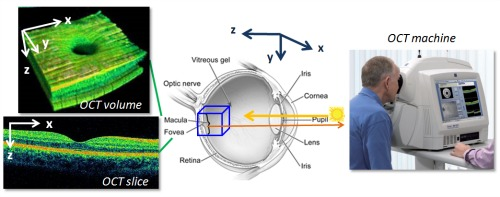
\includegraphics[width=0.7\linewidth]{AAUgraphics/pt1/oct_machine}
	\end{center}
	
\end{frame}

%%%%%%%%%%%%%%%%%%%%%%%%%%
%\subsection{Investigación en OCT y participación de América Latina}
\begin{frame}{OCT respecto a otras técnicas de imagen médica}
	OCT posee una menor resolución axial a la resonancia magnética (MRI), ubicándose entre el ultrasonido (USI) y la microscopía confocal (CM), llenando el vacío en resolución entre estas técnicas\blfootnote{\tiny{S. Schlachter \emph{et al.} Optical coherence tomography / gastroenterology: advanced OCT, next-gen OCT for esophagus. \emph{Bio Optics}, 2013.}}.
	
	\vfill
	%\blfootnote{\tiny{S. Schlachter \emph{et al.} Optical coherence tomography / gastroenterology: advanced oct: next-gen OCT for esophagus. \emph{Bio Optics}, 2013.}}
	%\begin{center}
	%\begin{multicols}{2}
	%	\vspace*{0.5cm}
	%	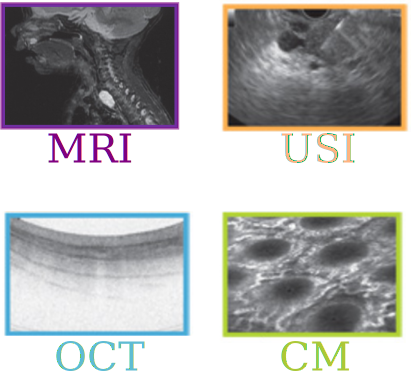
\includegraphics[width=0.9\linewidth]{AAUgraphics/pt1/resolucion}
	%	\newpage
	%	\vspace*{0.5cm}
	%	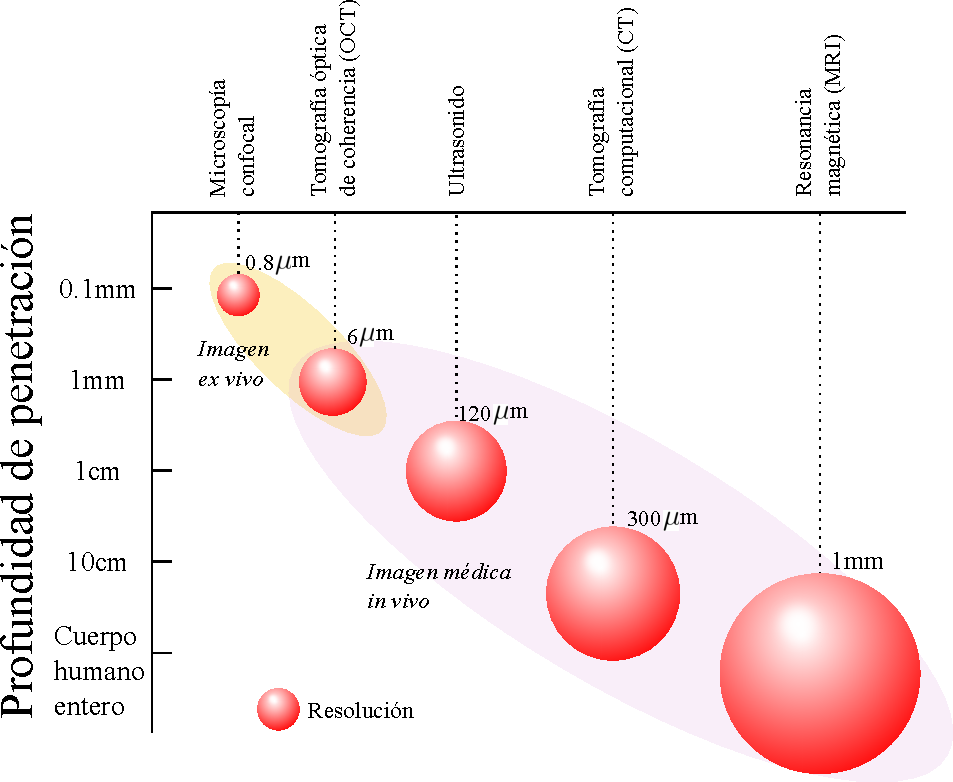
\includegraphics[width=1\linewidth]{AAUgraphics/pt1/Carlos_oct_resolucion}
	%\end{multicols}
	%\end{center}
	\vspace*{0.5cm}
	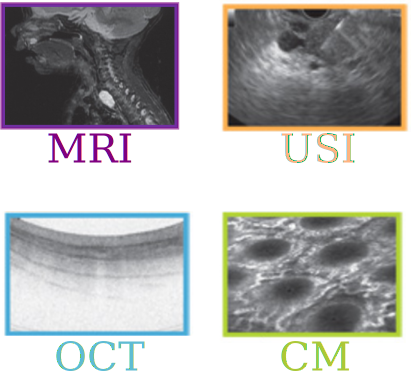
\includegraphics[width=0.4\linewidth]{AAUgraphics/pt1/resolucion}%
	%\vspace*{0.5cm}
	\hspace*{0.5cm}
	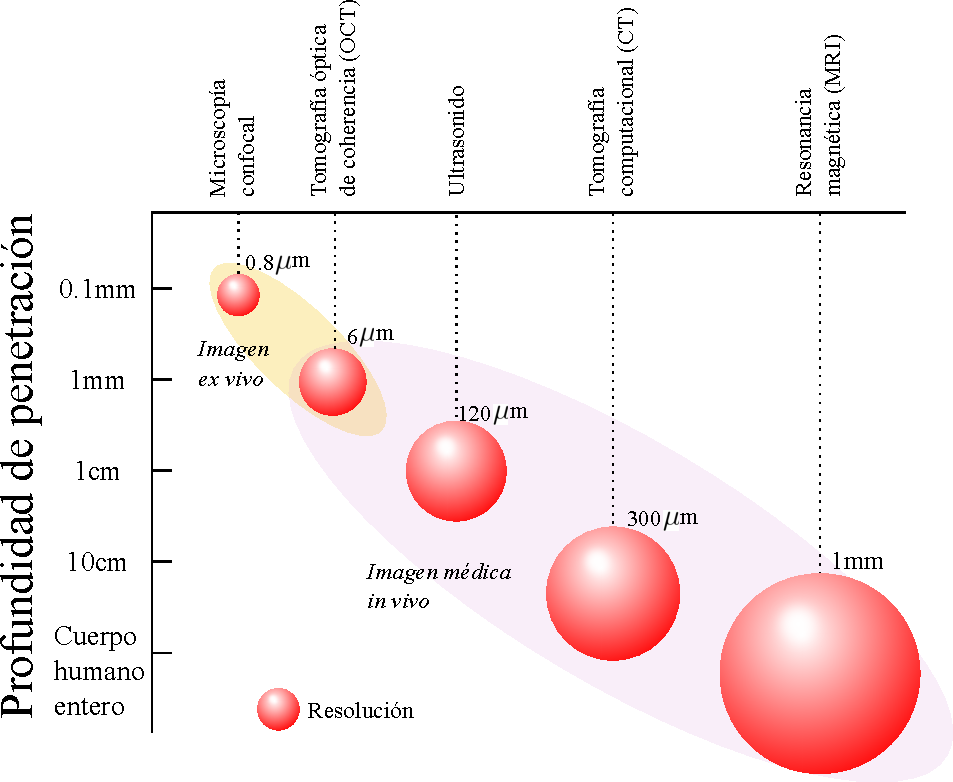
\includegraphics[width=0.55\linewidth]{AAUgraphics/pt1/Carlos_oct_resolucion}
\end{frame}

%%%%%%%%%%%%%%%%%%%%%%%%%%
%\subsection{Investigación en OCT y participación de América Latina}
\begin{frame}{Investigación y participación de Latinoamérica en OCT}{Publicaciones por año}
	%Publicaciones por año\blfootnote{\tiny{J. Fujimoto \emph{et al.} The development, commercialization and impact of optical coherence tomography. \emph{Invest Ophthalmol Vis Sci,} \textbf{57}: OCT1-OCT13, 2016.}}.
	\blfootnote{\tiny{J. Fujimoto \emph{et al.} The development, commercialization and impact of optical coherence tomography. \emph{Invest Ophthalmol Vis Sci,} \textbf{57}: OCT1-OCT13, 2016.}}
	%\vspace*{0.5cm}
	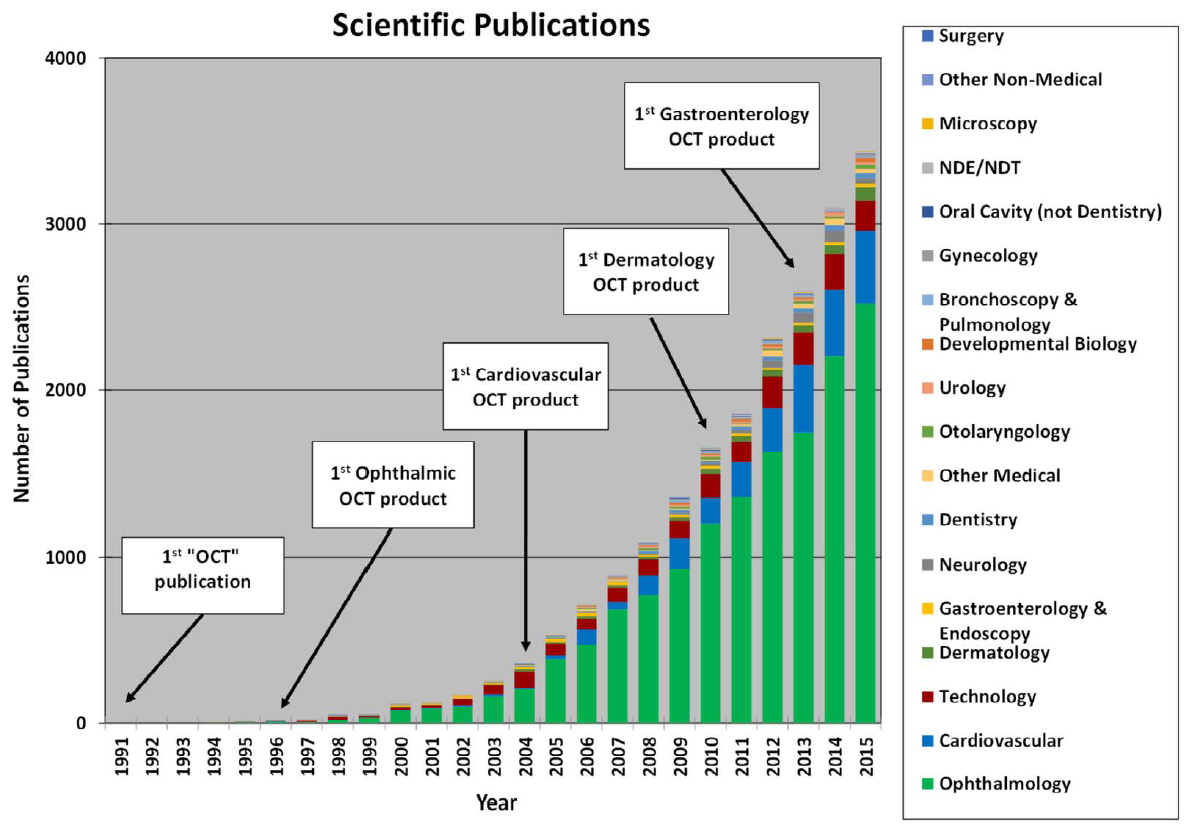
\includegraphics[width=0.95\linewidth]{AAUgraphics/pt1/oct_pub_by_year}%
	%\vspace*{0.5cm}
	%\hspace*{0.5cm}
	%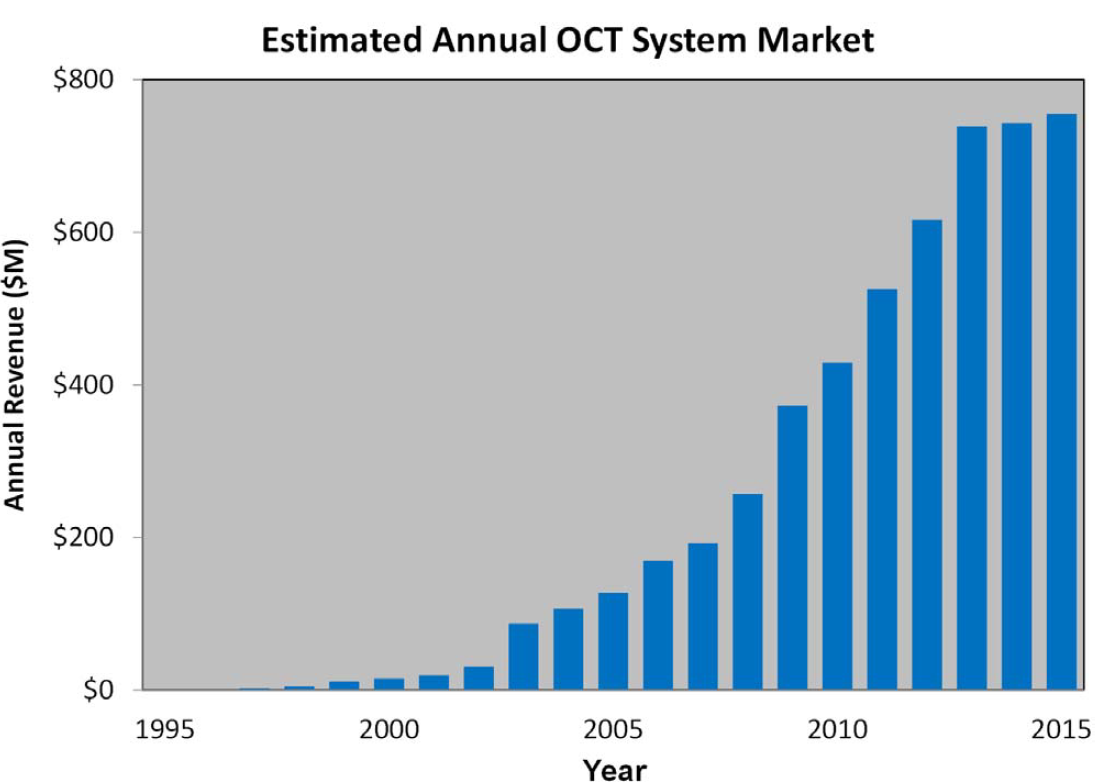
\includegraphics[width=0.4\linewidth]{AAUgraphics/pt1/oct_market}
\end{frame}

%\addtocounter{framenumber}{-1}
\begin{frame}{Investigación y participación de Latinoamérica en OCT}{Mapa de los grupos de investigación}
	%Mapa de los grupos de investigación\blfootnote{\tiny{J. Fujimoto \emph{et al.} The development, commercialization and impact of optical coherence tomography. \emph{Invest Ophthalmol Vis Sci,} \textbf{57}: OCT1-OCT13, 2016.}}.
	\blfootnote{\tiny{J. Fujimoto \emph{et al.} The development, commercialization and impact of optical coherence tomography. \emph{Invest Ophthalmol Vis Sci,} \textbf{57}: OCT1-OCT13, 2016.}}
	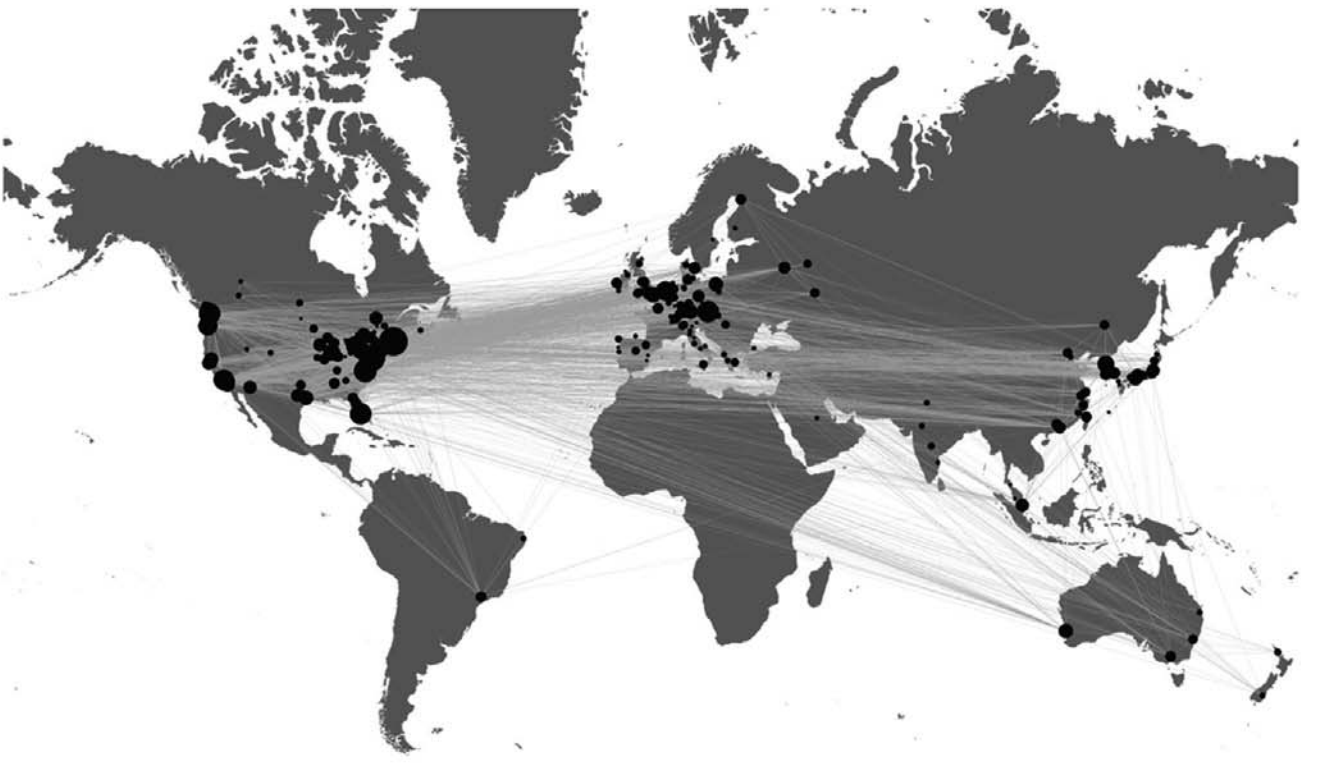
\includegraphics[width=1\linewidth]{AAUgraphics/pt1/oct_groups_2015}
\end{frame}

\addtocounter{framenumber}{-1}
\begin{frame}{Investigación y participación de Latinoamérica en OCT}{Mapa de los grupos de investigación}
	%Mapa de los grupos de investigación\blfootnote{\tiny{J. Fujimoto \emph{et al.} The development, commercialization and impact of optical coherence tomography. \emph{Invest Ophthalmol Vis Sci,} \textbf{57}: OCT1-OCT13, 2016.}}.
	\blfootnote{\tiny{J. Fujimoto \emph{et al.} The development, commercialization and impact of optical coherence tomography. \emph{Invest Ophthalmol Vis Sci,} \textbf{57}: OCT1-OCT13, 2016.}}
	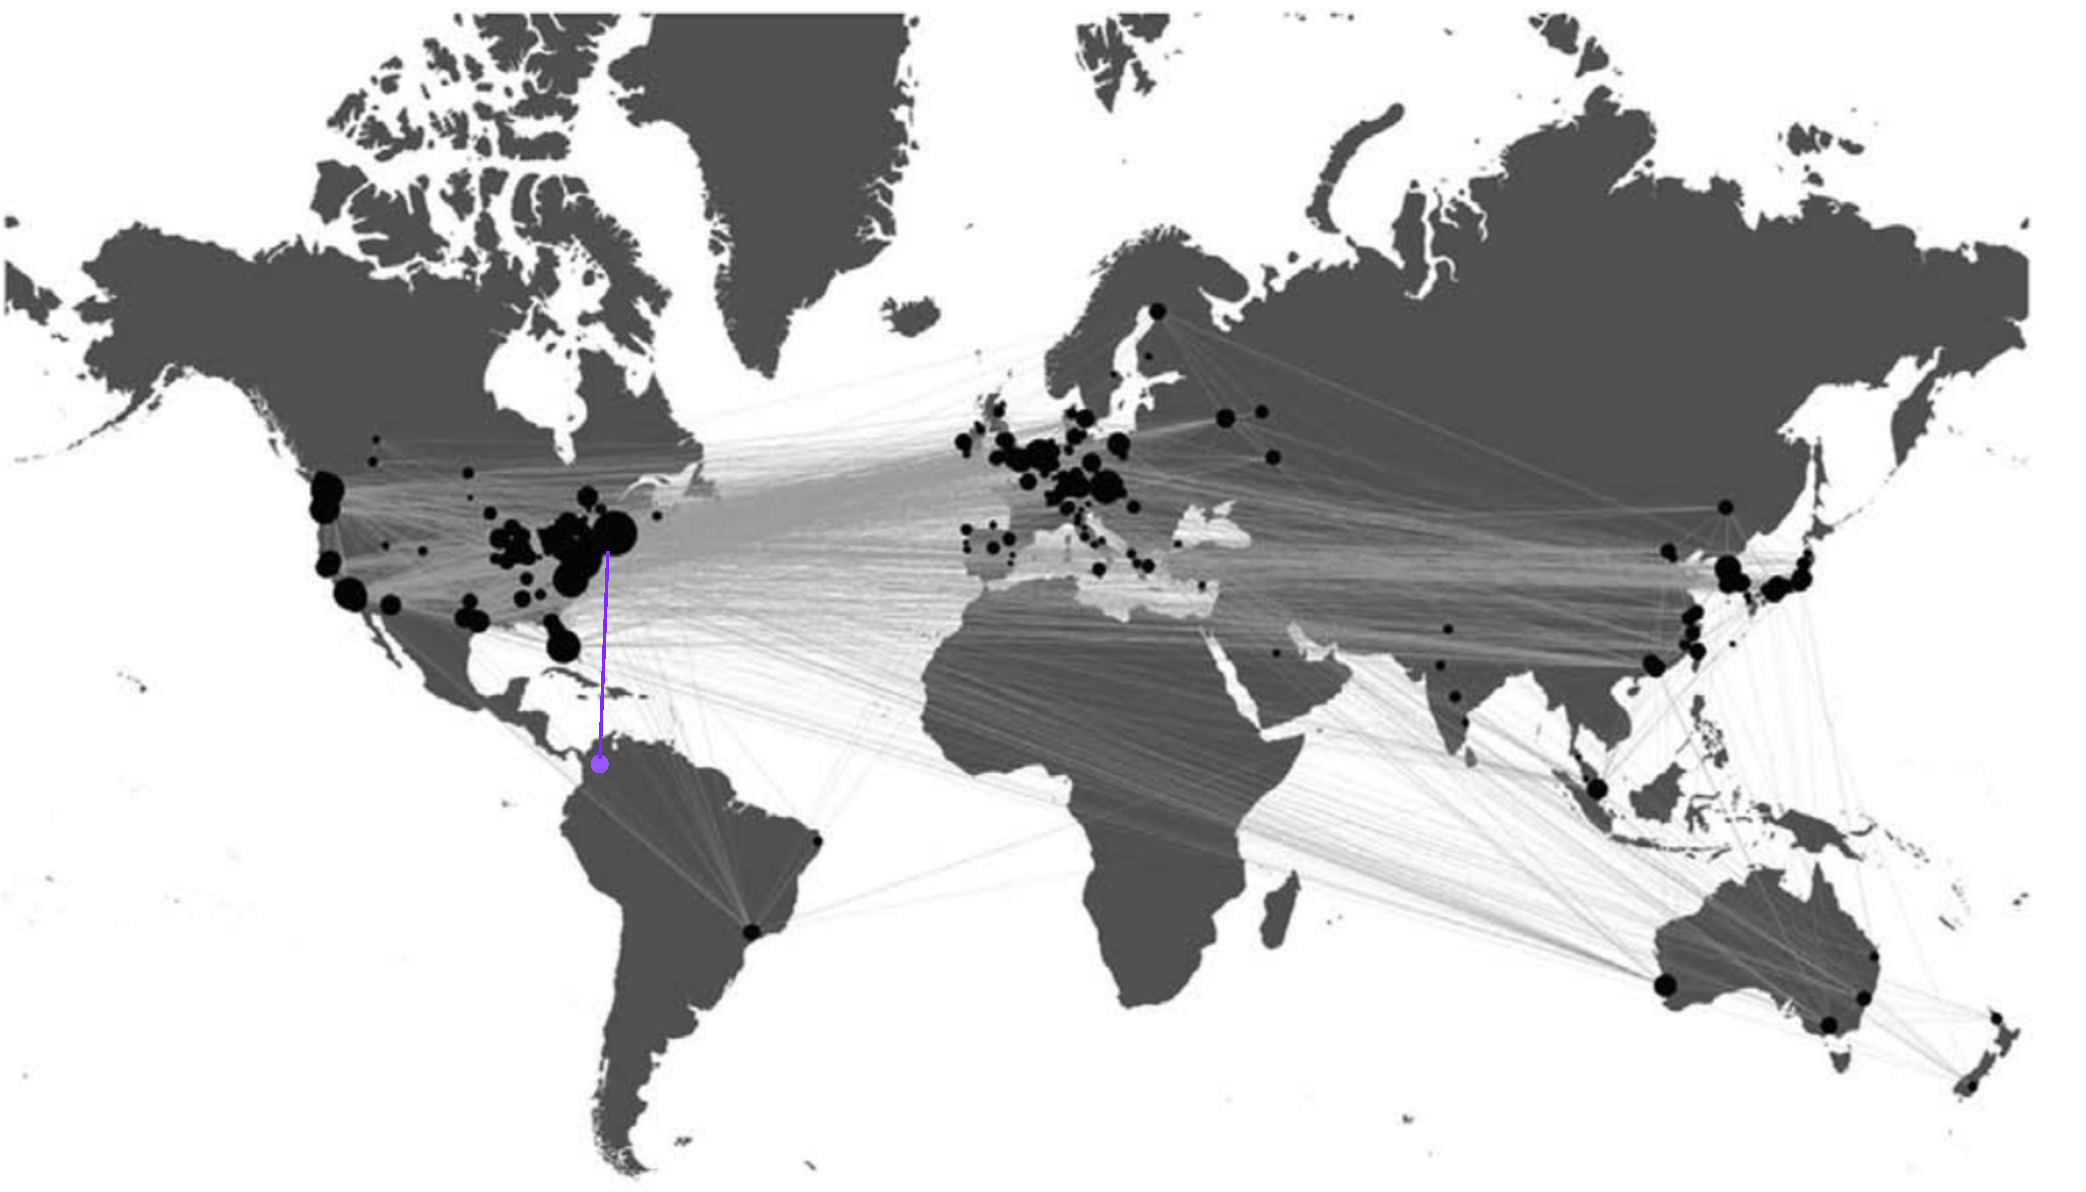
\includegraphics[width=1\linewidth]{AAUgraphics/pt1/Maps_2}
\end{frame}

%%%%%%%%%%%%%%%%%%%%%%%%%%
%\subsection{Aplicaciones de OCT}
%\begin{frame}{Aplicaciones de OCT}{Oftalmología}
%	%Detección y seguimiento de enfermedades\blfootnote{{\tiny A. Girach \emph{et al.} Optical coherence tomography. \emph{Springer,} 2016.}}.
%	\blfootnote{{\tiny A. Girach \emph{et al.} Optical coherence tomography. \emph{Springer,} 2016.}}
%	\begin{center}
%		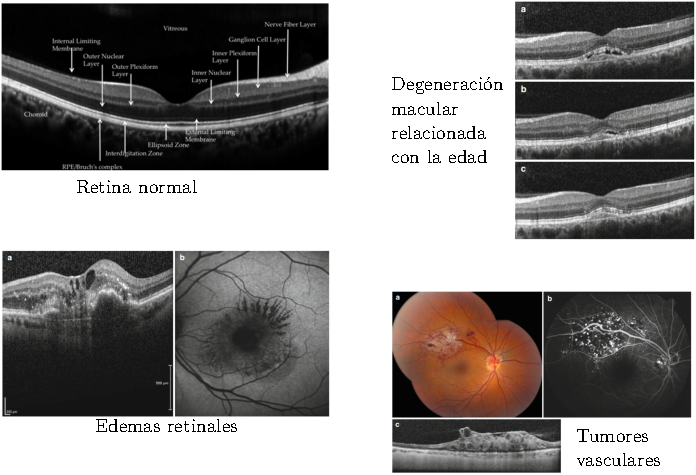
\includegraphics[width=1\linewidth]{AAUgraphics/pt1/oct_retinal}
%	\end{center}
%	
%\end{frame}

%%%%%%%%%%%%%%%%%%%%%%%%%%
%\subsection{Aplicaciones de OCT}
\begin{frame}{Aplicaciones de OCT}{Intravascular}
	%Arterias y venas\blfootnote{\tiny{X. Bai \emph{et al.} Intravascular optical-resolution photoacustic tomography with 1.1 mm diameter catheter. \emph{PLOS ONE,} \textbf{9}(3): e92463, 2014.}}\blfootnote{\tiny{W. Drexler \emph{et al.} Optical coherence tomography: Technology and applications. \emph{Springer,} 2015.}}.
	\blfootnote{\tiny{X. Bai \emph{et al.} Intravascular optical-resolution photoacustic tomography with 1.1 mm diameter catheter. \emph{PLOS ONE,} \textbf{9}(3): e92463, 2014.}}\blfootnote{\tiny{W. Drexler \emph{et al.} Optical coherence tomography: Technology and applications. \emph{Springer,} 2015.}}
		
	\begin{center}
		\includegraphics[width=1\linewidth]{AAUgraphics/pt1/oct_iv}
	\end{center}
	
\end{frame}

%%%%%%%%%%%%%%%%%%%%%%%%%%
%\subsection{Aplicaciones de OCT}
%\begin{frame}{Aplicaciones de OCT}{Gastroenterología}
%	%En gastroenterología para el esófago\blfootnote{\tiny{W. Drexler \emph{et al.} Optical coherence tomography: Technology and applications. \emph{Springer,} 2015.}}.
%	\blfootnote{\tiny{W. Drexler \emph{et al.} Optical coherence tomography: Technology and applications. \emph{Springer,} 2015.}}
%		
%	\begin{center}
%		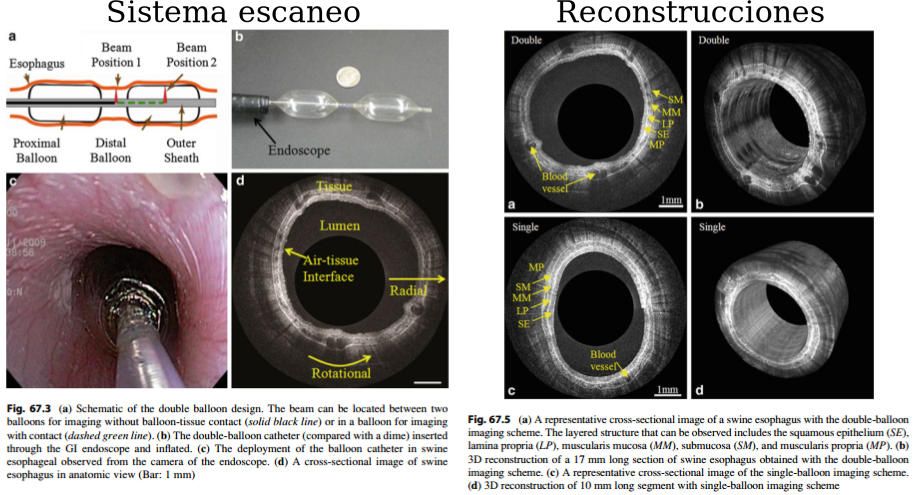
\includegraphics[width=1\linewidth]{AAUgraphics/pt1/oct_gi}
%	\end{center}
%	
%\end{frame}

%%%%%%%%%%%%%%%%%%%%%%%%%%
%\subsection{Aplicaciones de OCT}
%\begin{frame}{Aplicaciones de OCT}{Odontología}
%	Este es otro fram dummy
%\end{frame}

%%%%%%%%%%%%%%%%%%%%%%%%%%
\subsection{Planteamiento del problema}
\begin{frame}{Planteamiento del problema}
	Como técnica de imagen coherente presenta problemas asociados con la fase, ya sea por el sistema óptico o por las características de la técnica, reflejándose como pérdidas en la calidad de las imágenes.
	
	\vfill
	\begin{multicols}{2}
		\centering
		Sistema de escaneo
		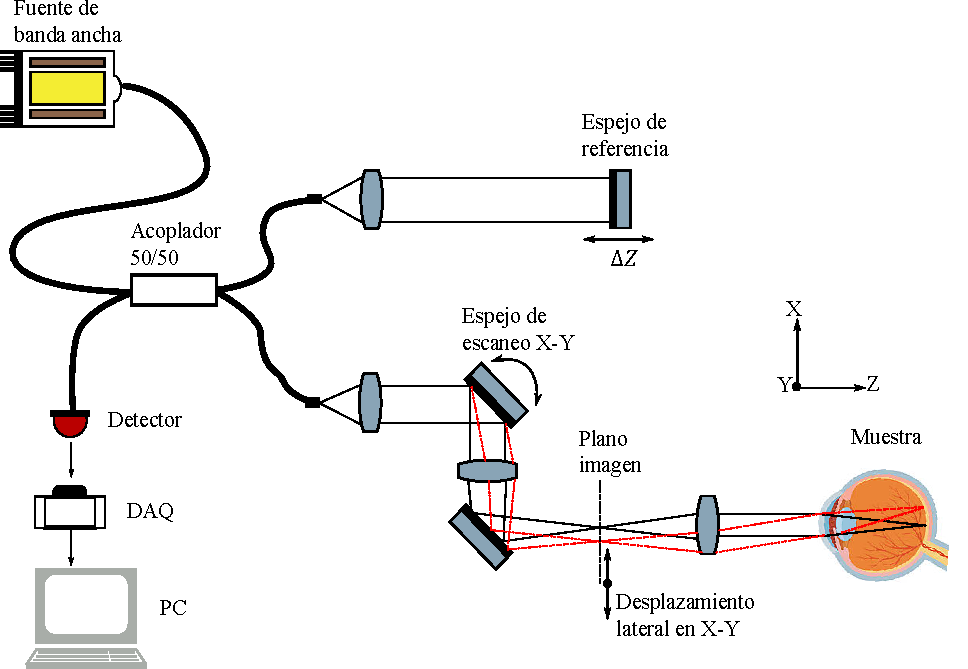
\includegraphics[width=1\linewidth]{AAUgraphics/pt2/scaning_system_oc}
		\newpage
		Imagen con ruido por \emph{speckle}
		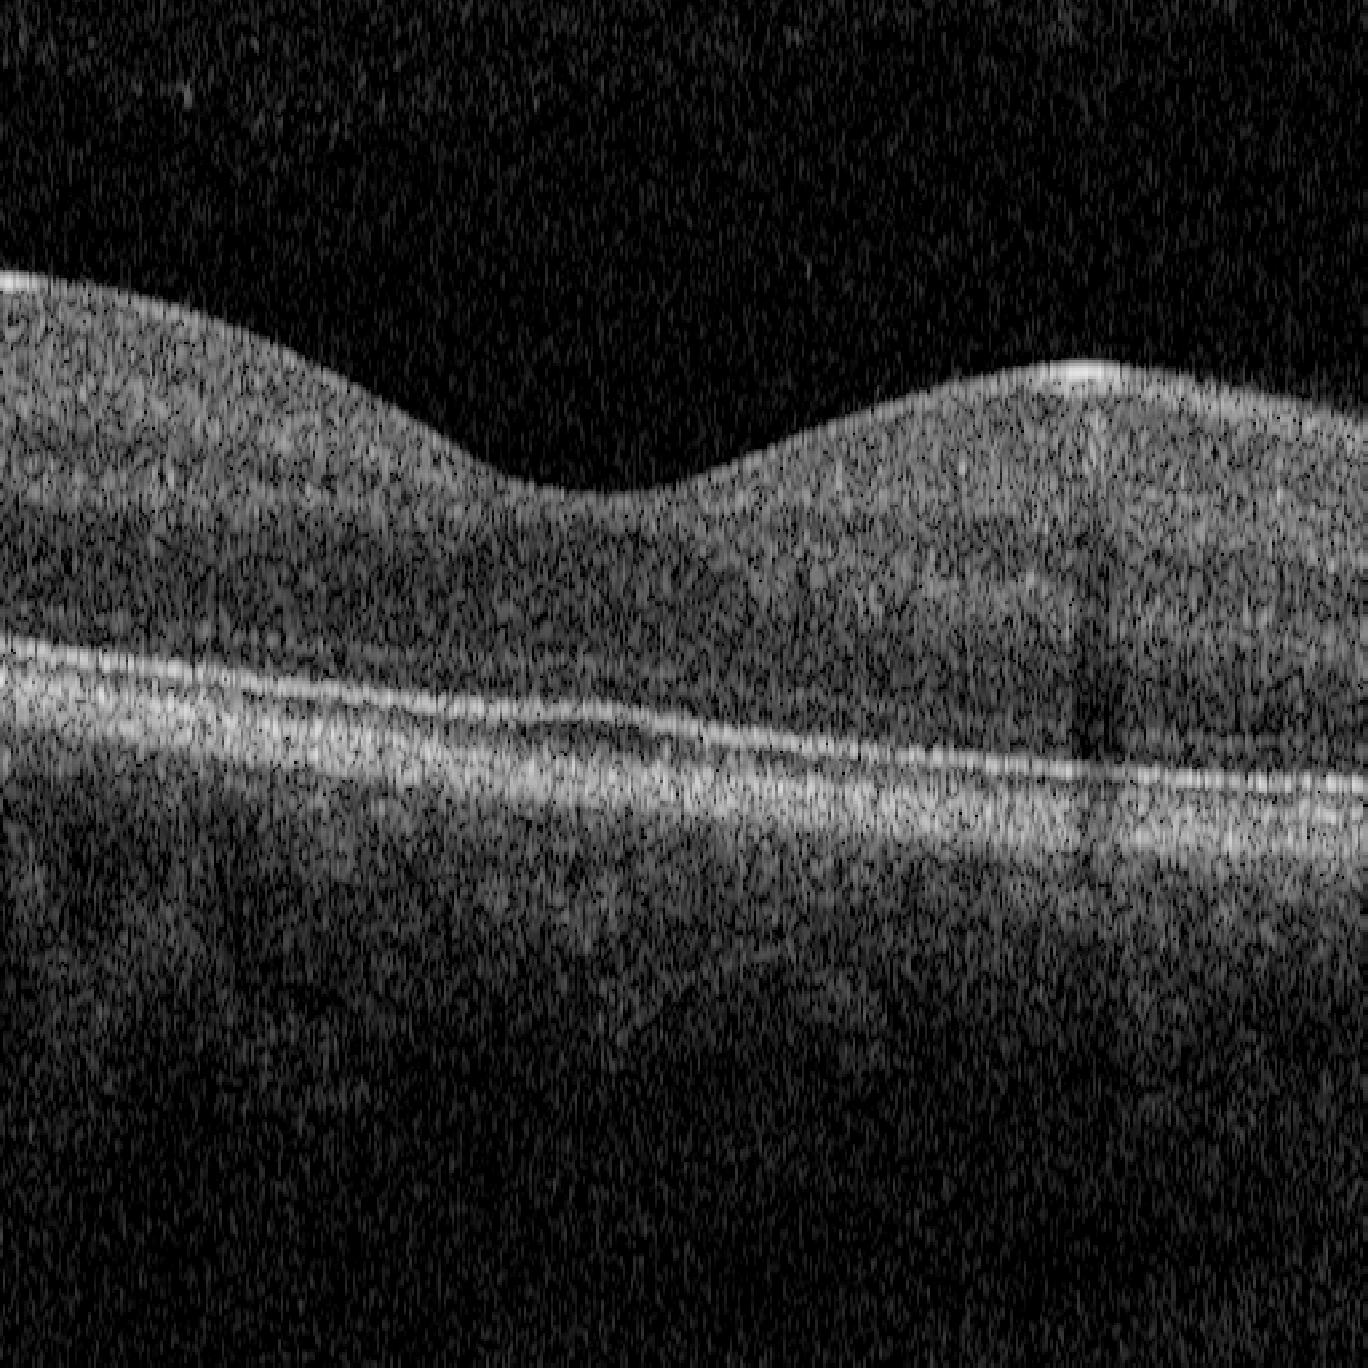
\includegraphics[width=0.8\linewidth]{AAUgraphics/pt3/Retinal_NoisyImage_Bscan128}
	\end{multicols}
\end{frame}


%%%%%%%%%%%%%%%%%%%%%%%%%%
\subsection{Objetivos}
\begin{frame}{Objetivos}
	\begin{block}{Objetivo general}
		{\normalsize Estabilizar la fase en tomografía óptica de coherencia mediante posprocesamiento.}
	\end{block}
\end{frame}

	\addtocounter{framenumber}{-1}
\begin{frame}{Objetivos}
	\begin{block}{Objetivo general}
		{\normalsize Estabilizar la fase en tomografía óptica de coherencia mediante posprocesamiento.}
	\end{block}
	%		\begin{block}{Objetivos específicos}
	%			\begin{itemize}
	%				\item<1-> {\small Identificar el estado de arte de la tomografía óptica de coherencia en aplicaciones biomédicas.}
	%				\item<2-> {\small Implementar un sistema óptica de prueba de concepto de campo completo en la tomografía óptica de coherencia.}
	%				\item<3->{\small  Realizar una simulación del muestreo y la formación de imagen en la tomografía óptica de coherencia, incluyendo elementos de corrupción de fase.}
	%				\item<4-> {\small Desarrollar un método de posprocesamiento que permita recuperar el mapa de corrupción de la imagen simulada anteriormente.}
	%				\item<5-> {\small Comprobar experimentalmente la funcionalidad del algoritmo propuesto con datos experimentales suministrados por el \textit{Wellman Center for Photomedicine, Harvard Medical School and Massachusetts General Hospital.}}
	%			\end{itemize}
	%	
	%		\end{block}
	
	\begin{block}{Objetivos específicos}
		\begin{itemize}
			\item<1-> {\color{blue} Identificar el estado del arte.}
			\item<2-> {\color{green!40!black!60} Implementar un sistema óptico a nivel del laboratorio.}
			\item<3-> {\color{magenta} Realizar simulaciones, incluyendo elementos de corrupción de fase.}
			\item<4-> {\color{cyan} Desarrollar algoritmos de posprocesamiento.}
			\item<5-> {\color{teal} Comprobar experimentalmente los algoritmos.}
		\end{itemize}
		
	\end{block}
\end{frame}



%---------------------------------------------------------------%
\section{Aspectos teóricos y prácticos de OCT}

% Section frame
\begin{frame}{Contenido}
	%\addtocounter{framenumber}{-1}
	\tableofcontents[currentsection]
\end{frame}

%%%%%%%%%%%%%%%%%%%%%%%%%%
\subsection{Marco teórico}
%\subsubsection{Interferometría de baja coherencia}
\begin{frame}{Marco teórico}{Interferometría de baja coherencia: Esquema}
	\begin{multicols}{2}
	\centering
	Esquema interferómetro
	\hspace*{-0.6cm}
	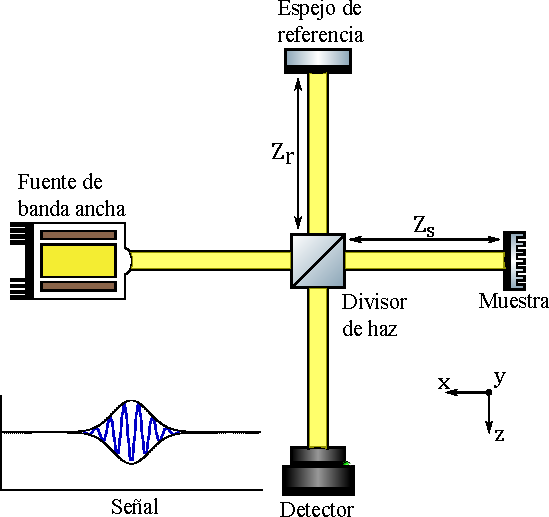
\includegraphics[width=0.9\linewidth]{AAUgraphics/pt2/Carlos_oct_scheme}
	\newpage
	\pause
	Sistema de escaneo
	\hspace*{-0.8cm}
	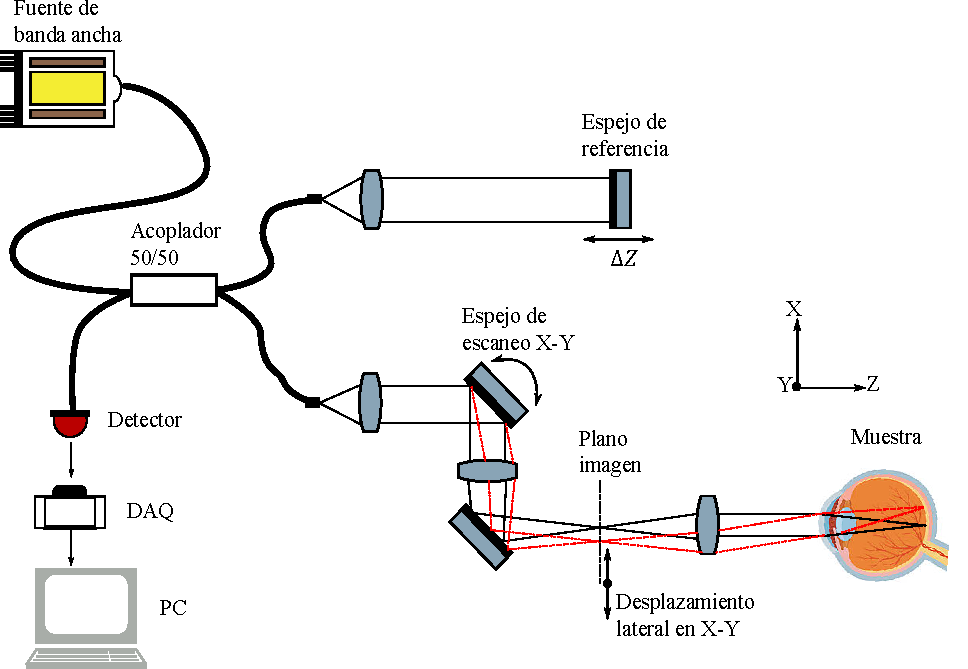
\includegraphics[width=1.2\linewidth]{AAUgraphics/pt2/scaning_system_oc}
	\end{multicols}
		
	\vfill
	
%	Interferencia entre los campos referencia $E_R$ y objeto $E_s$
		\begin{equation*}
			I(k,\omega) = \frac{1}{2} \lvert E_R+E_S \rvert^2  = \frac{1}{2} (E_R+E_S)(E_R+E_S)^\ast	
		\end{equation*}
\end{frame}

\begin{frame}{Marco teórico}{Interferometría de baja coherencia: Teoría}
	\begin{tikzpicture}[remember picture,overlay]
		\node[xshift=-4.3cm,yshift=-3.5cm] at (current page.north east) {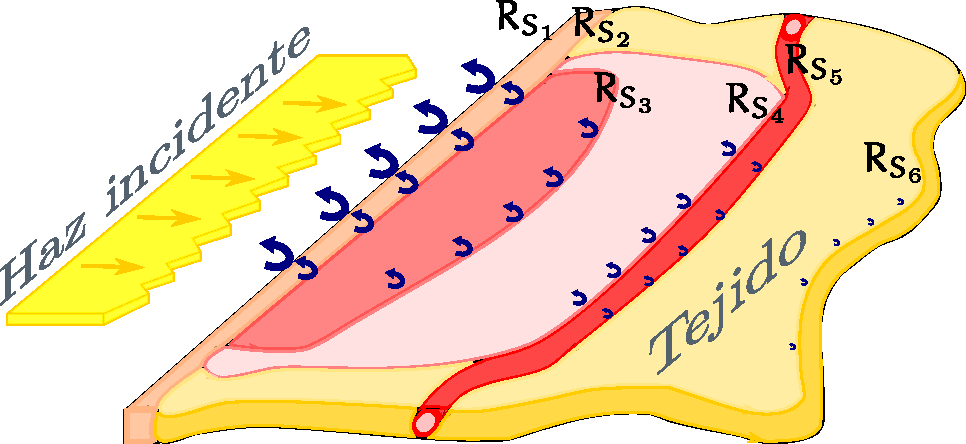
\includegraphics[width=4.0cm]{AAUgraphics/pt2/Tissue_backscattering}};
		\node[xshift=-4.3cm,yshift=-4.8cm] at (current page.north east) {Interacción luz-tejido};
		
	\end{tikzpicture}
	
%	\begin{tikzpicture}[remember picture,overlay]
%	\node[xshift=-4cm,yshift=-4.3cm] at (current page.north east) {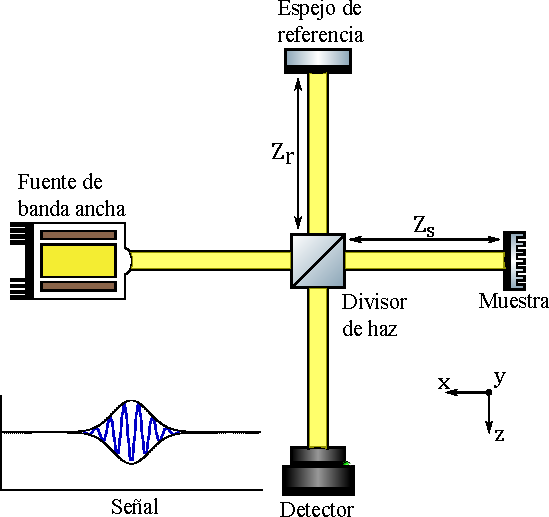
\includegraphics[width=3cm]{AAUgraphics/pt2/Carlos_oct_scheme}};
%	\end{tikzpicture}
	\vspace*{-0.5cm}
	{\scriptsize 		
		\begin{equation*}
			r_S(z_S) = \sum_{n=1}^{N} r_{S_n} \delta[(z_S - z_{S_n})] \quad {\color{blueEQ}R_{S_n}} = \lvert r_{S_n} \rvert^2
		\end{equation*}
		\pause
		\begin{equation*}
			E_i(k,\omega) = s(k,\omega) e^{i(kz - \omega t)}
		\end{equation*}
		%\pause
		\begin{equation*}
			E_R = \frac{E_i}{\sqrt{2}}r_Re^{i2kz_R} \quad E_S = \frac{E_i}{\sqrt{2}} \sum_{n=1}^{N}r_{S_n} e^{i2kz_{S_n}}
		\end{equation*}
		\pause
		\begin{align*}
			I_D(k) = & \overwrite[white!40!violet]{\frac{\rho}{4}\left[ S(k) (R_R + R_{S1} + R_{S2} + ...+R_{Sn}) \right]}{Componente DC}                                                     \\
			         & \overwrite[teal]{+ \frac{\rho}{2} \left[ S(k) \sum_{n=1}^{N} \sqrt{R_R {\color{blueEQ}R_{S_n}}} \left( \cos[2k(z_R - z_{S_n})] \right) \right]}{Términos de correlación cruzada}         \\
			         & \overwrite[white!40!red]{+ \frac{\rho}{4} \left[ S(k) \sum_{m\neq n=1}^{N} \sqrt{R_{S_n}R_{S_m}} \left( \cos[2k(z_{S_n} - z_{S_m})] \right) \right]}{Términos de autocorrelación} 
		\end{align*}
		%\pause
		\begin{equation*}
			\gamma (z) = e^{-z^2\Delta k^2} \leftrightarrow \mathscr{F}\{\gamma (z)\} = S(k) = \frac{1}{\Delta k \sqrt{\pi}} e^{-\left[\frac{(k-k_0)}{\Delta k}\right]^2}.
		\end{equation*}
	}
		
	%	{\footnotesize 	\begin{align*}
	%		&r_S(z_S) = \sum_{n=1}^{N} r_{S_n} \delta[(z_S - z_{S_n})] \quad R_{S_n} = \lvert r_{S_n} \rvert^2\\
	%		\pause
	%		&E_i(k,\omega) = s(k,\omega) e^{i(kz - \omega t)}\\
	%		&E_R = \frac{E_i}{\sqrt{2}}r_Re^{i2kz_R} \quad E_S = \frac{E_i}{\sqrt{2}} \sum_{n=1}^{N}r_{S_n} e^{i2kz_{S_n}}\\
	%		& I_D(k) = \frac{\rho}{4}\left[ S(k) (R_R + R_{S1} + R_{S2} + ...+R_{Sn}) \right] \notag \\
	%		& + \frac{\rho}{2} \left[ S(k) \sum_{n=1}^{N} \sqrt{R_R R_{S_n}} \left( \cos[2k(z_R - z_{S_n})] \right) \right] \\
	%		& + \frac{\rho}{4} \left[ S(k) \sum_{m\neq n=1}^{N} \sqrt{R_{S_n}R_{S_m}} \left( \cos[2k(z_{S_n} - z_{S_m})] \right) \right]\\
	%		&\gamma (z) = e^{-z^2\Delta k^2} \leftrightarrow \mathscr{F}\{\gamma (z)\} = S(k) = \frac{1}{\Delta k \sqrt{\pi}} e^{-\left[\frac{(k-k_0)}{\Delta k}\right]^2}.
	%		\end{align*}}
		
	%	\begin{align}
	%	r_S(z_S) = \sum_{n=1}^{N} r_{S_n} \delta[(z_S - z_{S_n})] \quad R_{S_n} = \lvert r_{S_n} \rvert^2\\
	%	E_i(k,\omega) = s(k,\omega) e^{i(kz - \omega t)}\\
	%	E_R = \frac{E_i}{\sqrt{2}}r_Re^{i2kz_R}\\
	%	E_S = \frac{E_i}{\sqrt{2}} \sum_{n=1}^{N}r_{S_n} e^{i2kz_{S_n}}\\
	%	I(k,\omega) = \frac{1}{2}\lvert E_R+E_S \rvert^2 = (E_R + E_S)(E_R + E_S)^{\ast}\\
	%	I_D(k, \omega) = \frac{\rho}{2} \bigg\langle \bigg\lvert \frac{s(k, \omega)}{\sqrt{2}} r_R e^{i(2kz_R-\omega t)} + \frac{s(k, \omega)}{\sqrt{2}} \sum_{n=1}^{N} r_{S_n} e^{i(2kz_{S_n} - \omega t)} \bigg\rvert^2 \bigg\rangle\\
	%	I_D(k) &= \frac{\rho}{4}\left[ S(k) (R_R + R_{S1} + R_{S2} + ...+R_{Sn}) \right] \notag \\
	%	& + \frac{\rho}{2} \left[ S(k) \sum_{n=1}^{N} \sqrt{R_R R_{S_n}} \left( \cos[2k(z_R - z_{S_n})] \right) \right] \\
	%	& + \frac{\rho}{4} \left[ S(k) \sum_{m\neq n=1}^{N} \sqrt{R_{S_n}R_{S_m}} \left( \cos[2k(z_{S_n} - z_{S_m})] \right) \right]\\
	%	\gamma (z) = e^{-z^2\Delta k^2} \leftrightarrow \mathscr{F}\{\gamma (z)\} = S(k) = \frac{1}{\Delta k \sqrt{\pi}} e^{-\left[\frac{(k-k_0)}{\Delta k}\right]^2}.
	%	\end{align}
		
\end{frame}

%%%%%%%%%%%%%%%%%%%%%%%%%%%
%%\subsubsection{Interferometría de baja coherencia en el dominio temporal}
\begin{frame}{Marco teórico}{OCT en el dominio temporal (TDOCT)}
	{\small \begin{align*}
		I_D(z_R) = & \frac{\rho}{4}S_0 [R_R+ R_{S1}+ R_{S2}+...]                                                                                  \\ \notag
		           & +\frac{\rho}{2}\left[ S_0 \sum_{n=1}^{N} \sqrt{R_R {\color{blueEQ}R_{S_n}}} e^{-[z_R-z_{S_n}]^2 \Delta k^2}  \cos[2k_0 (z_R-z_{S_n})]\right] 
	\end{align*}}
	
	\begin{center}
		\vfill
		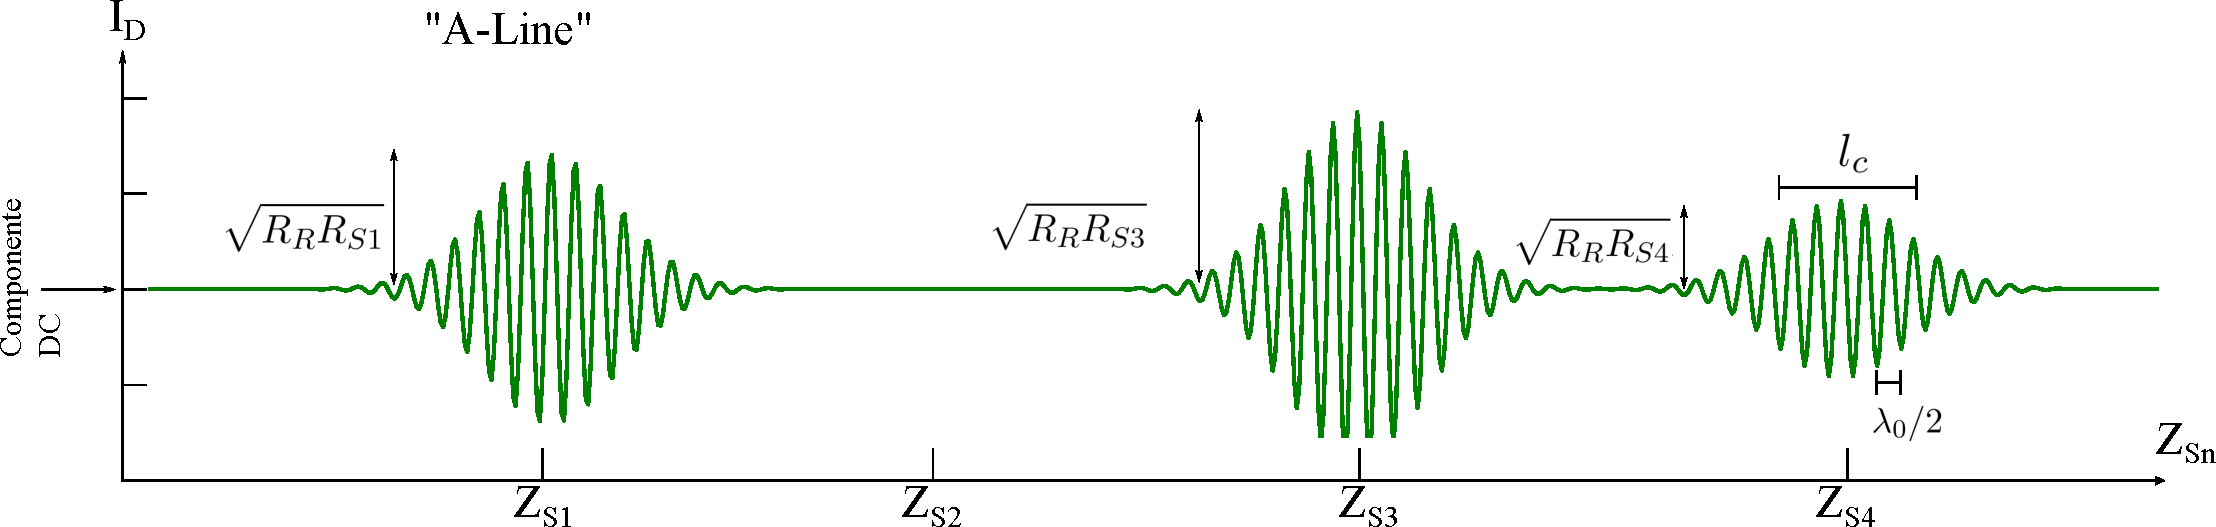
\includegraphics[width=1\linewidth]{AAUgraphics/pt2/A_Line_1Gen}
		\pause
		\vspace*{0.5cm}	
		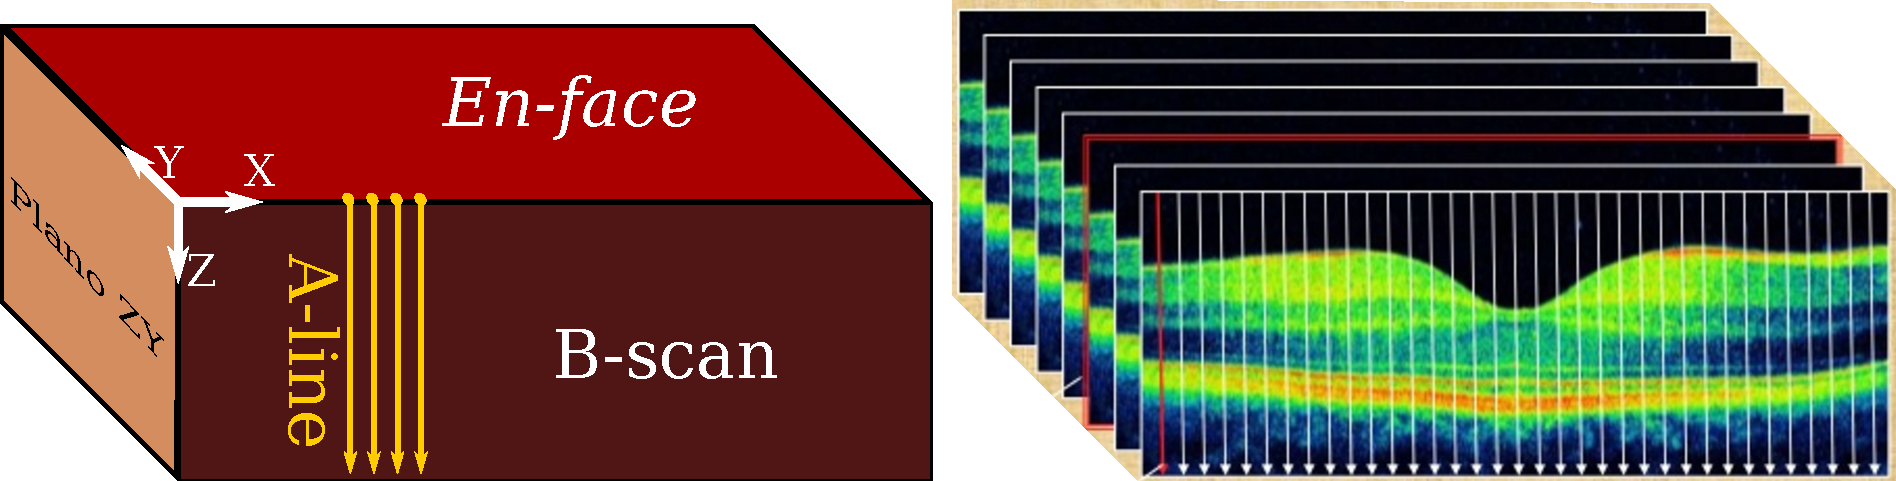
\includegraphics[width=0.7\linewidth]{AAUgraphics/pt2/Imaging_directions}
	\end{center}
	
%	\pause
%	\vfill
%	\begin{equation*}
%		i_D = \rho \langle\lvert E_R\rvert^2 + \lvert E_S \rvert^2 + 2E_R E_S \cos(2 k_0 \overwrite[blue]{\Delta z}{OPD})\rangle
%	\end{equation*}
	
\end{frame}

%%%%%%%%%%%%%%%%%%%%%%%%%%%
%%\subsubsection{Interferometría de baja coherencia en el dominio de Fourier}
%\begin{frame}{Marco teórico}{OCT en el dominio frecuencial (FDOCT)}
%	\begin{equation*}
%		i_D = \rho \langle\lvert E_R\rvert^2 + \lvert E_S \rvert^2 + 2E_R E_S \cos(2 \overwrite[green!20!blue]{k_0}{$\lambda$} \Delta z)\rangle
%	\end{equation*}
%	
%	\pause
%	\vfill
%	{\footnotesize \begin{align*}
%		i_D(z) & = \frac{\rho}{8}\left[\gamma (z) [R_R + R_{S1} + R_{S2} + ...] \right]                                                                       \\ \notag
%		       & + \frac{\rho}{4} \left[\gamma (z) \otimes \sum_{n=1}^{N} \sqrt{R_R {\color{blueEQ}R_{S_n}}}\{\delta[z\pm (2(z_R-z_{S_n}))]\}\right]                          \\
%		       & + \frac{\rho}{8} \left[\gamma (z) \otimes \sum_{m\neq n = 1}^{N} \sqrt{R_{S_n}R_{S_m}} \{\delta [z\pm 2(z_{S_n} - z_{S_m})]\} \right].\notag 
%	\end{align*}}
%	
%	\vfill
%	\begin{center}
%		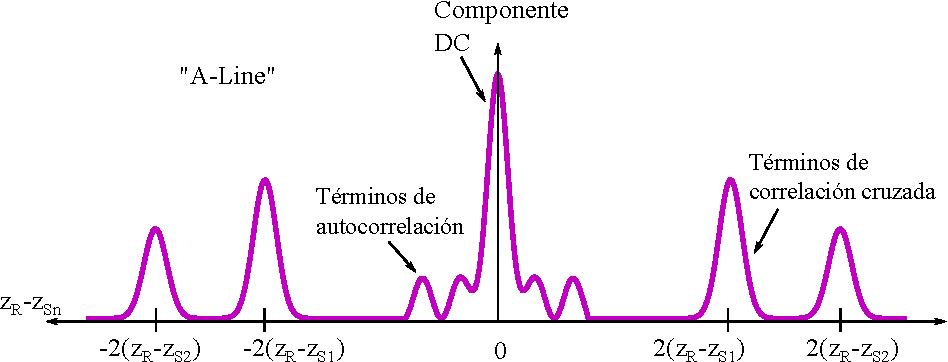
\includegraphics[width=0.7\linewidth]{AAUgraphics/pt2/A_Line_FFT}
%	\end{center}
%	
%	
%\end{frame}

%%%%%%%%%%%%%%%%%%%%%%%%%%
%\subsection[Parámetros importantes]{Parámetros importantes en un sistema de OCT}
%\begin{frame}{Parámetros importantes}{Resolución axial y lateral}
%	Este es un frame dummy
%\end{frame}

%%%%%%%%%%%%%%%%%%%%%%%%%%
\subsection[Sistema de OCT a nivel del laboratorio]{Implementación de un sistema de OCT a nivel del laboratorio}
\begin{frame}{Sistema de OCT a nivel del laboratorio}{Esquema del montaje}
	\begin{multicols}{2}
		\centering
		Esquema
		\includegraphics[width=1.0\linewidth]{AAUgraphics/pt2/Montaje_scheme}
		\newpage
		Montaje experimental
		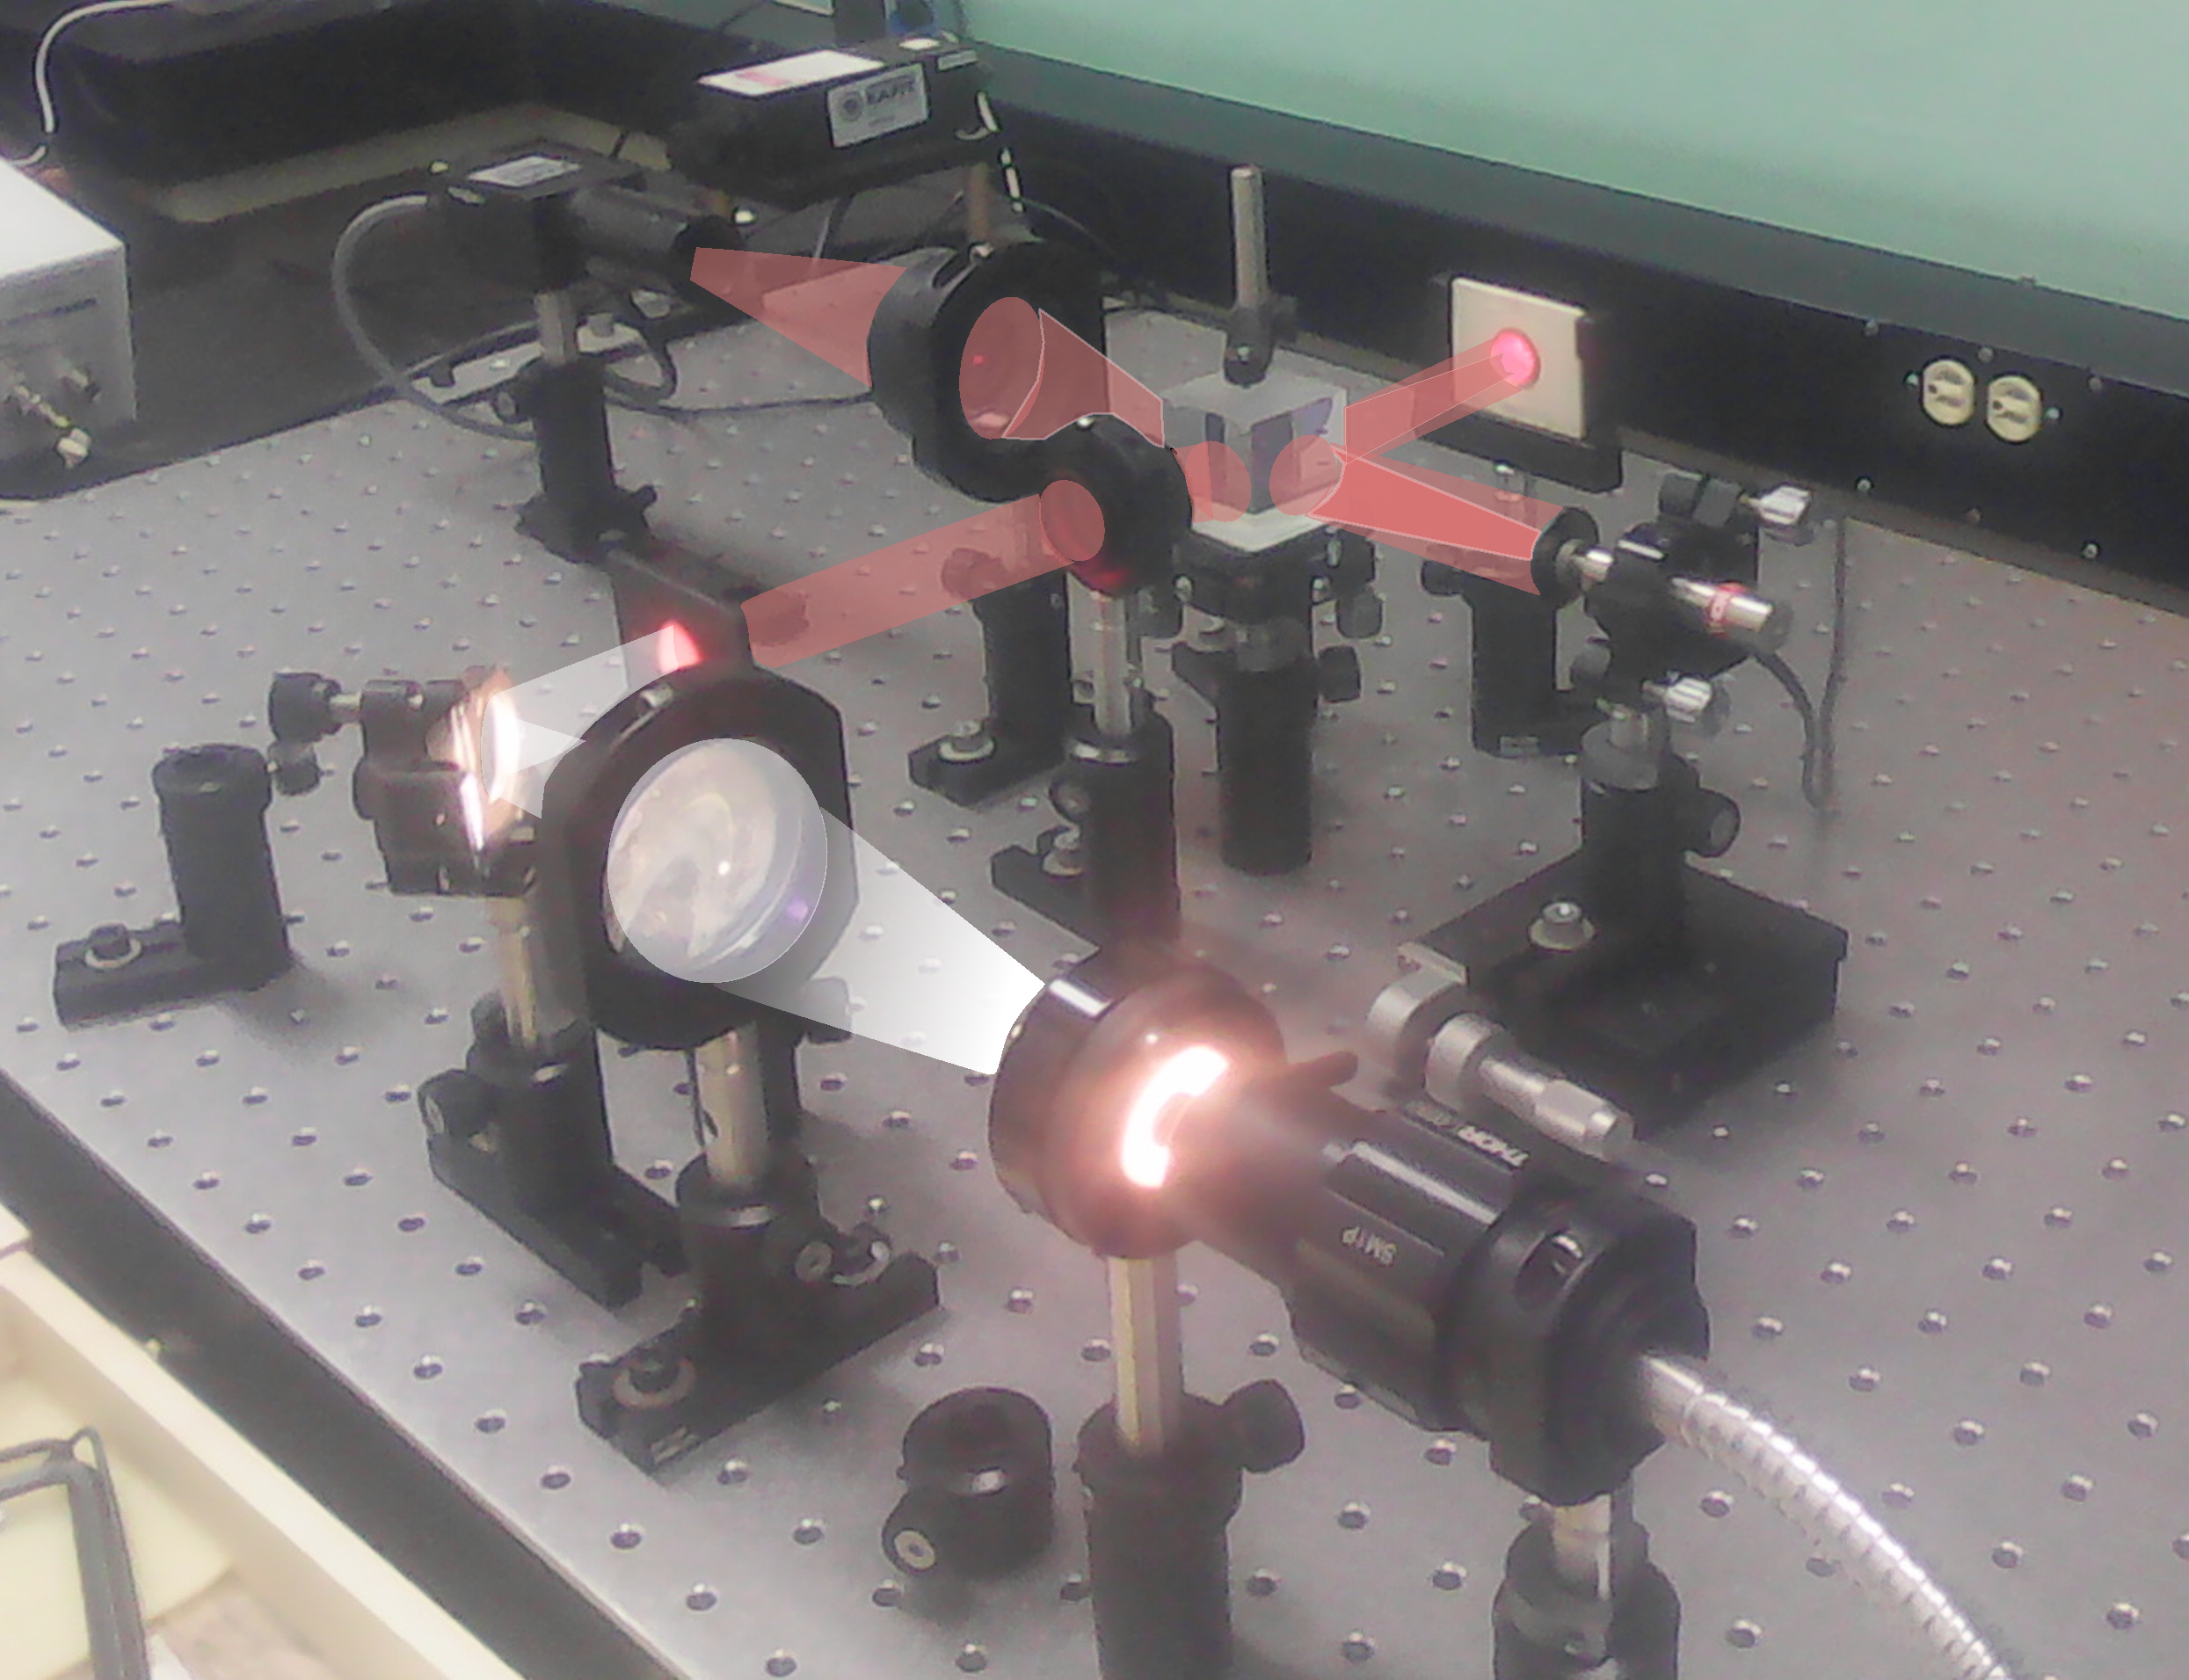
\includegraphics[width=0.8\linewidth]{AAUgraphics/pt2/Montaje}
	\end{multicols}
\end{frame}

%%%%%%%%%%%%%%%%%%%%%%%%%%
%\subsubsection{Características del sistema experimental}
\begin{frame}{Sistema de OCT a nivel del laboratorio}{Características}
	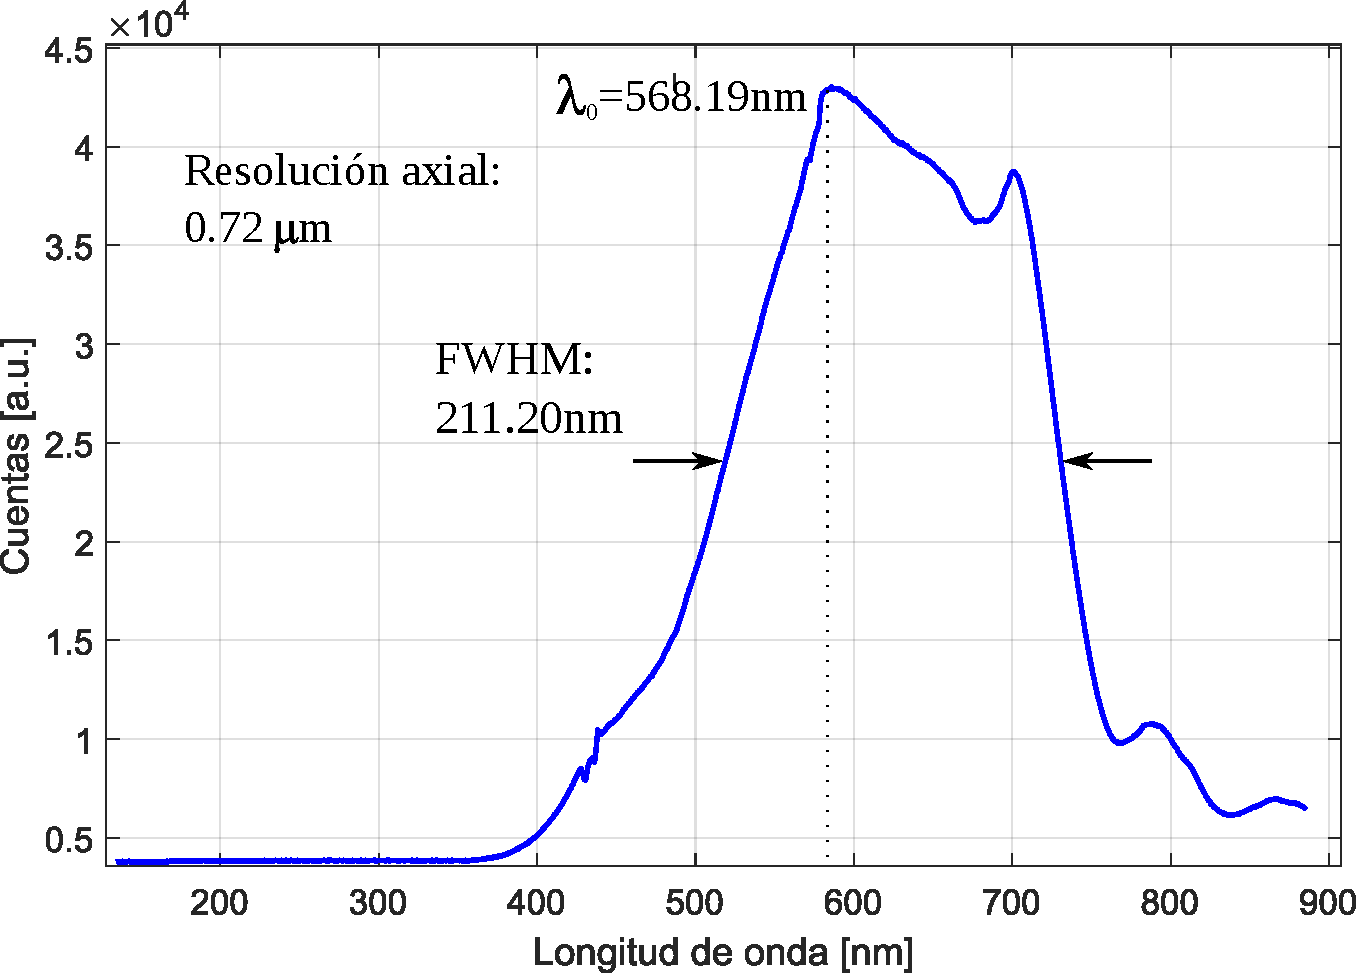
\includegraphics[width=0.42\linewidth]{AAUgraphics/pt2/src_spectrum}
	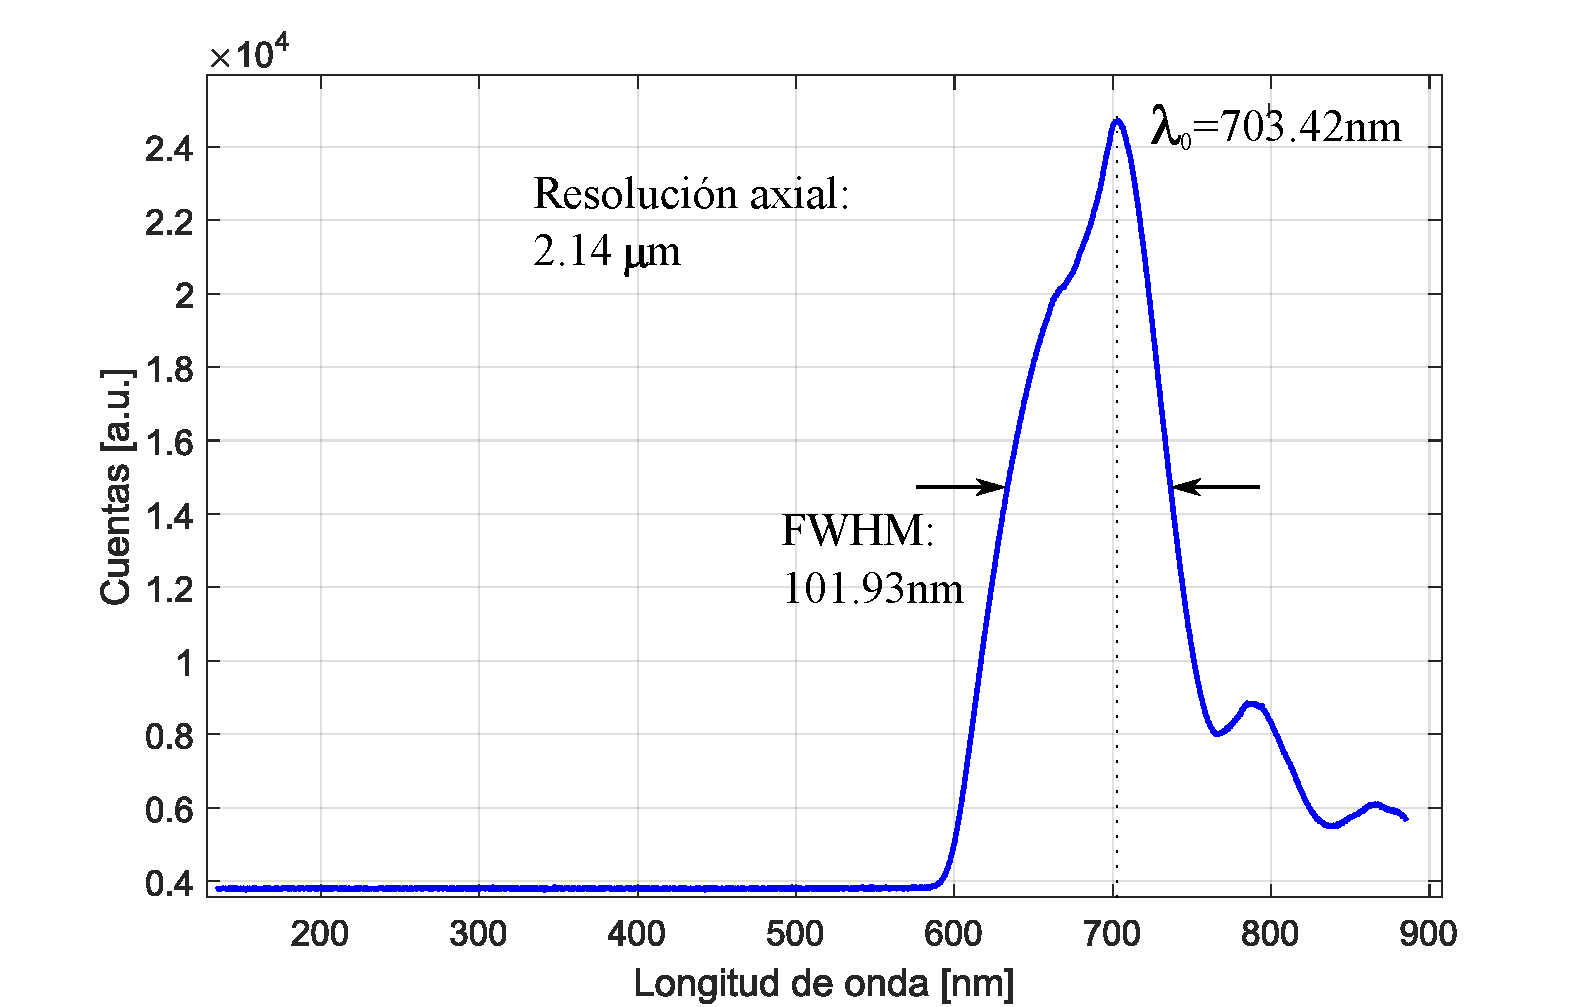
\includegraphics[width=0.49\linewidth]{AAUgraphics/pt2/filt_spectrum}
	\begin{table}
		\begin{tabular}{|c|c|}
			\hline
			\textbf{Parámetro}    &                       \\ 
			\hline
			Resolución lateral    & $3.56\mu m$           \\ 
			\hline
			Resolución axial      & $2.14\mu m$           \\ 
			\hline
			Paso mínimo           & $1\mu m$              \\
			\hline
			Desplazamiento máximo & $1.5cm$               \\ 
			\hline
			Sensibilidad           & $-36dB(10^{-3.6}I_0)$ \\
			\hline
		\end{tabular} 
	\end{table}
\end{frame}

%%%%%%%%%%%%%%%%%%%%%%%%%%
%\subsubsection{Patrones interferencia}
\begin{frame}{Sistema de OCT a nivel del laboratorio}{Patrones de interferencia}
	
	\blfootnote{{\tiny Z.Wang and B. Han. Advanced iterative algorithm for phase extraction of randomly phase-shifted interferograms. \emph{Opt. Lett.}, \textbf{29}(14):1671-1673, 2004.}}
	
	\vspace*{-0.7cm}
	\begin{center}
		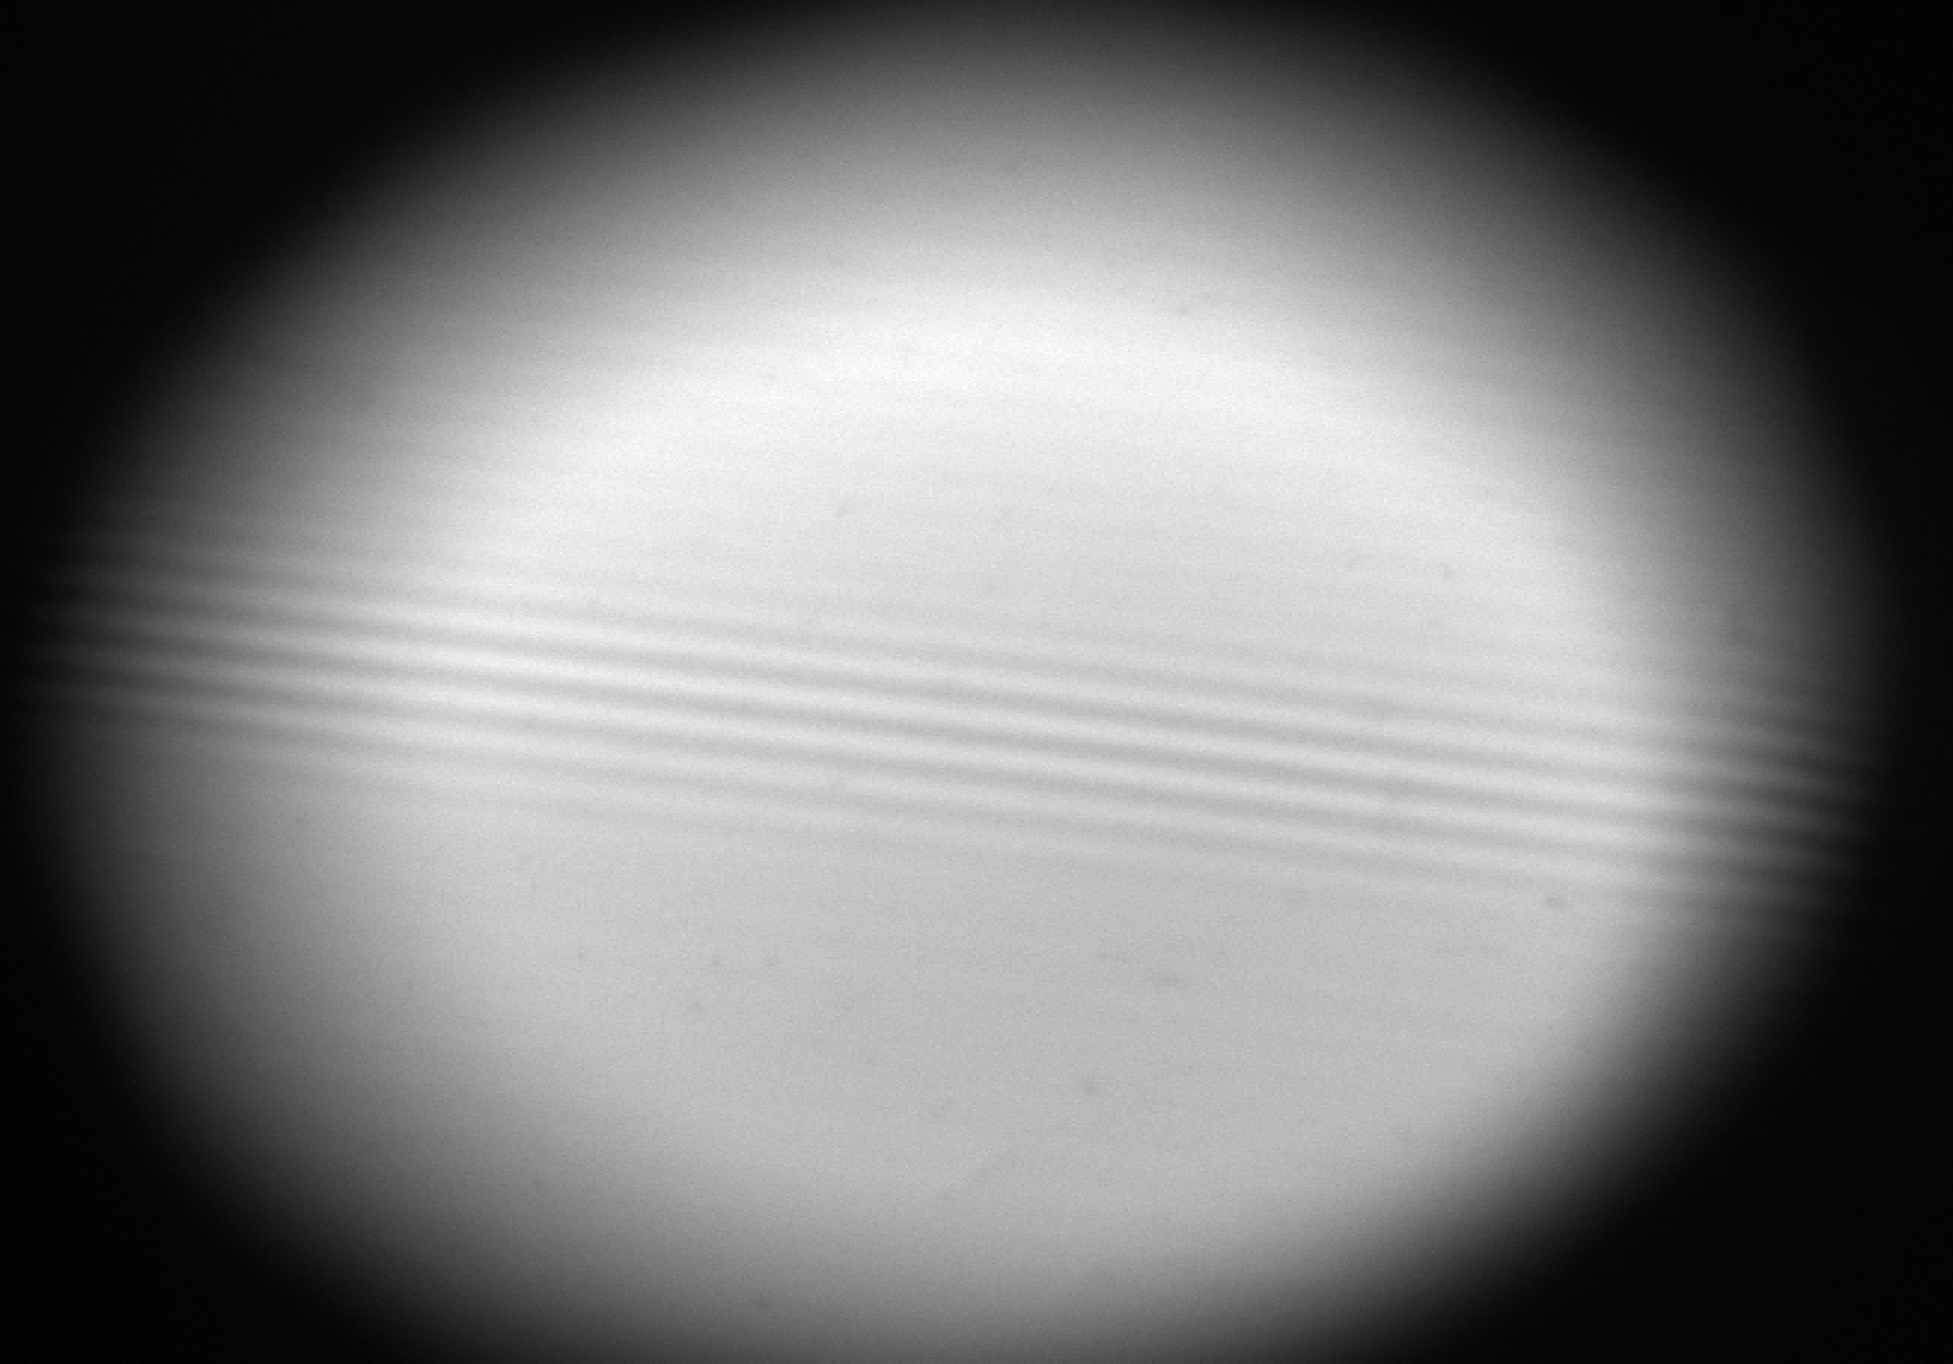
\includegraphics[width=4cm]{AAUgraphics/pt2/PatronInterferencia}
		\hspace*{0.05cm}\pause
		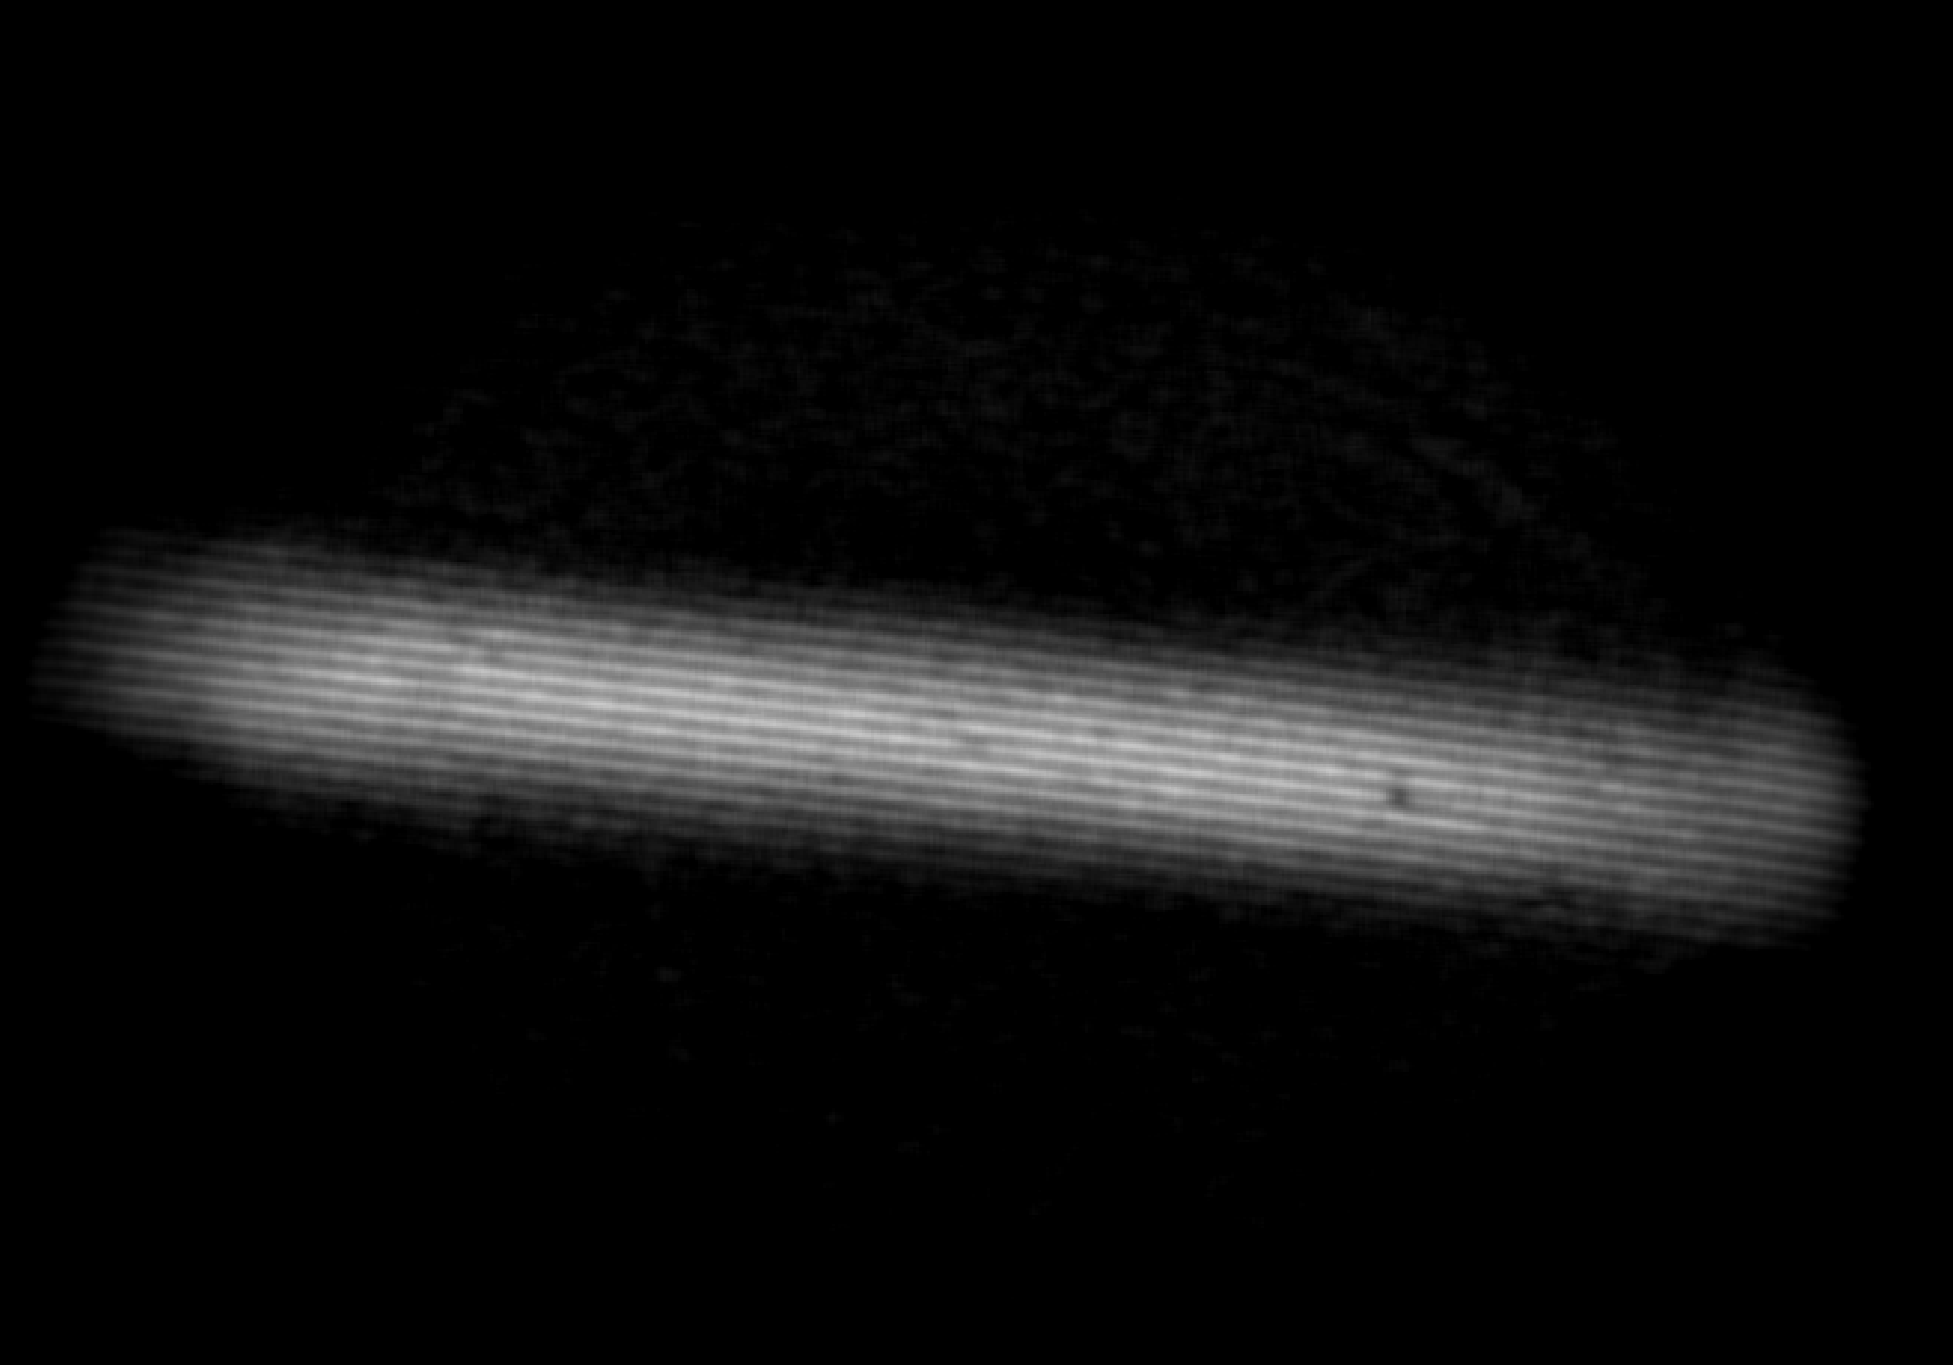
\includegraphics[width=4cm]{AAUgraphics/pt2/Modulacion}\par
		
		\pause
		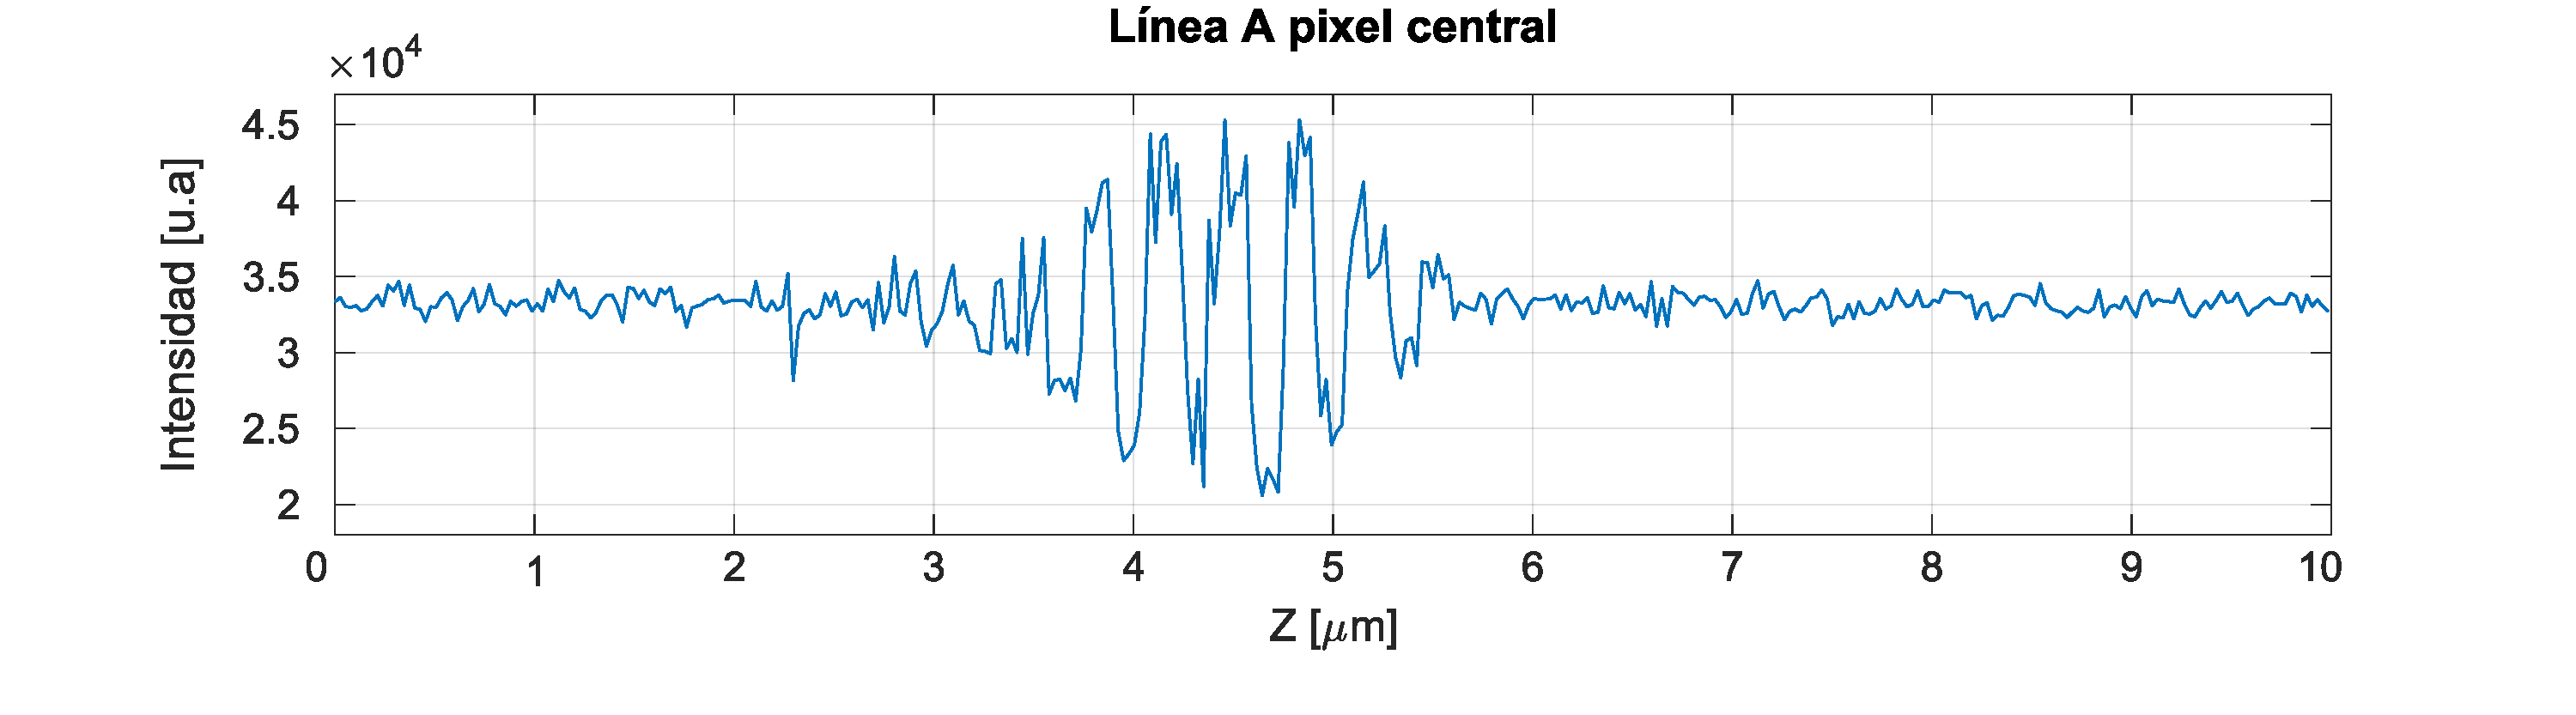
\includegraphics[width=8cm]{AAUgraphics/pt2/LineaAPXCenter} \par
		\vspace*{-0.2cm}
		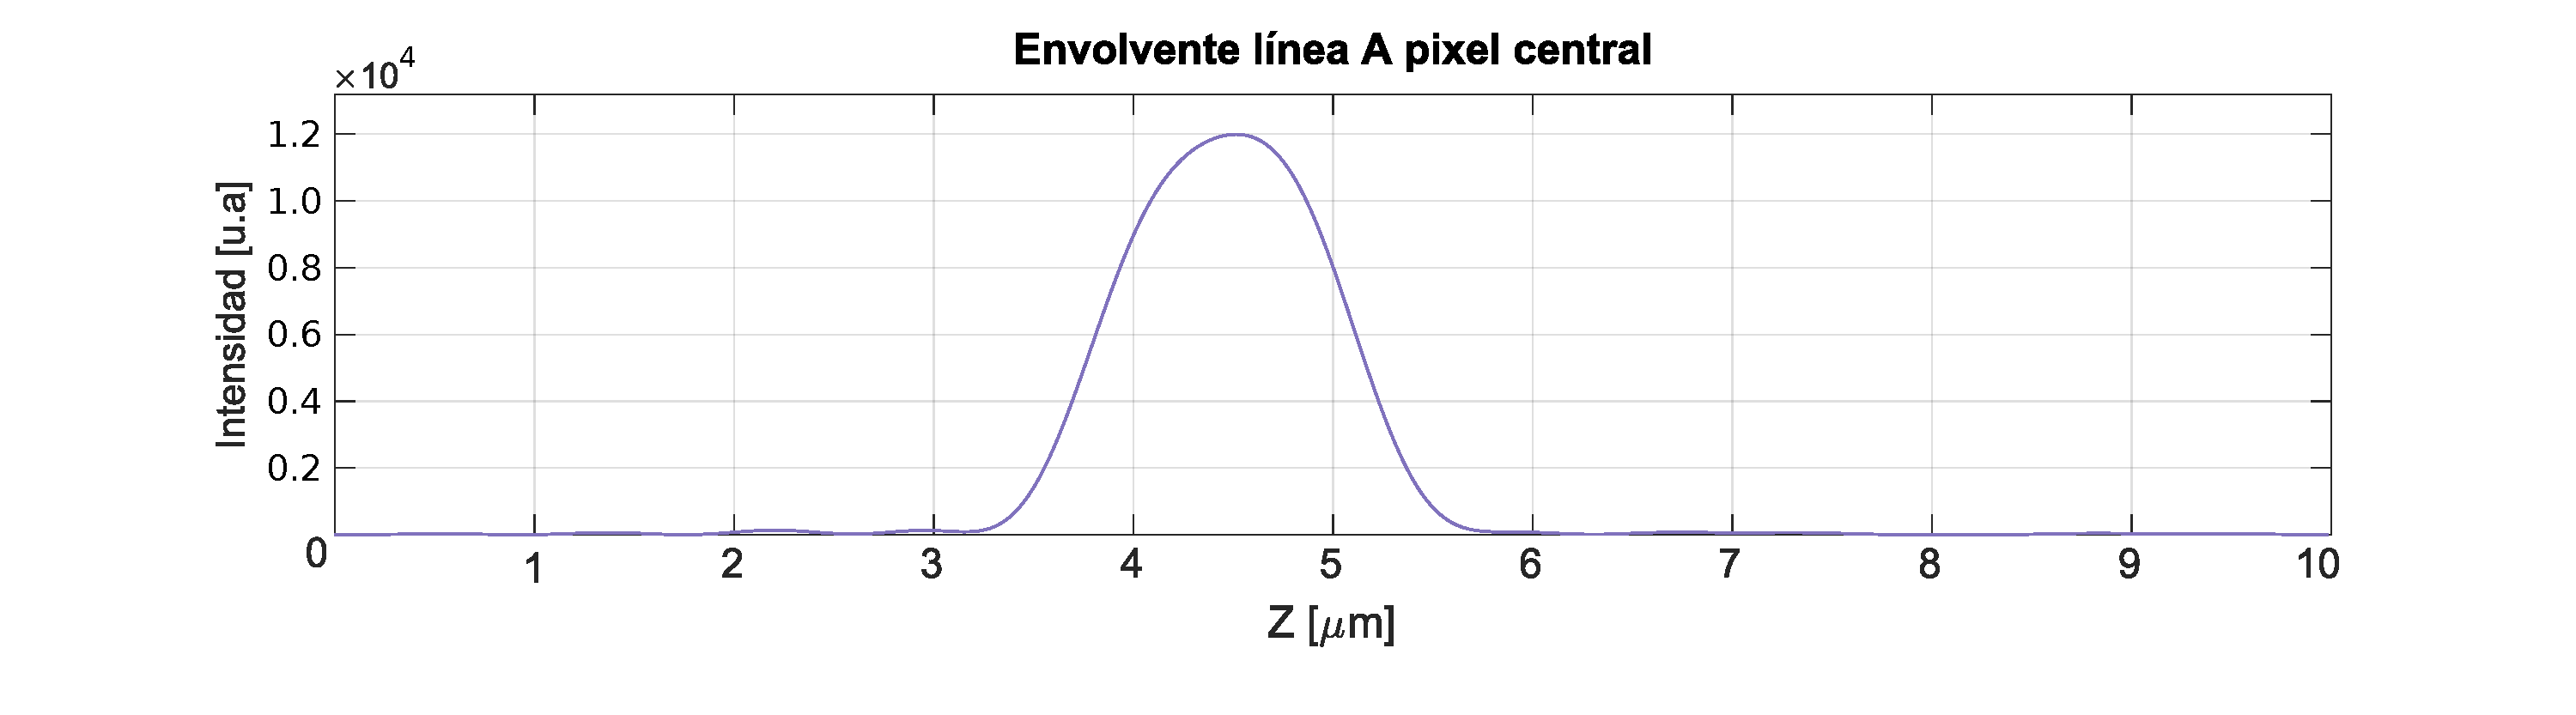
\includegraphics[width=8cm]{AAUgraphics/pt2/LineaAPXCenterEnvelop}
	\end{center}
	
\end{frame}

%%%%%%%%%%%%%%%%%%%%%%%%%%
%\subsubsection{Resultados obtenidos}
\begin{frame}{Sistema de OCT a nivel del laboratorio}{Resultados: Topografía de moneda}
	Guacamaya bandera
	\begin{center}
		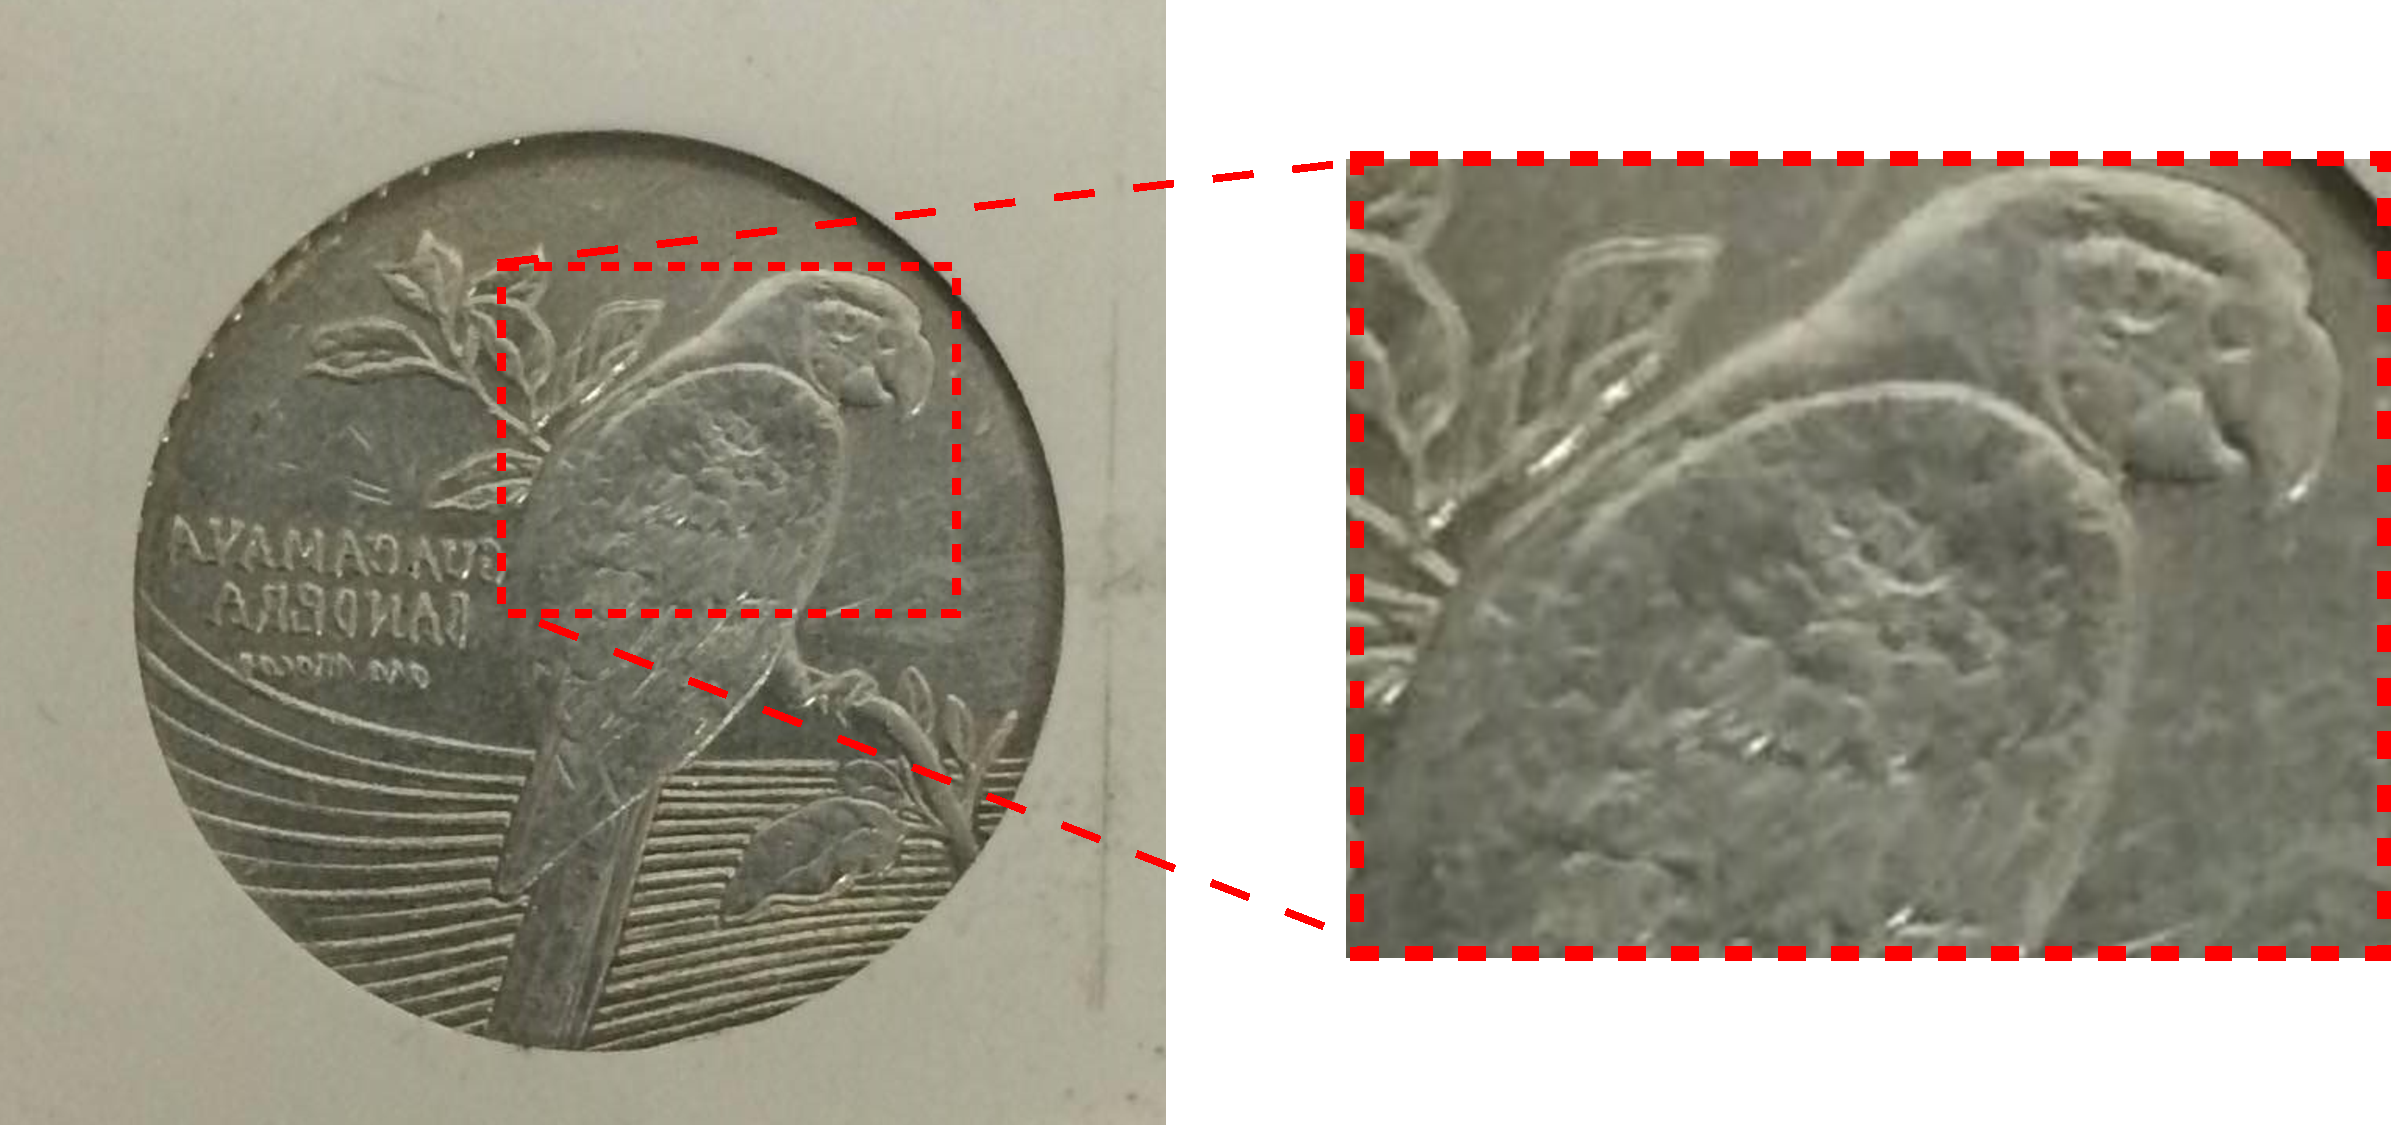
\includegraphics[width=1\linewidth]{AAUgraphics/pt2/Moneda_Directa_img}
	\end{center}
\end{frame}

%\begin{frame}{Sistema de OCT a nivel del laboratorio}{Topografía de moneda: Patrones capturados}
%	%Patrones interferencia capturados
%	
%	%\movie[width=4cm,height=4cm]{}{CoinEnfacegray.avi}
%	
%	%% OPCION 1 FUNCIONA
%	\begin{center}
%		\includegraphics[width=1\linewidth]
%			{AAUgraphics/pt2/Enface_Sequence}
%	\end{center}
%	
%\end{frame}

\begin{frame}{Sistema de OCT a nivel del laboratorio}{Topografía de moneda: Patrones de interferencia capturados}
	%\addtocounter{framenumber}{-1}
	\begin{center}
		\movie[width = \linewidth, height= 0.55\linewidth, loop, autostart, poster] {}{AAUmovies/Coin_En_face_gray.avi}
		%\href{run:}{
		%	\includegraphics[width=1\linewidth]
		%	{AAUgraphics/pt2/Enface_Sequence}}
	\end{center}
	
\end{frame}




\begin{frame}{Sistema de OCT a nivel del laboratorio}{Topografía de moneda: Comparación}
	%Comparación imágenes \emph{en-face}.
	
	\begin{multicols}{2}
		\centering
		%\hspace*{-0.75cm}
		Proyección \emph{en-face}
		
		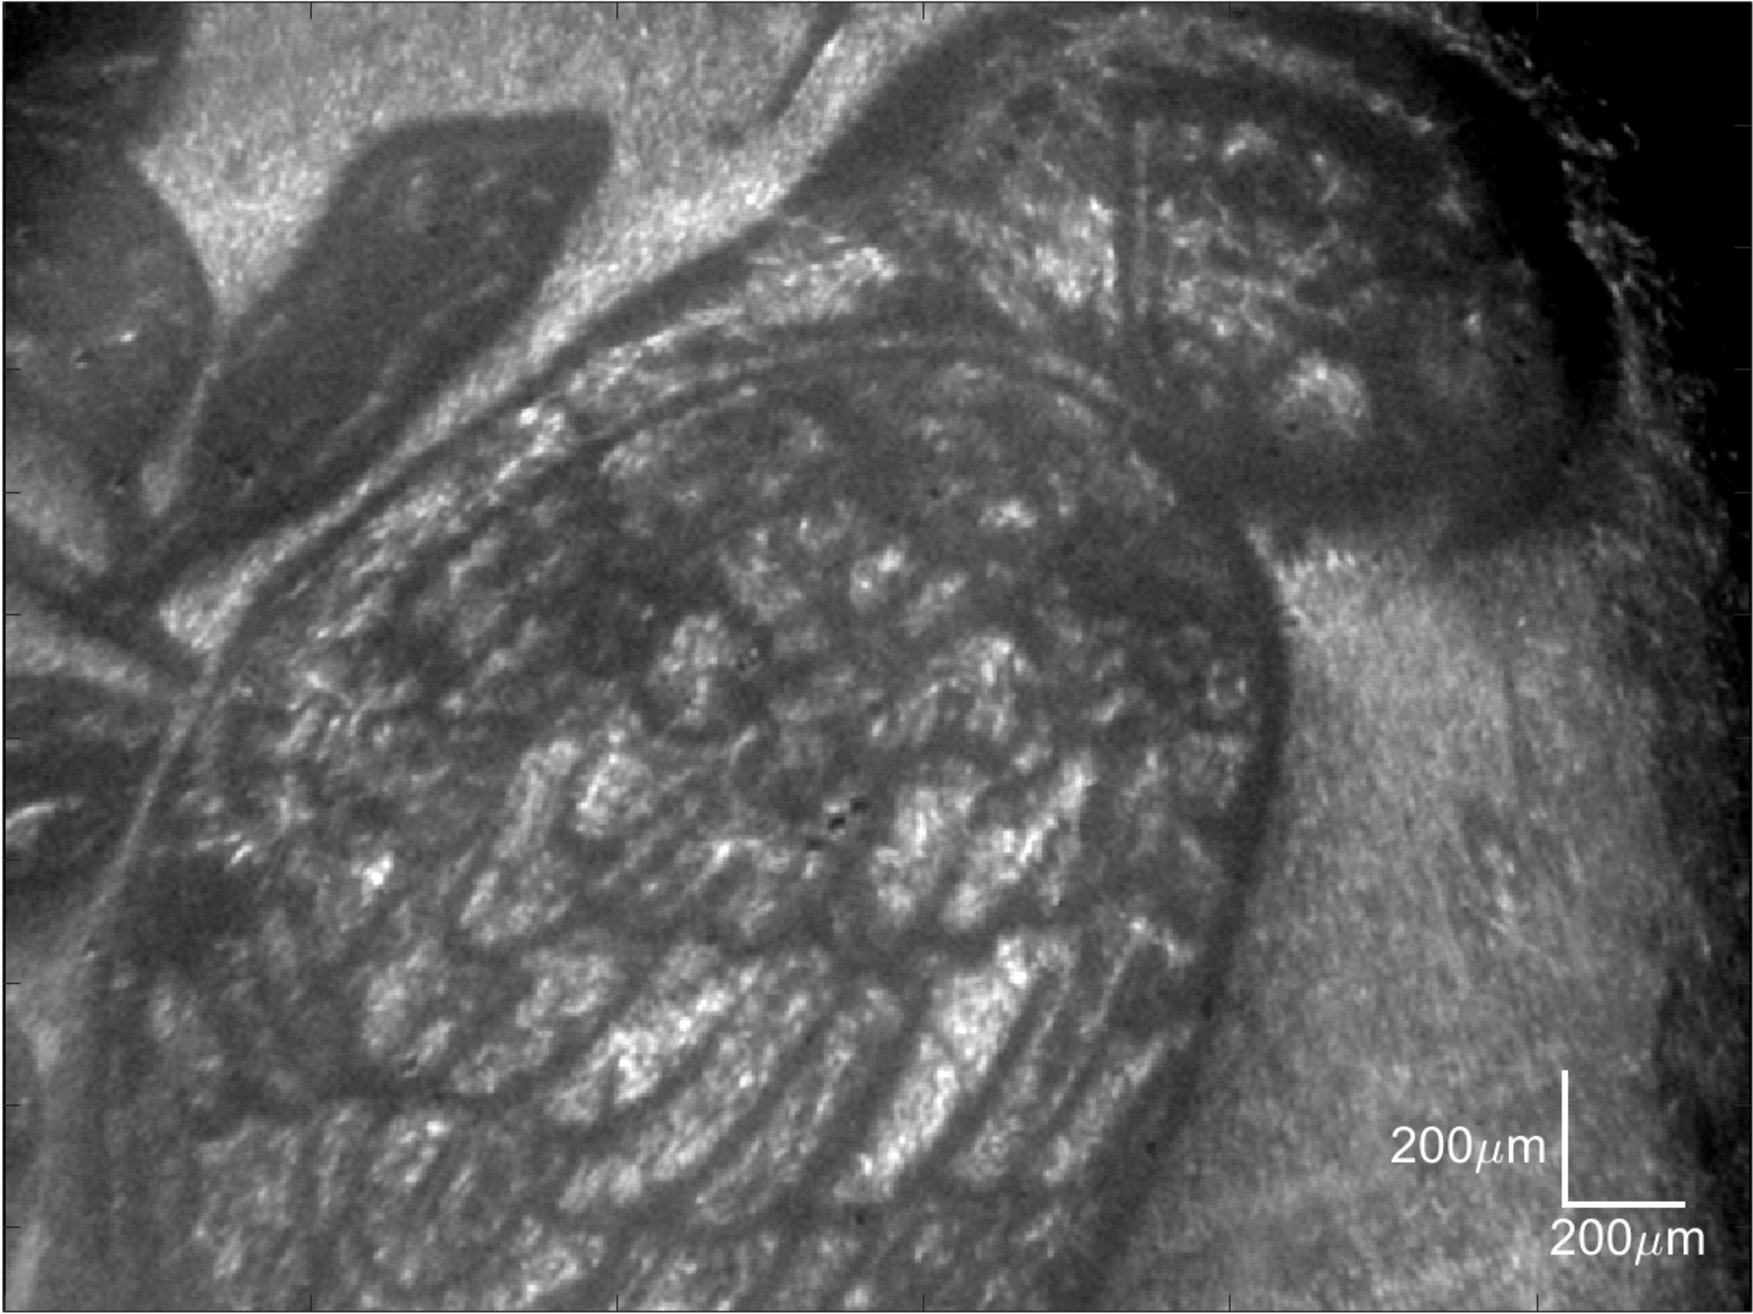
\includegraphics[width=1\linewidth]{AAUgraphics/pt2/OCT_En_face_Projection}
		\newpage
		%\vspace*{-0.22cm}
		
		Captura directa
		
		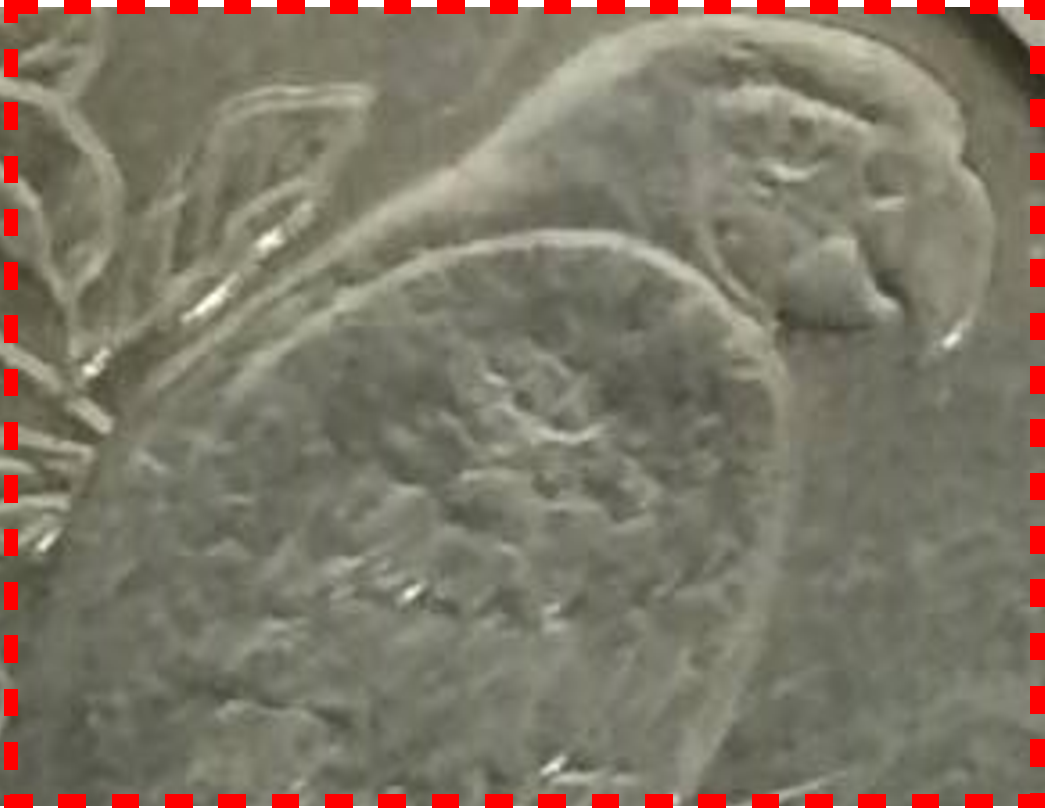
\includegraphics[width=0.98\linewidth]{AAUgraphics/pt2/Moneda_Directa_img_comparison}
	\end{multicols}
	
\end{frame}

%\begin{frame}{Sistema de OCT a nivel del laboratorio}{Resultados: Topografía de moneda}
%	Comparación imágenes en face
%	\begin{center}
%		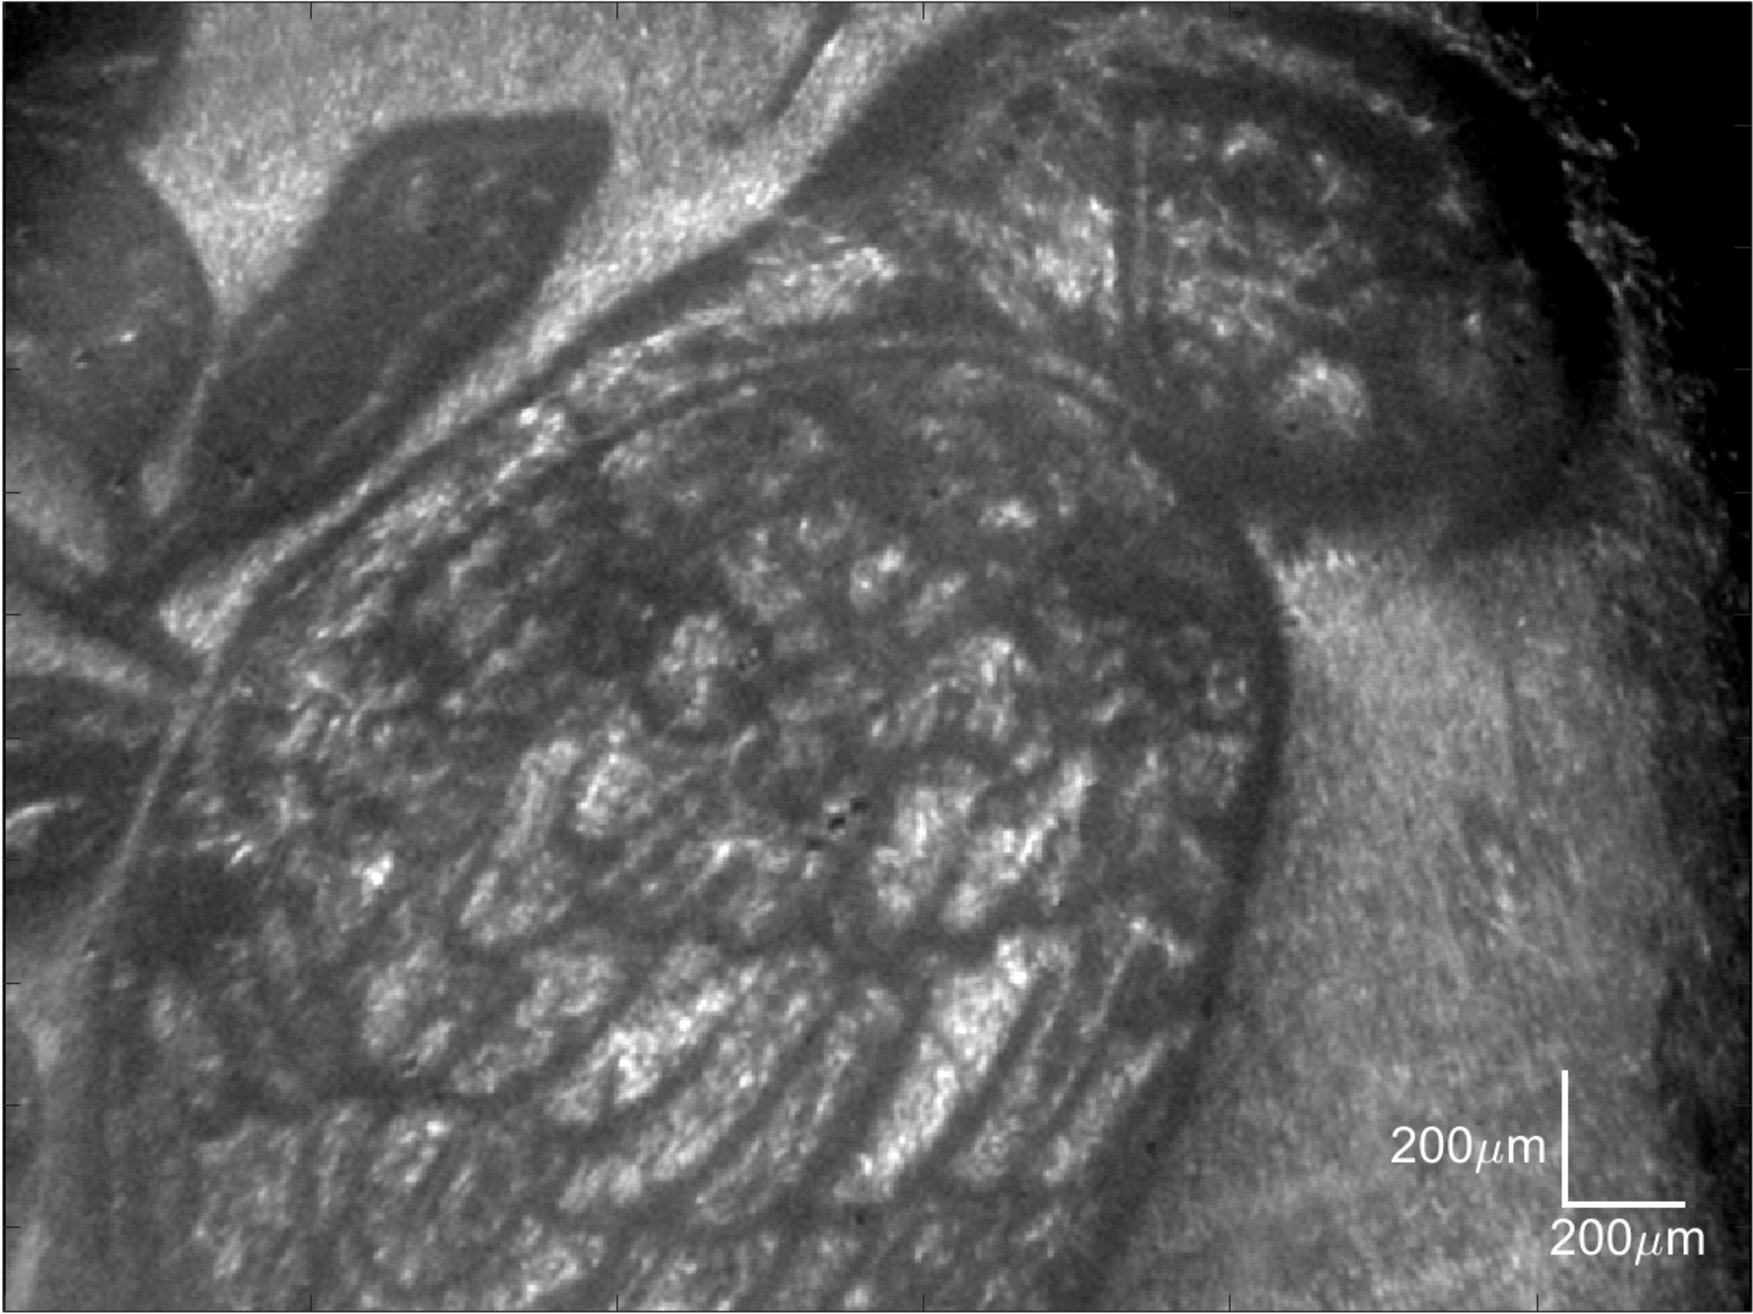
\includegraphics[width=0.7\linewidth]{AAUgraphics/pt2/OCT_En_face_Projection}
%	\end{center}
%	FALTA IMAGEN MONEDA COMPARACION
%\end{frame}

\begin{frame}{Sistema de OCT a nivel del laboratorio}{Topografía de moneda: Sección transversal}
	\centering
%	\href{run:AAUmovies/Coin_BScan_with_line.avi}{
%		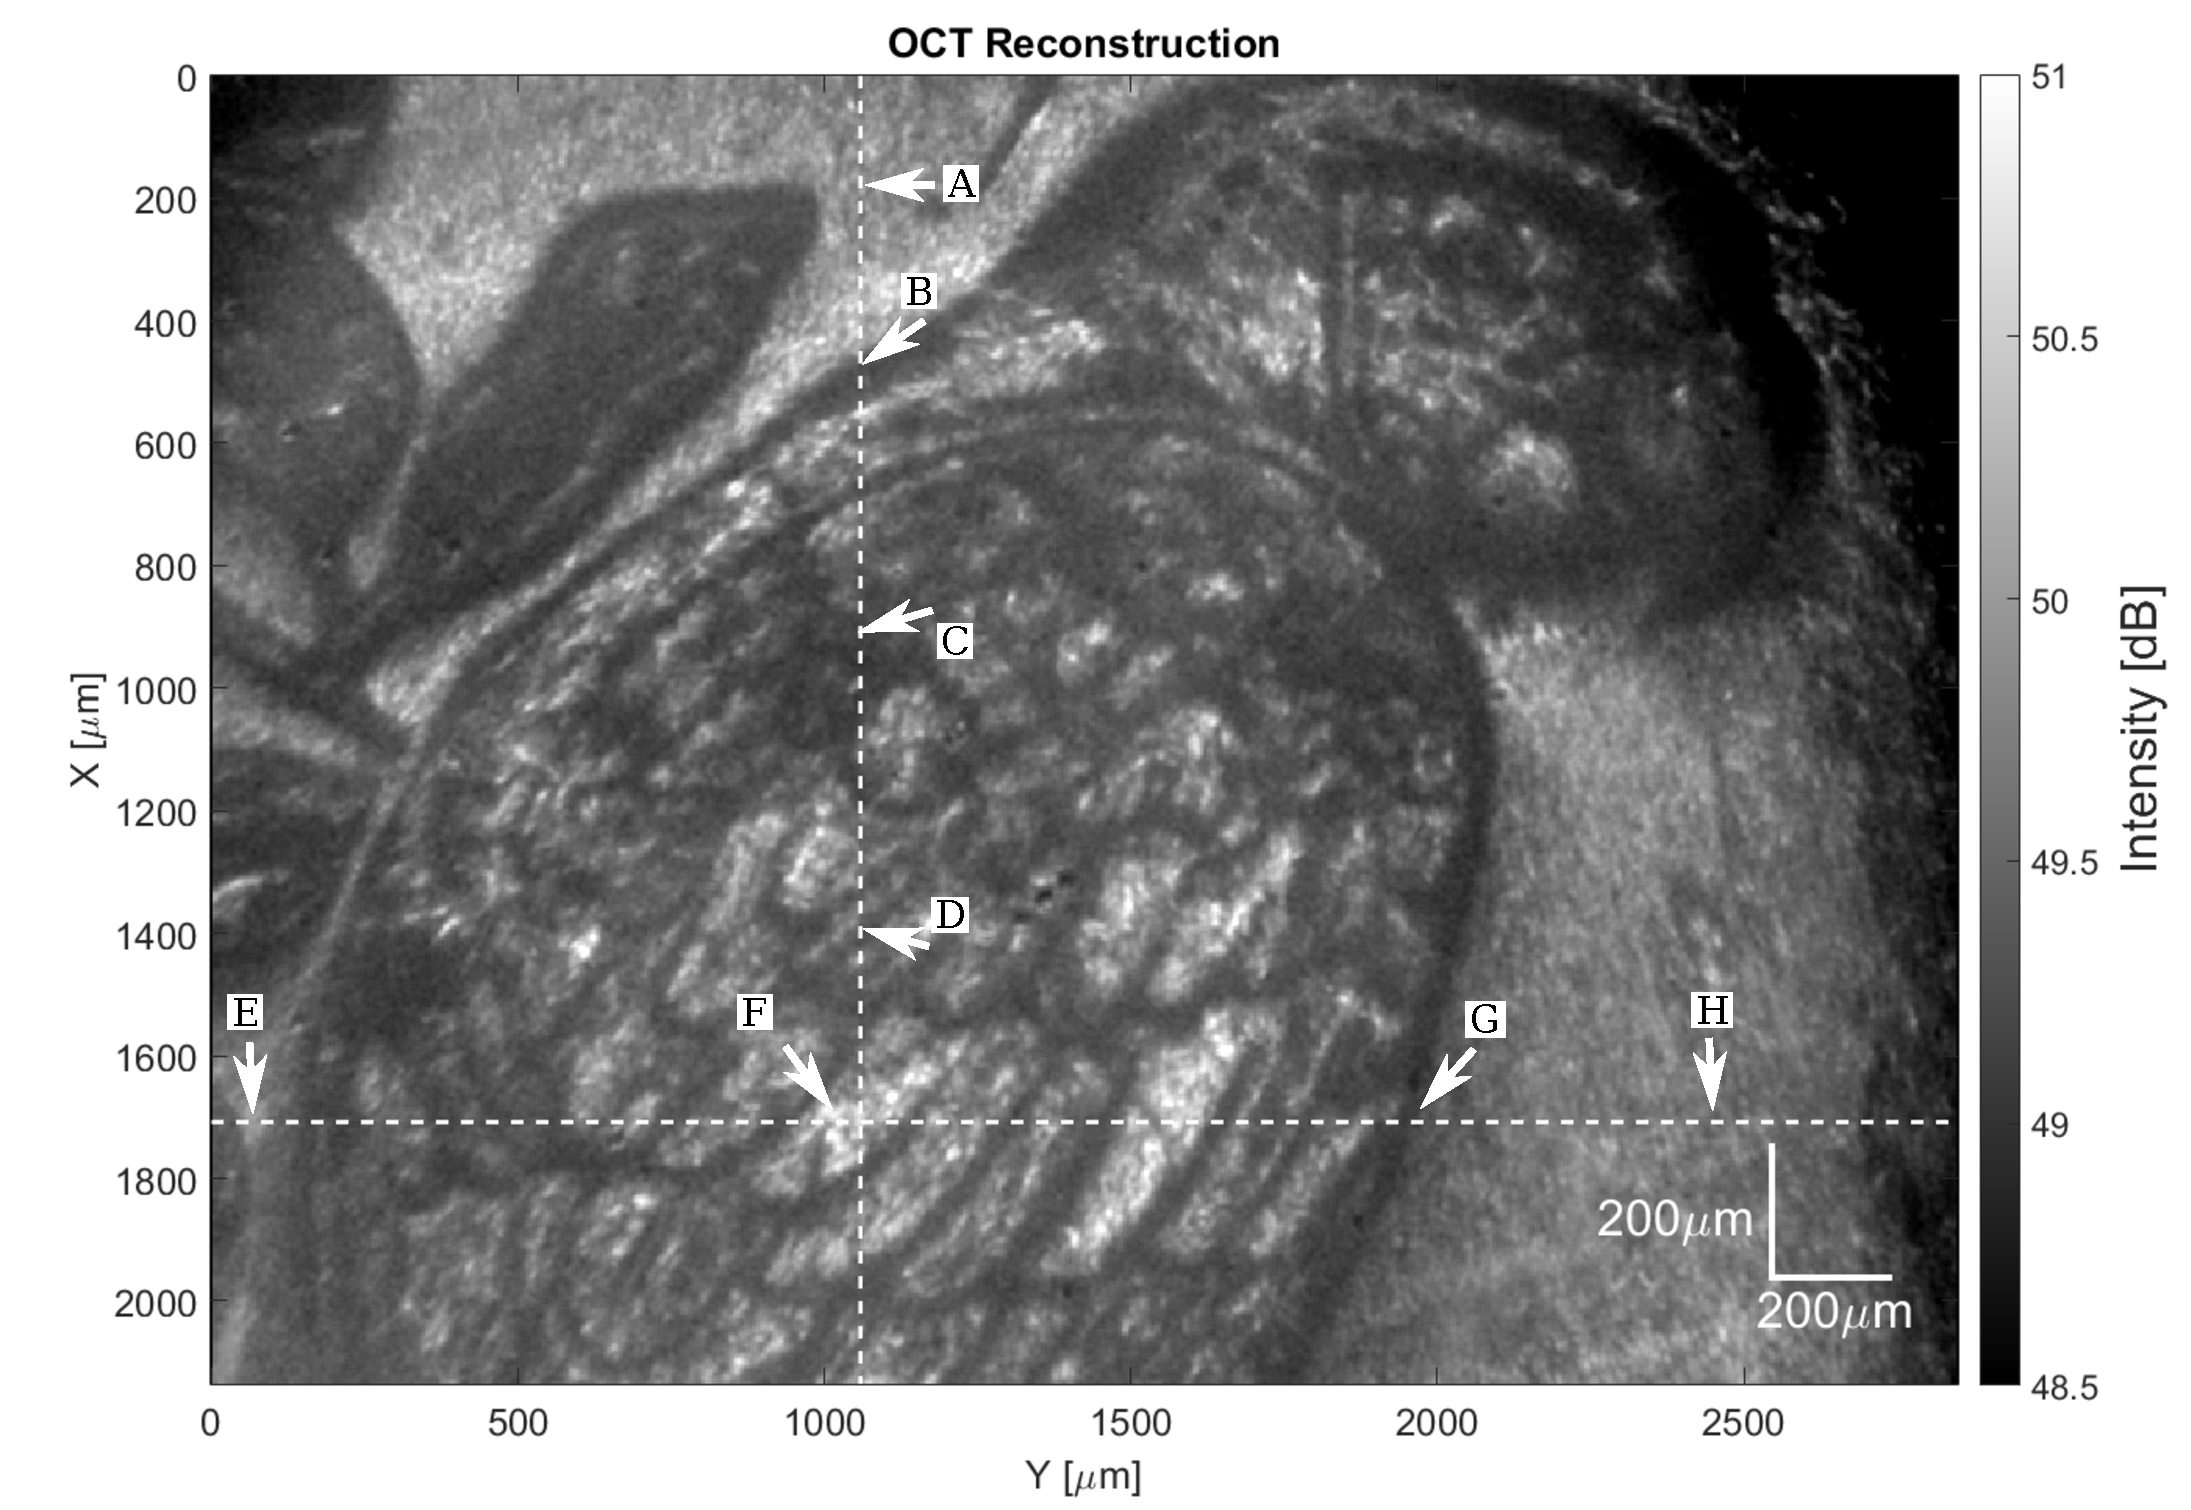
\includegraphics[width=0.49\linewidth]{AAUgraphics/pt2/OCT_Reconstruction_Moneda}}
	\vspace*{-0.1cm}
	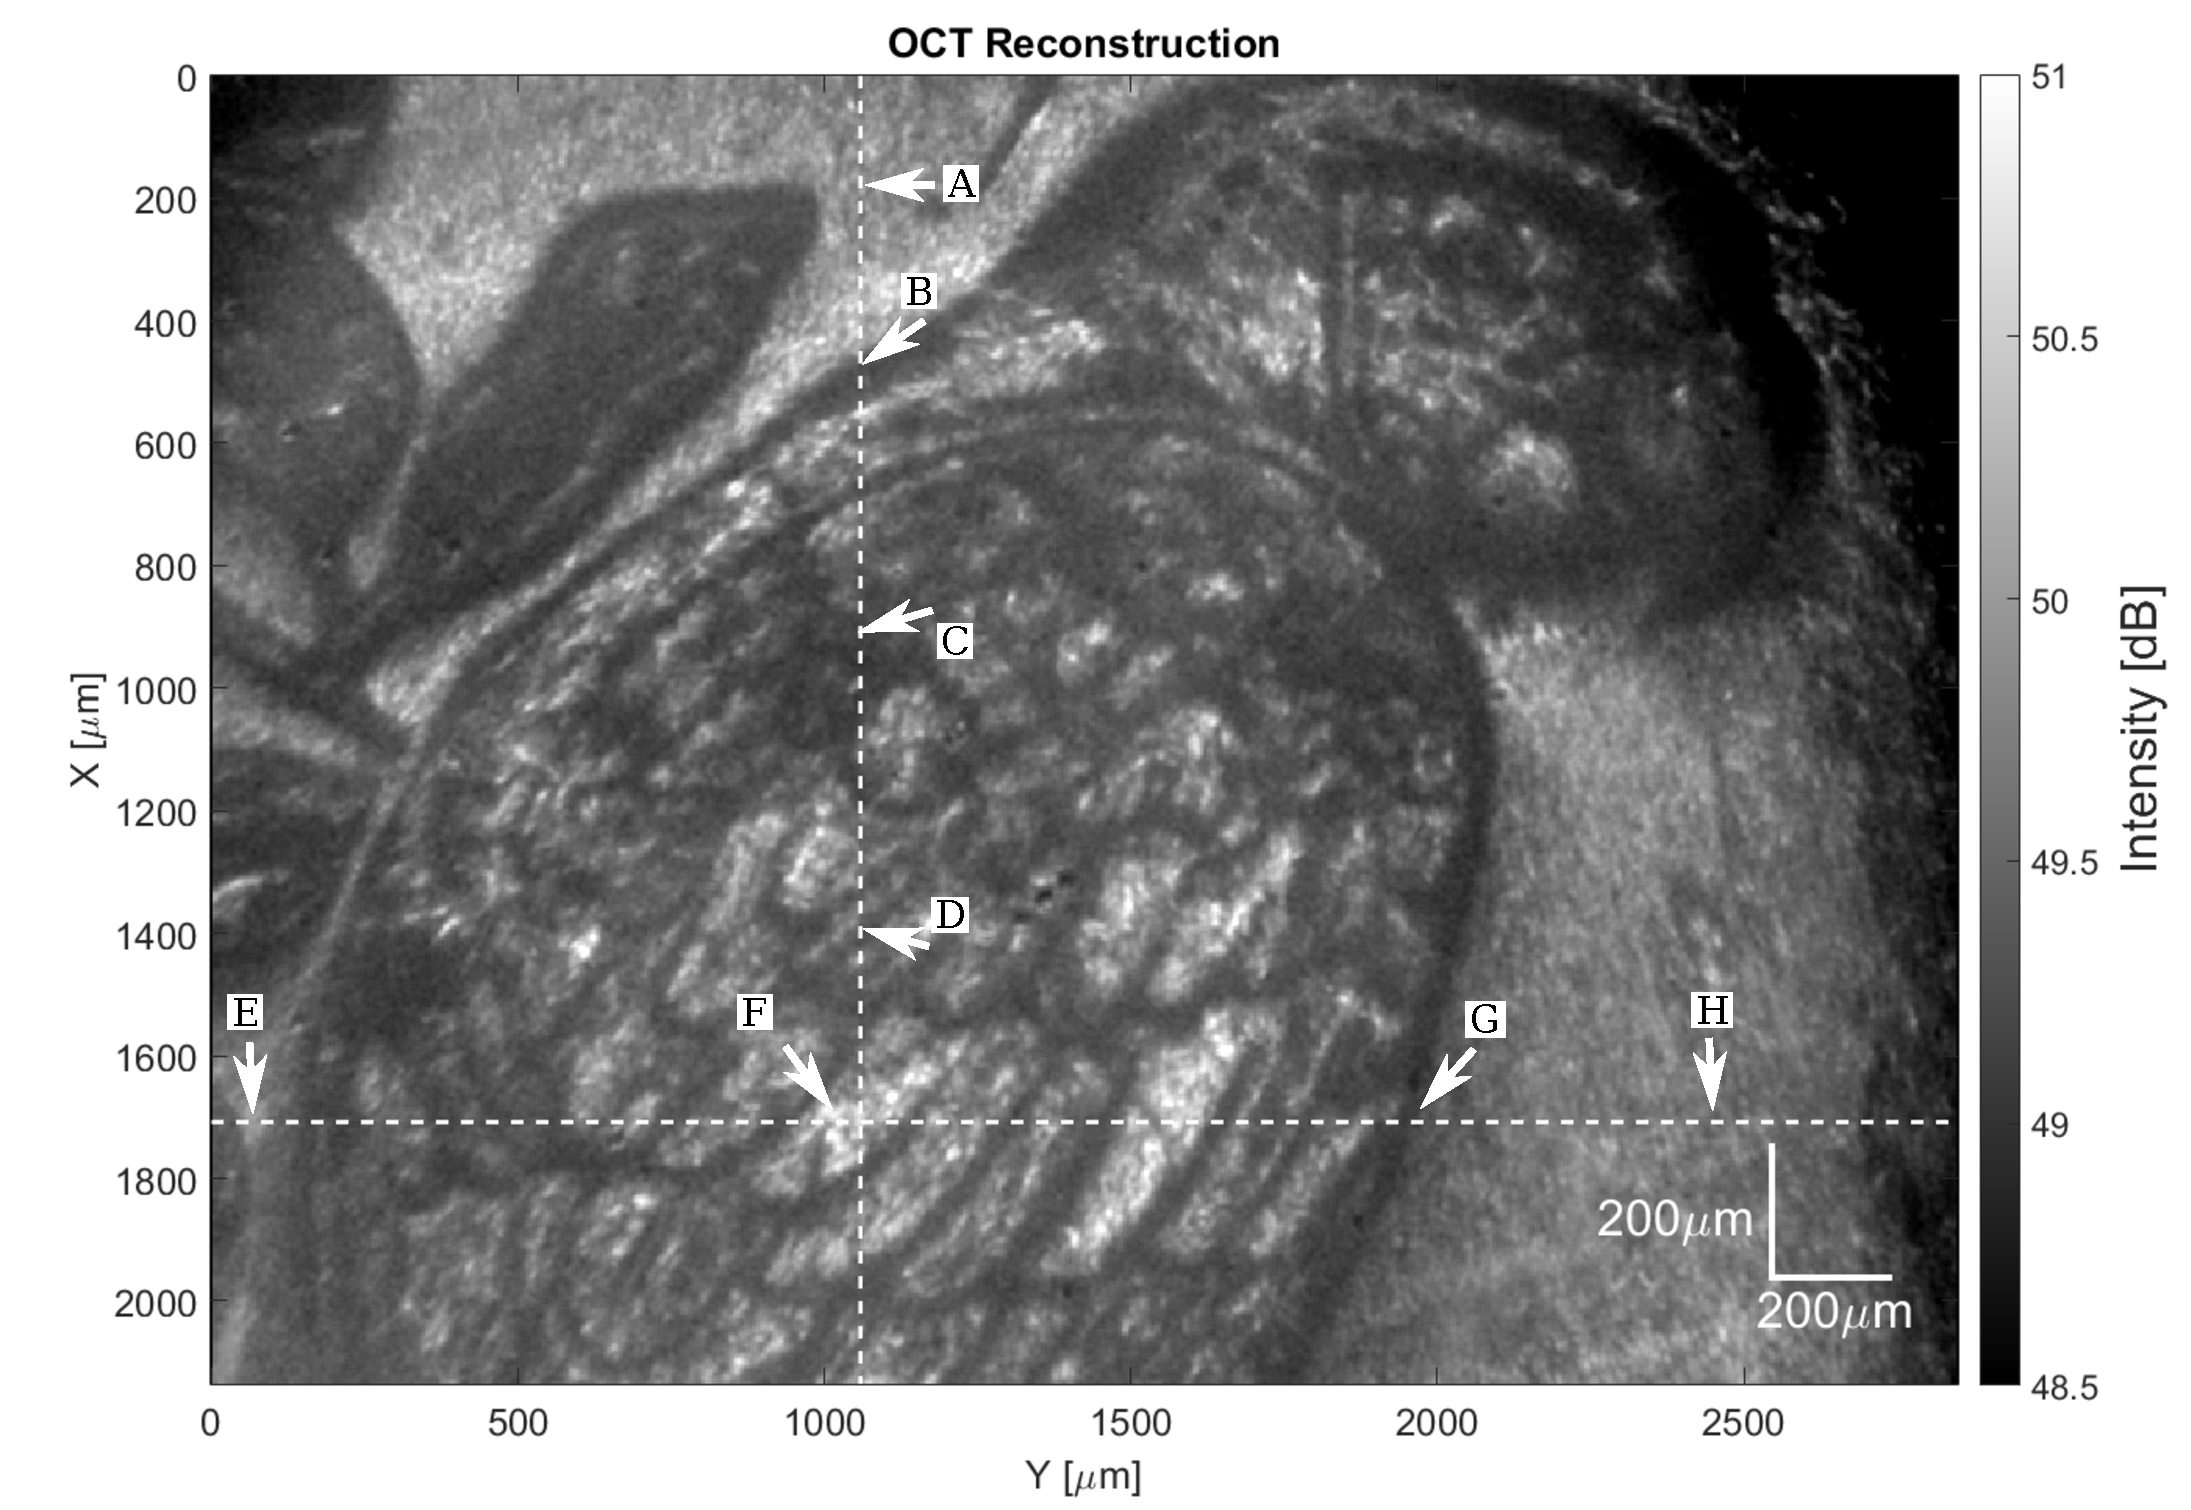
\includegraphics[width=0.7\linewidth]{AAUgraphics/pt2/OCT_Reconstruction_Moneda}
	
	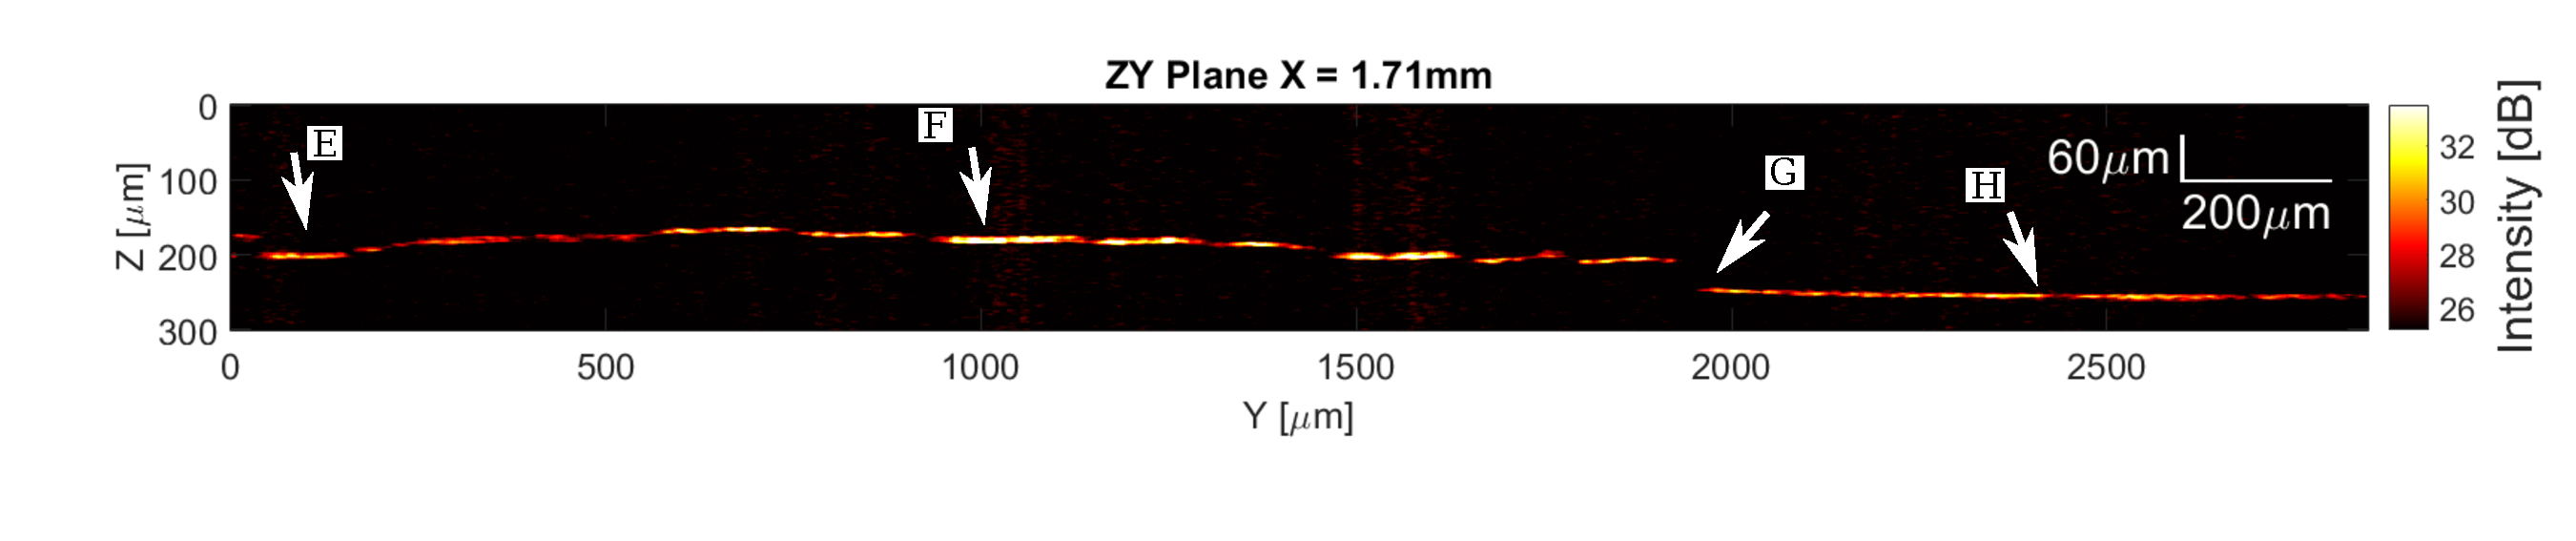
\includegraphics[width=8.2cm]{AAUgraphics/pt2/ZYPlane_moneda}

	\vspace*{-0.3cm}
	\hspace*{0.3cm}
	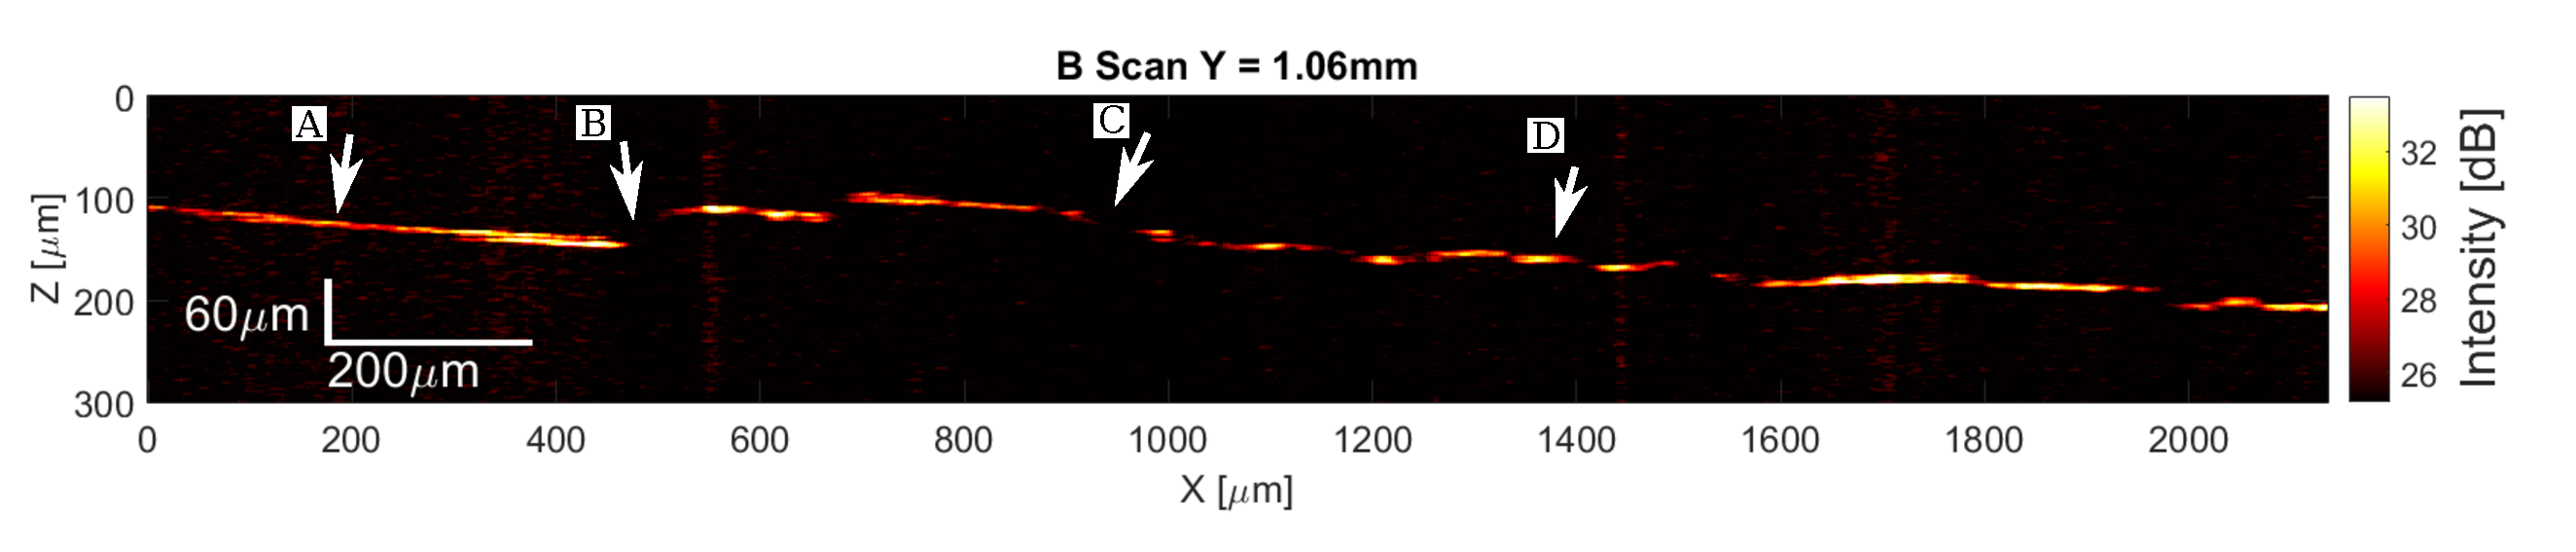
\includegraphics[width=8cm]{AAUgraphics/pt2/Bscan_Moneda}
\end{frame}

\begin{frame}{Sistema de OCT a nivel del laboratorio}{Topografía de moneda: Sección transversal}
	%\addtocounter{framenumber}{-1}
	
	
	\begin{center}
		\movie[width = \linewidth, height= 0.55\linewidth, loop, autostart, poster] {}{AAUmovies/Coin_BScan_with_line.avi}
		%\href{run:}{
		%	\includegraphics[width=1\linewidth]
		%	{AAUgraphics/pt2/Enface_Sequence}}
	\end{center}
\end{frame}
	

\begin{frame}{Sistema de OCT a nivel del laboratorio}{Topografía de moneda: Renderizado}
	%\centering
%	\href{run:AAUmovies/Coin_Guacamaya3D_Slow_motion.avi}{
%		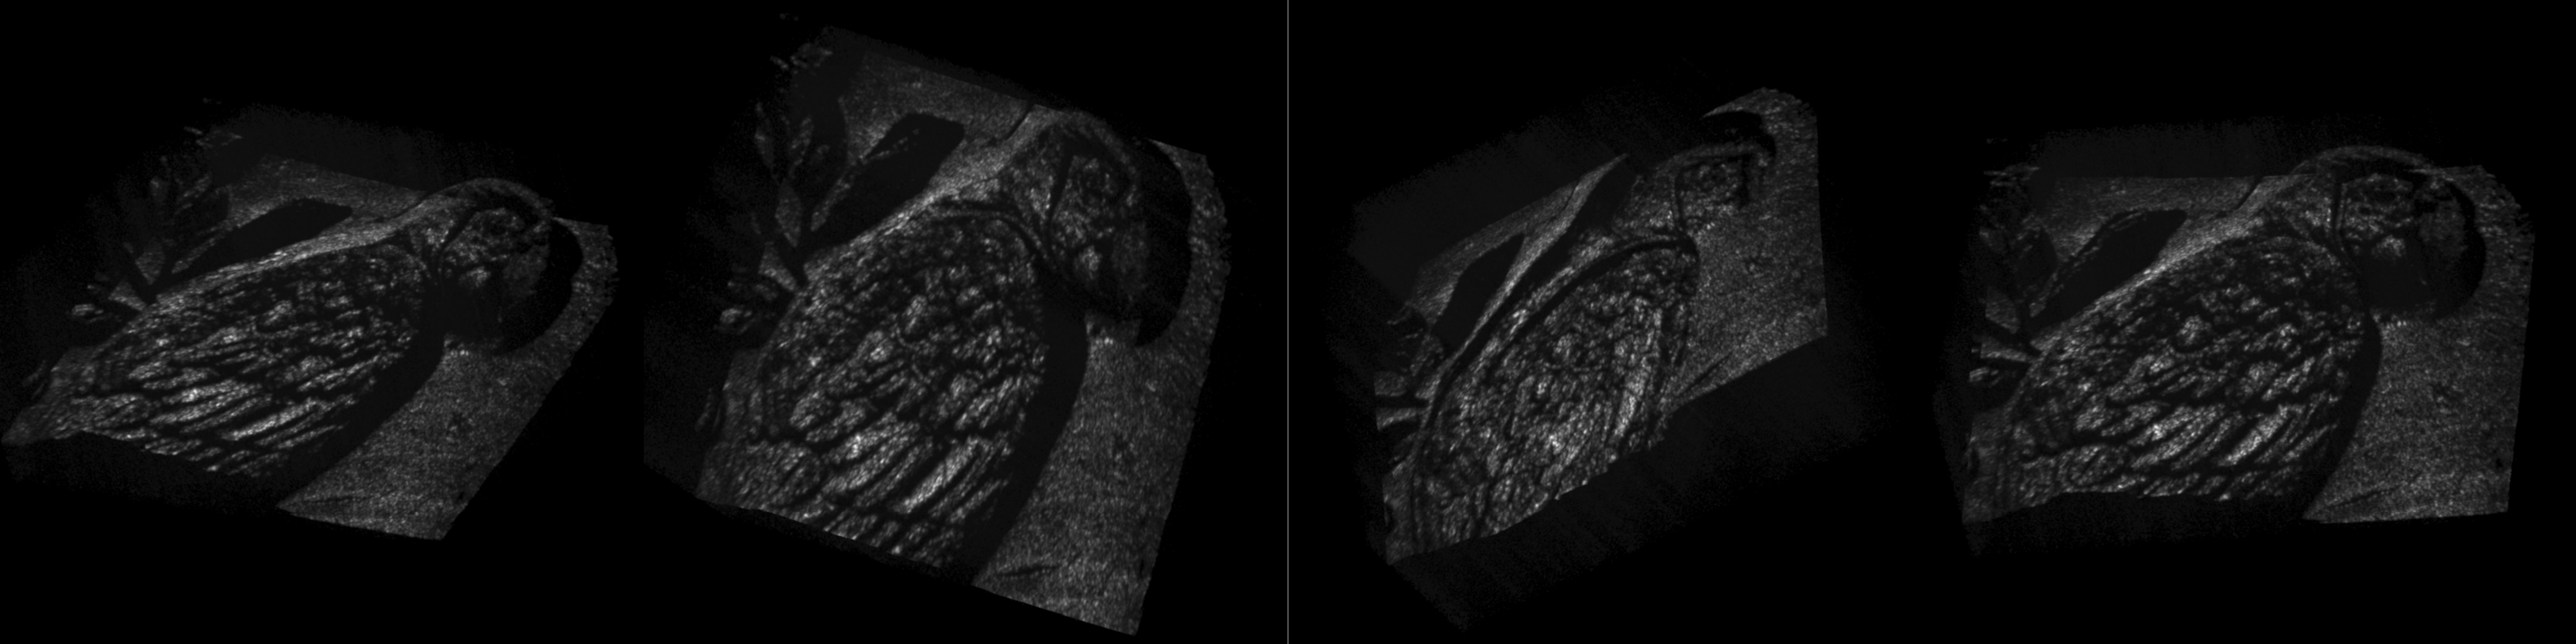
\includegraphics[width=1\linewidth]{AAUgraphics/pt2/PerspectivasTopologia}}
	\movie[width = \linewidth, height= 0.55\linewidth, loop, autostart, poster] {}{AAUmovies/Coin_Guacamaya3D_Slow_motion.avi}
	
\end{frame}


%%%%%%%%%%%%%%%%%%%%%%%%%%
%\subsubsection{Resultados obtenidos}
\begin{frame}{Sistema de OCT a nivel del laboratorio}{Resultados: Estructura ala de \emph{blattodea} (\emph{tegmen})}
	\blfootnote{{\tiny \url{http://www.godofinsects.com/files/6912/7632/8403/166_12.jpg}}}
	{\centering
	\emph{Blattodea}
	
	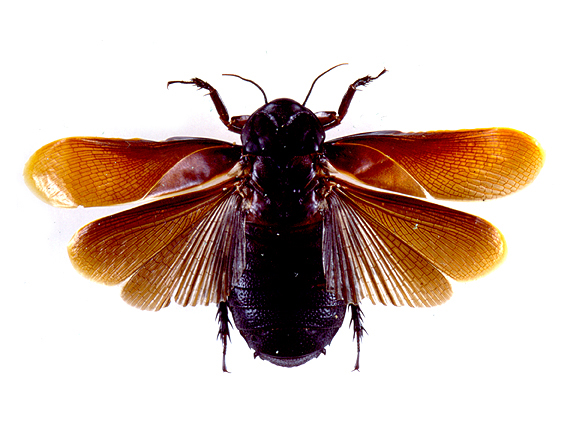
\includegraphics[width=0.4\linewidth]{AAUgraphics/pt2/166_12} \par}
	
	Muestra del insecto
	
	{\centering
	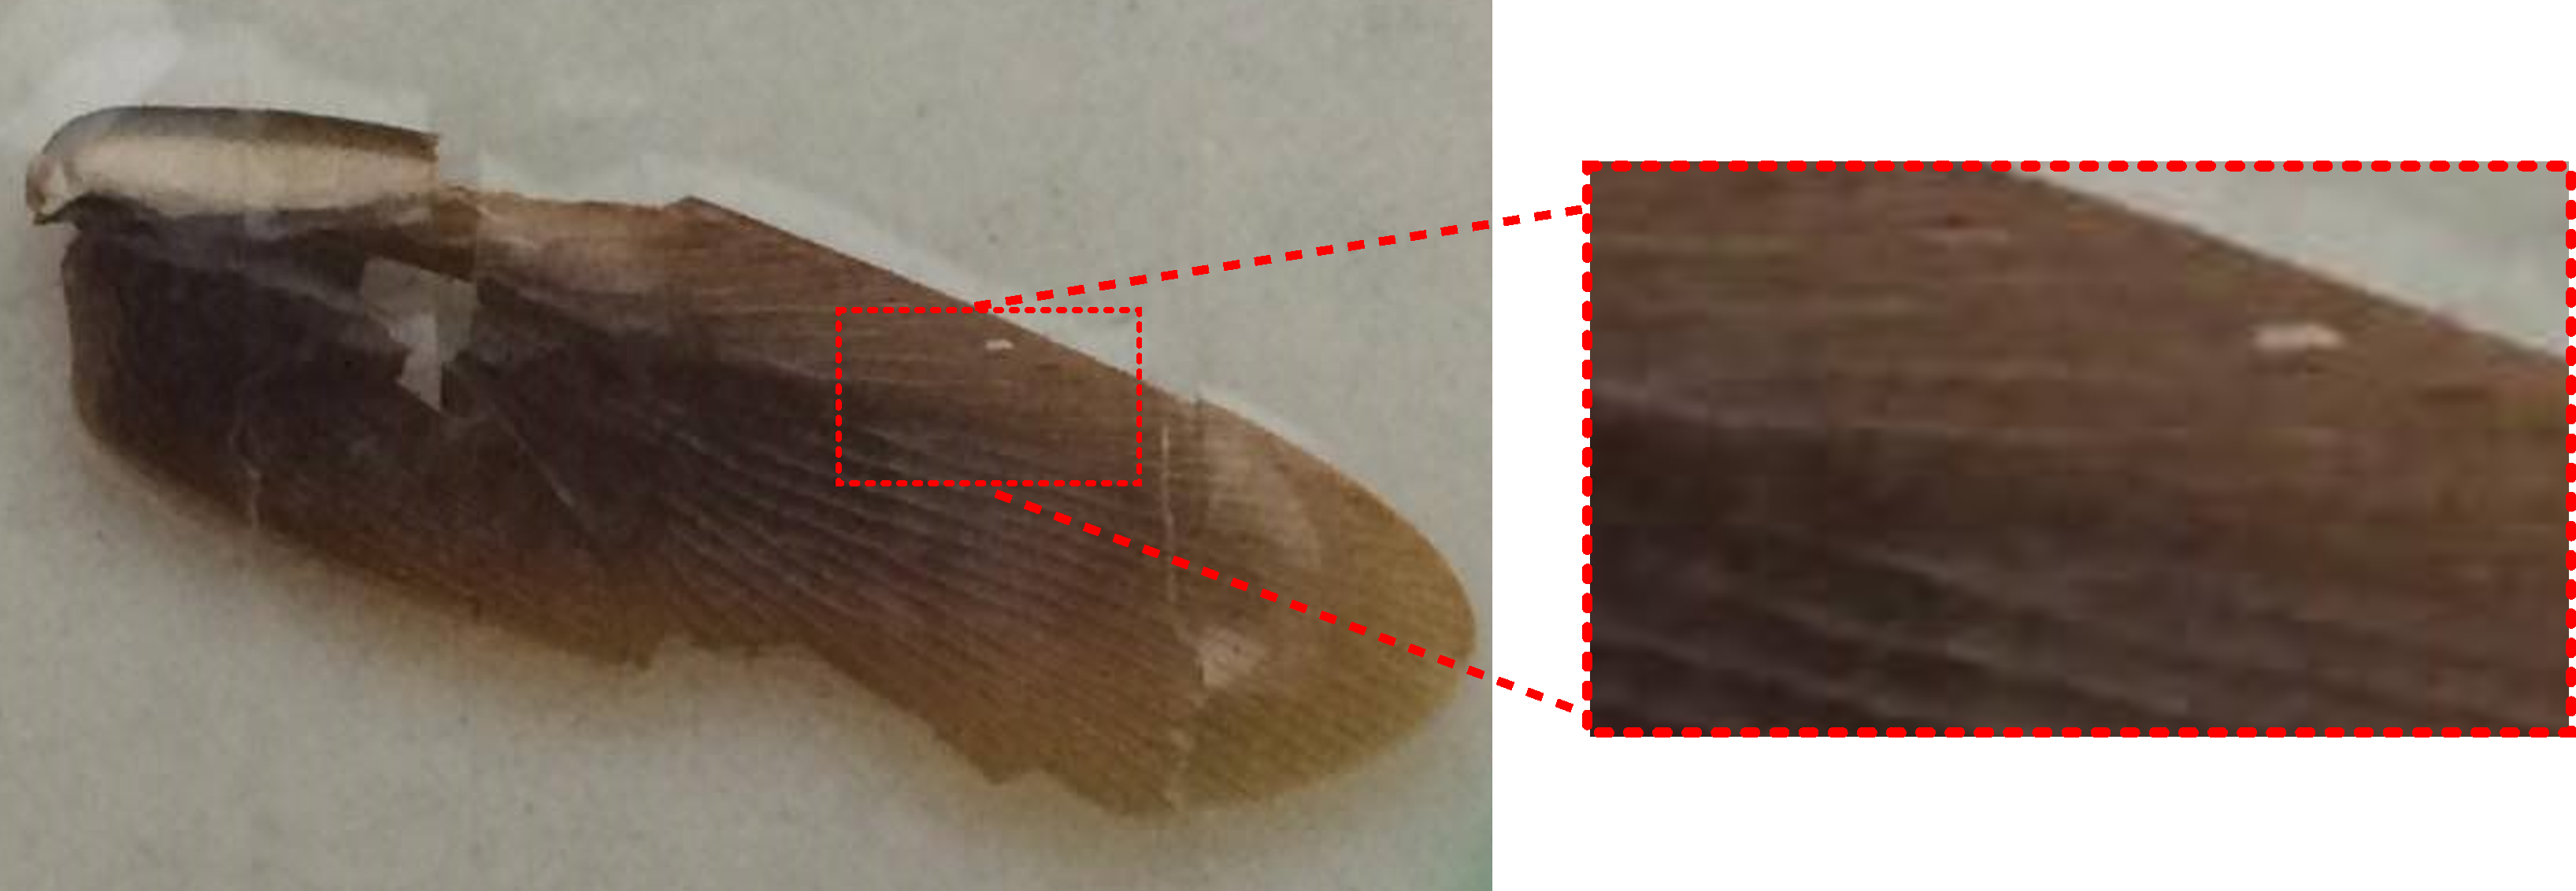
\includegraphics[width=1\linewidth]{AAUgraphics/pt2/BlattoaWingZoomed}}
\end{frame}

\begin{frame}{Sistema de OCT a nivel del laboratorio}{Estructura ala de \emph{blattodea}: Patrones de interferencia capturados}
	%Patrones interferencia capturados
	
	\vfill
	\begin{center}
		\movie[width = \linewidth, height= 0.55\linewidth, loop, autostart, poster] {}{AAUmovies/Blattodea_En_face.avi}
		%\href{run:AAUmovies/Blattodea_En_face.avi}{
		%	\includegraphics[width=1\linewidth]
		%	{AAUgraphics/pt2/Wing_Enface_cover.pdf}}
	\end{center}
\end{frame}

\begin{frame}{Sistema de OCT a nivel del laboratorio}{Estructura ala de \emph{blattodea}: Comparación}
	%Comparación imágenes \emph{en-face}.
		
	\begin{multicols}{2}
			\centering
			%\hspace*{-0.5cm}
			Proyección \emph{en-face}
			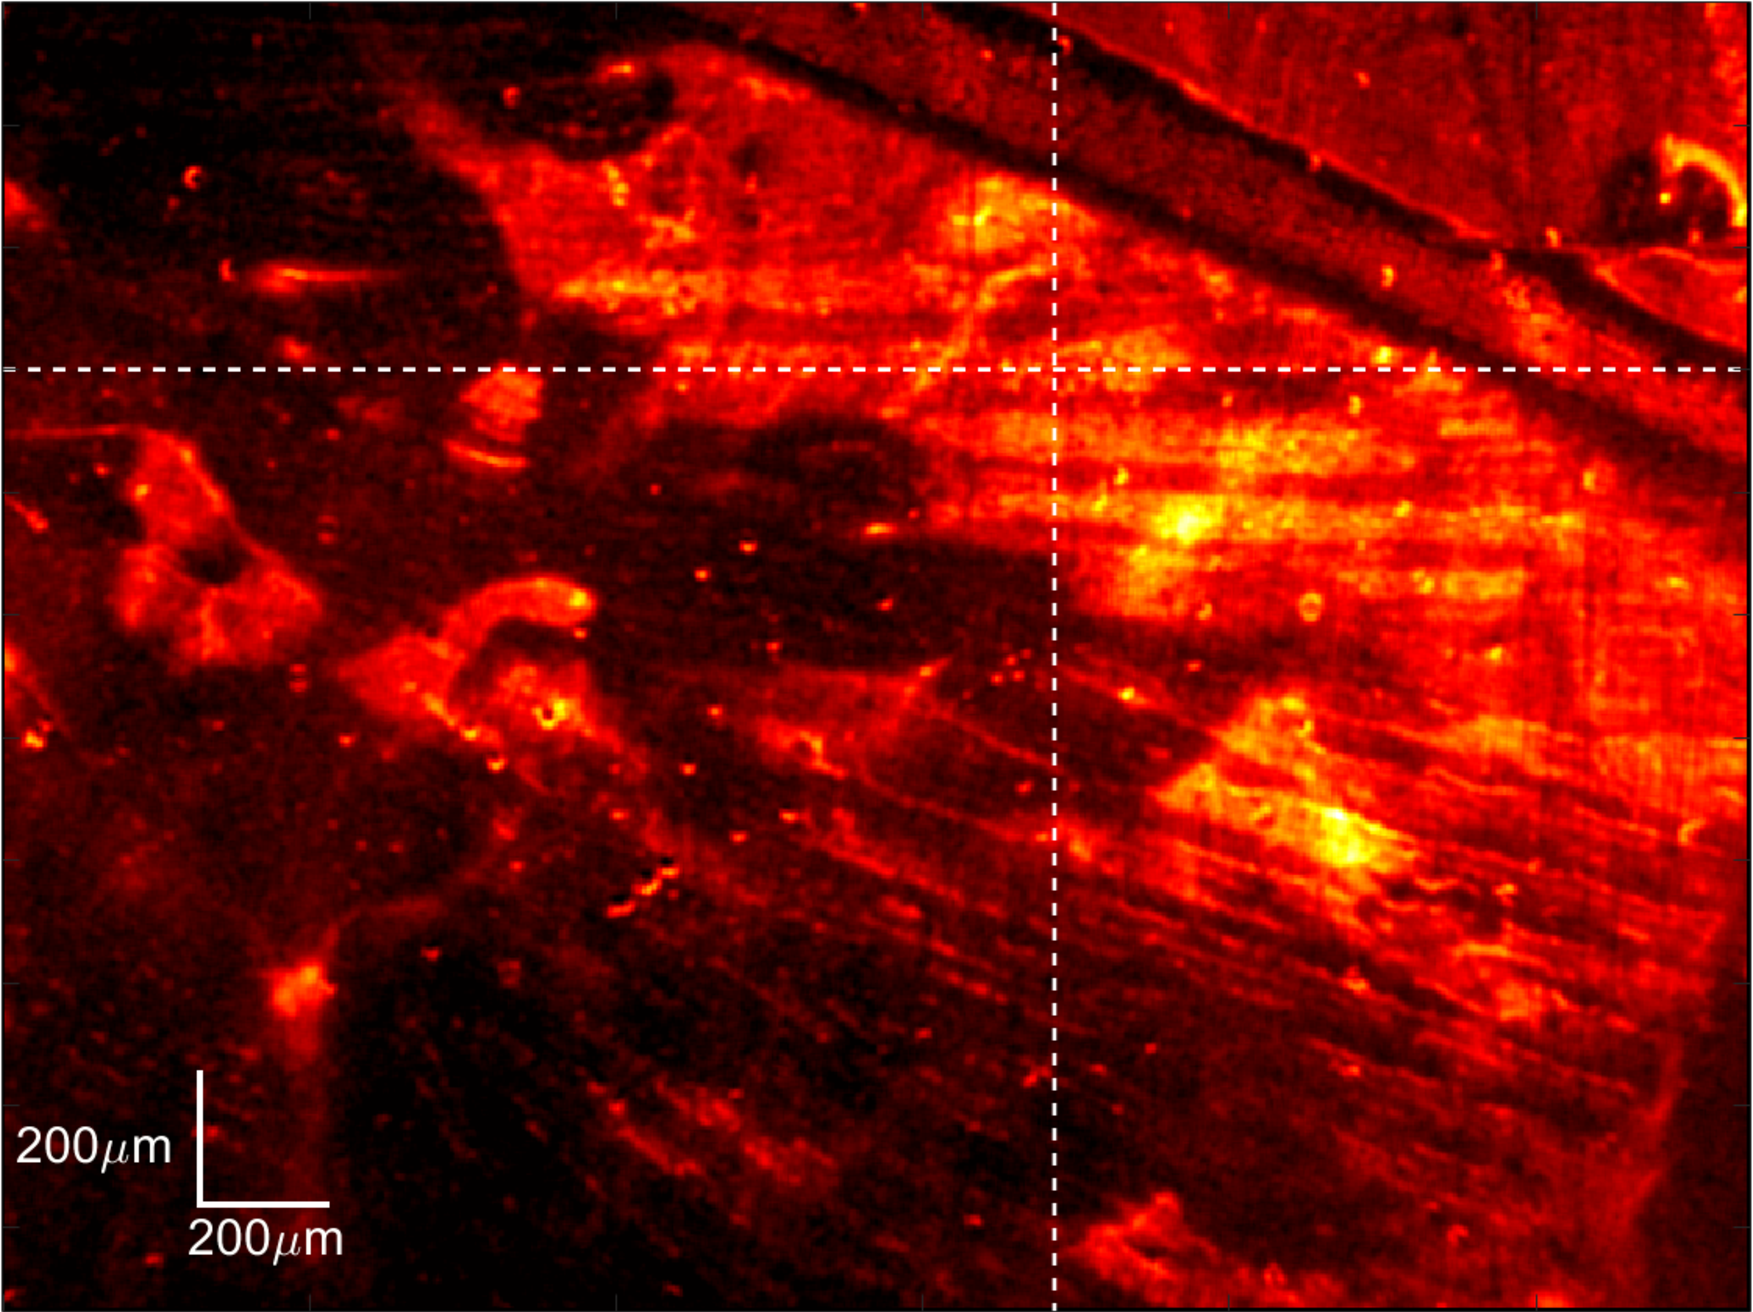
\includegraphics[width=1\linewidth]{AAUgraphics/pt2/OCT_Reconstruction_wing}
			\newpage
			
			Captura directa
			%\hspace*{0.1cm}
			%\vspace*{-1.22cm}
			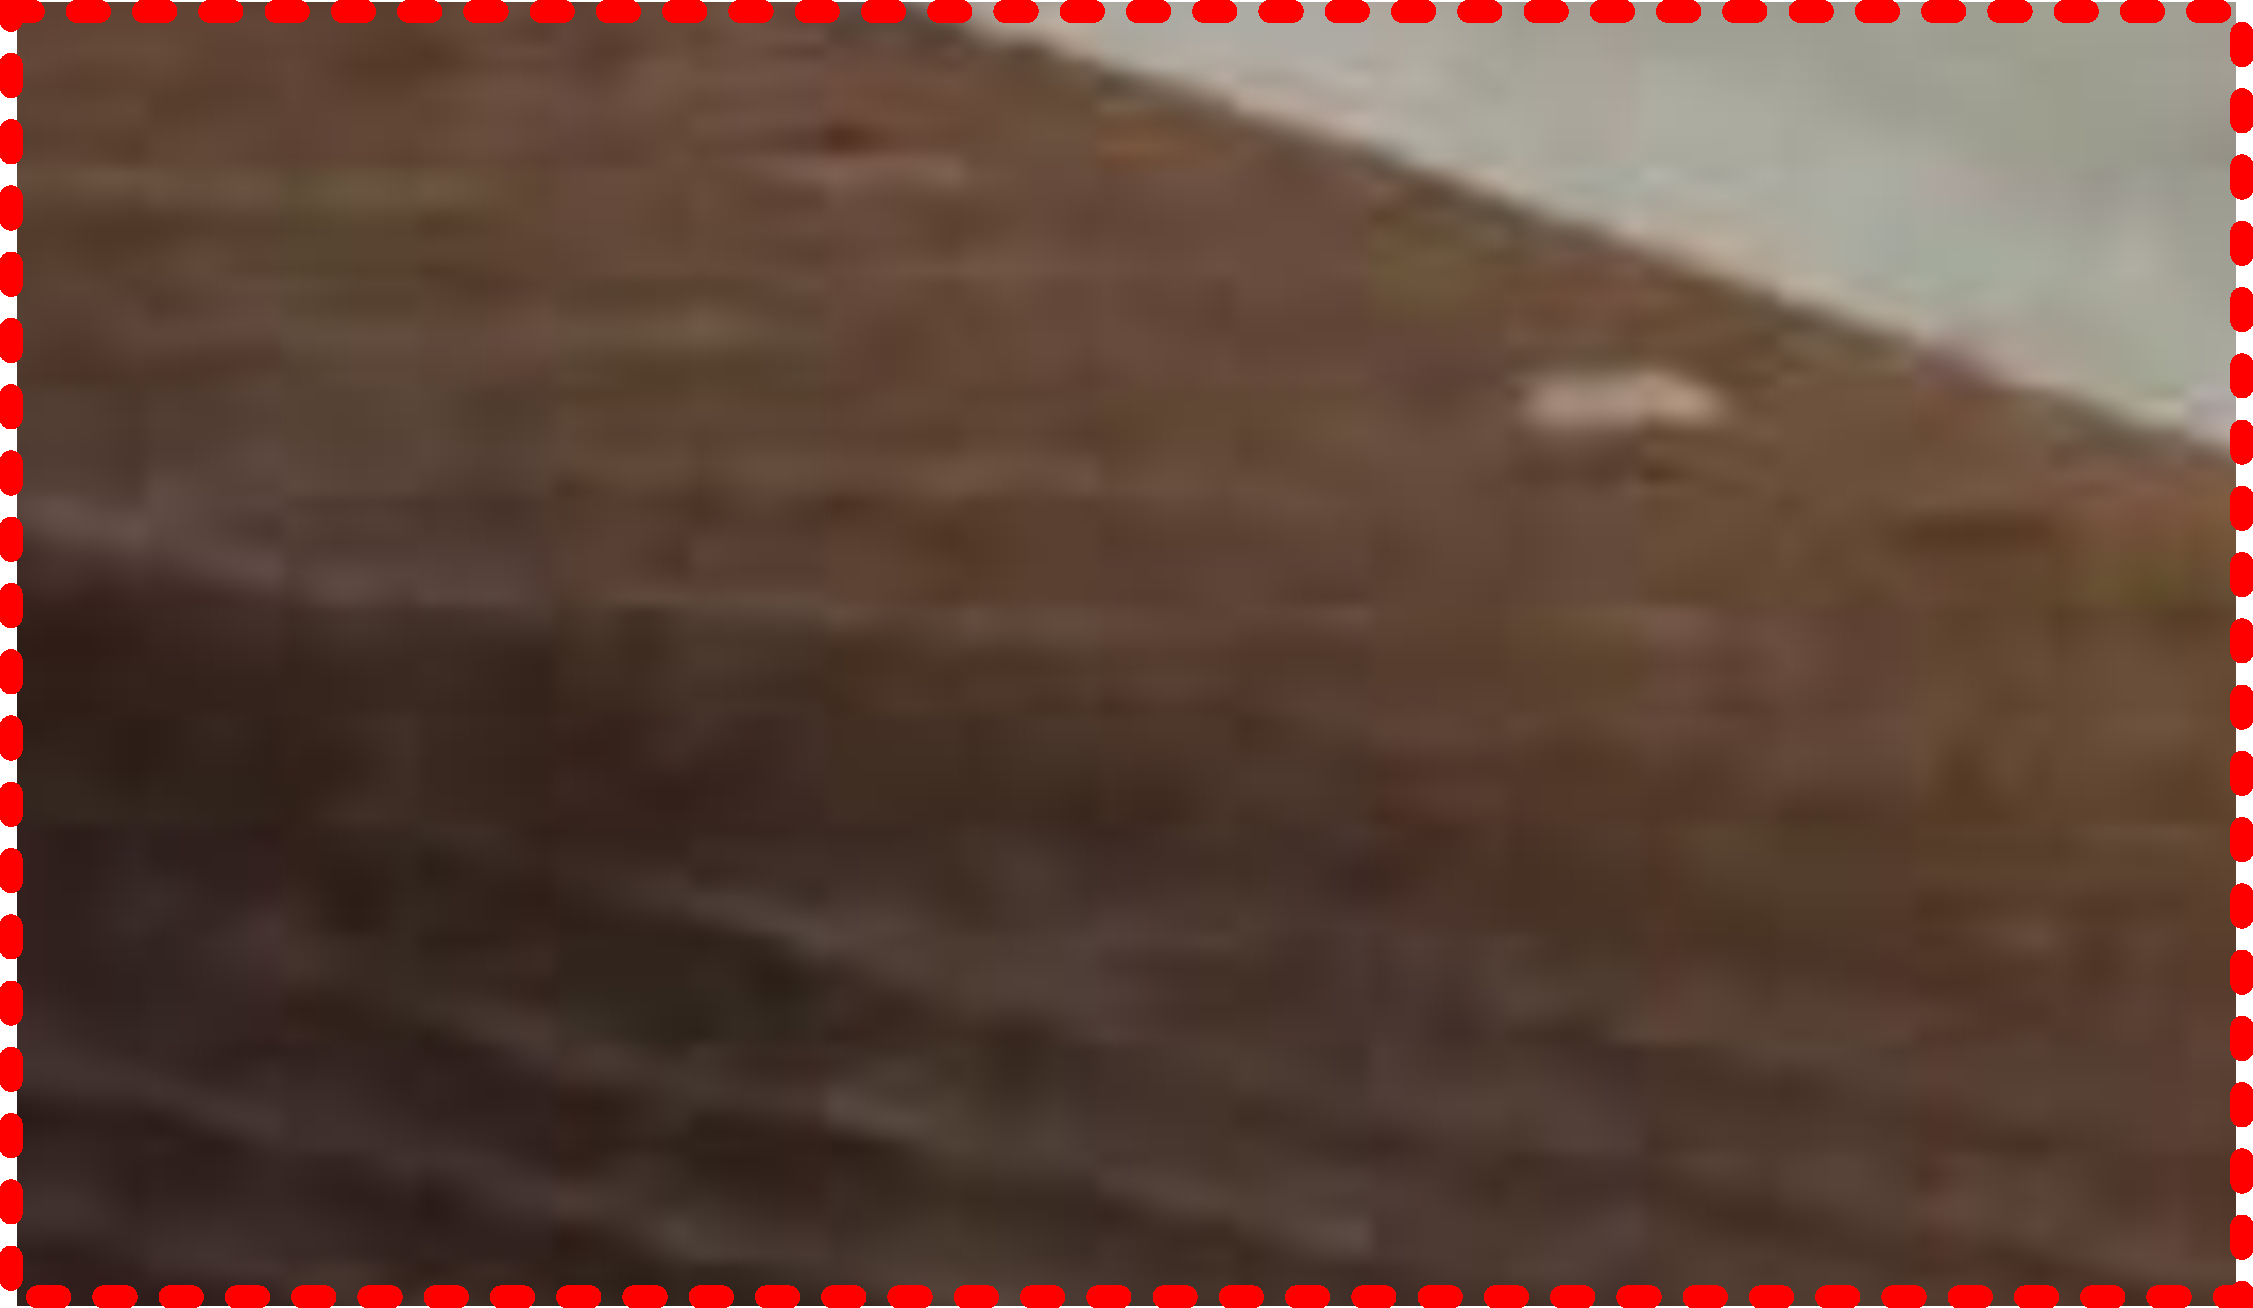
\includegraphics[width=4.5cm,height=3.5cm]{AAUgraphics/pt2/WingComparisonDirect}
	\end{multicols}
	

\end{frame}

\begin{frame}{Sistema de OCT a nivel del laboratorio}{Estructura ala de \emph{blattodea}: Sección transversal}
	\centering
	%\href{run:AAUmovies/Blattodea_BScan_with_line.avi}{
	%	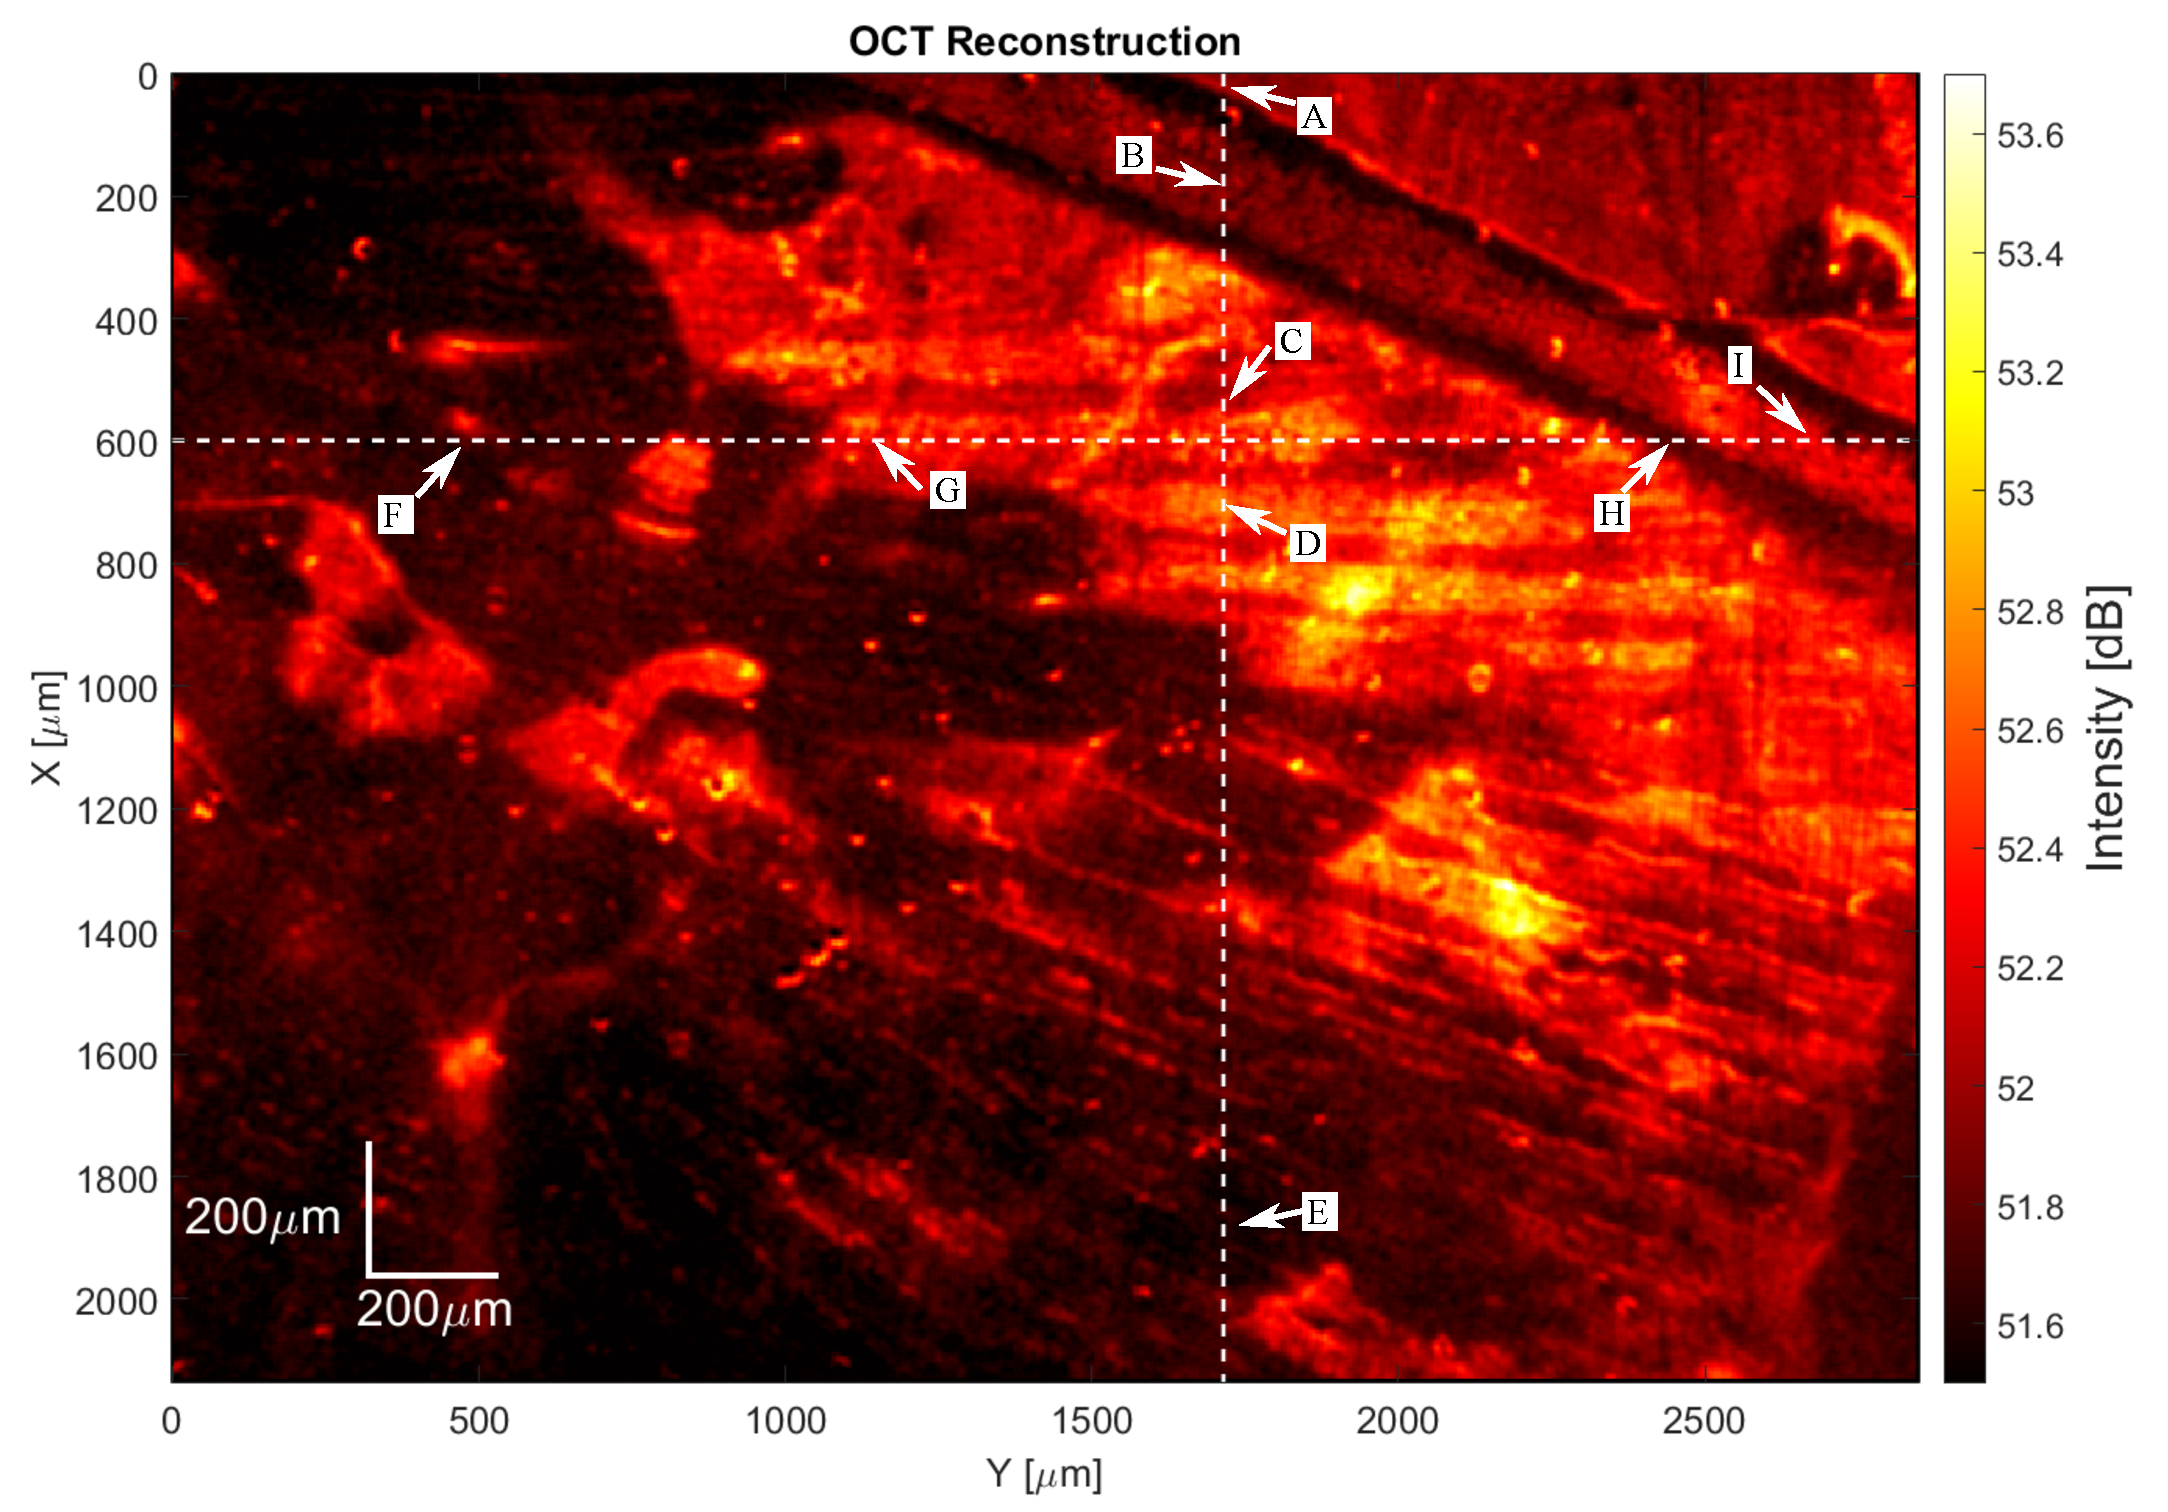
\includegraphics[width=0.49\linewidth]{AAUgraphics/pt2/OCT_projection_points}}
	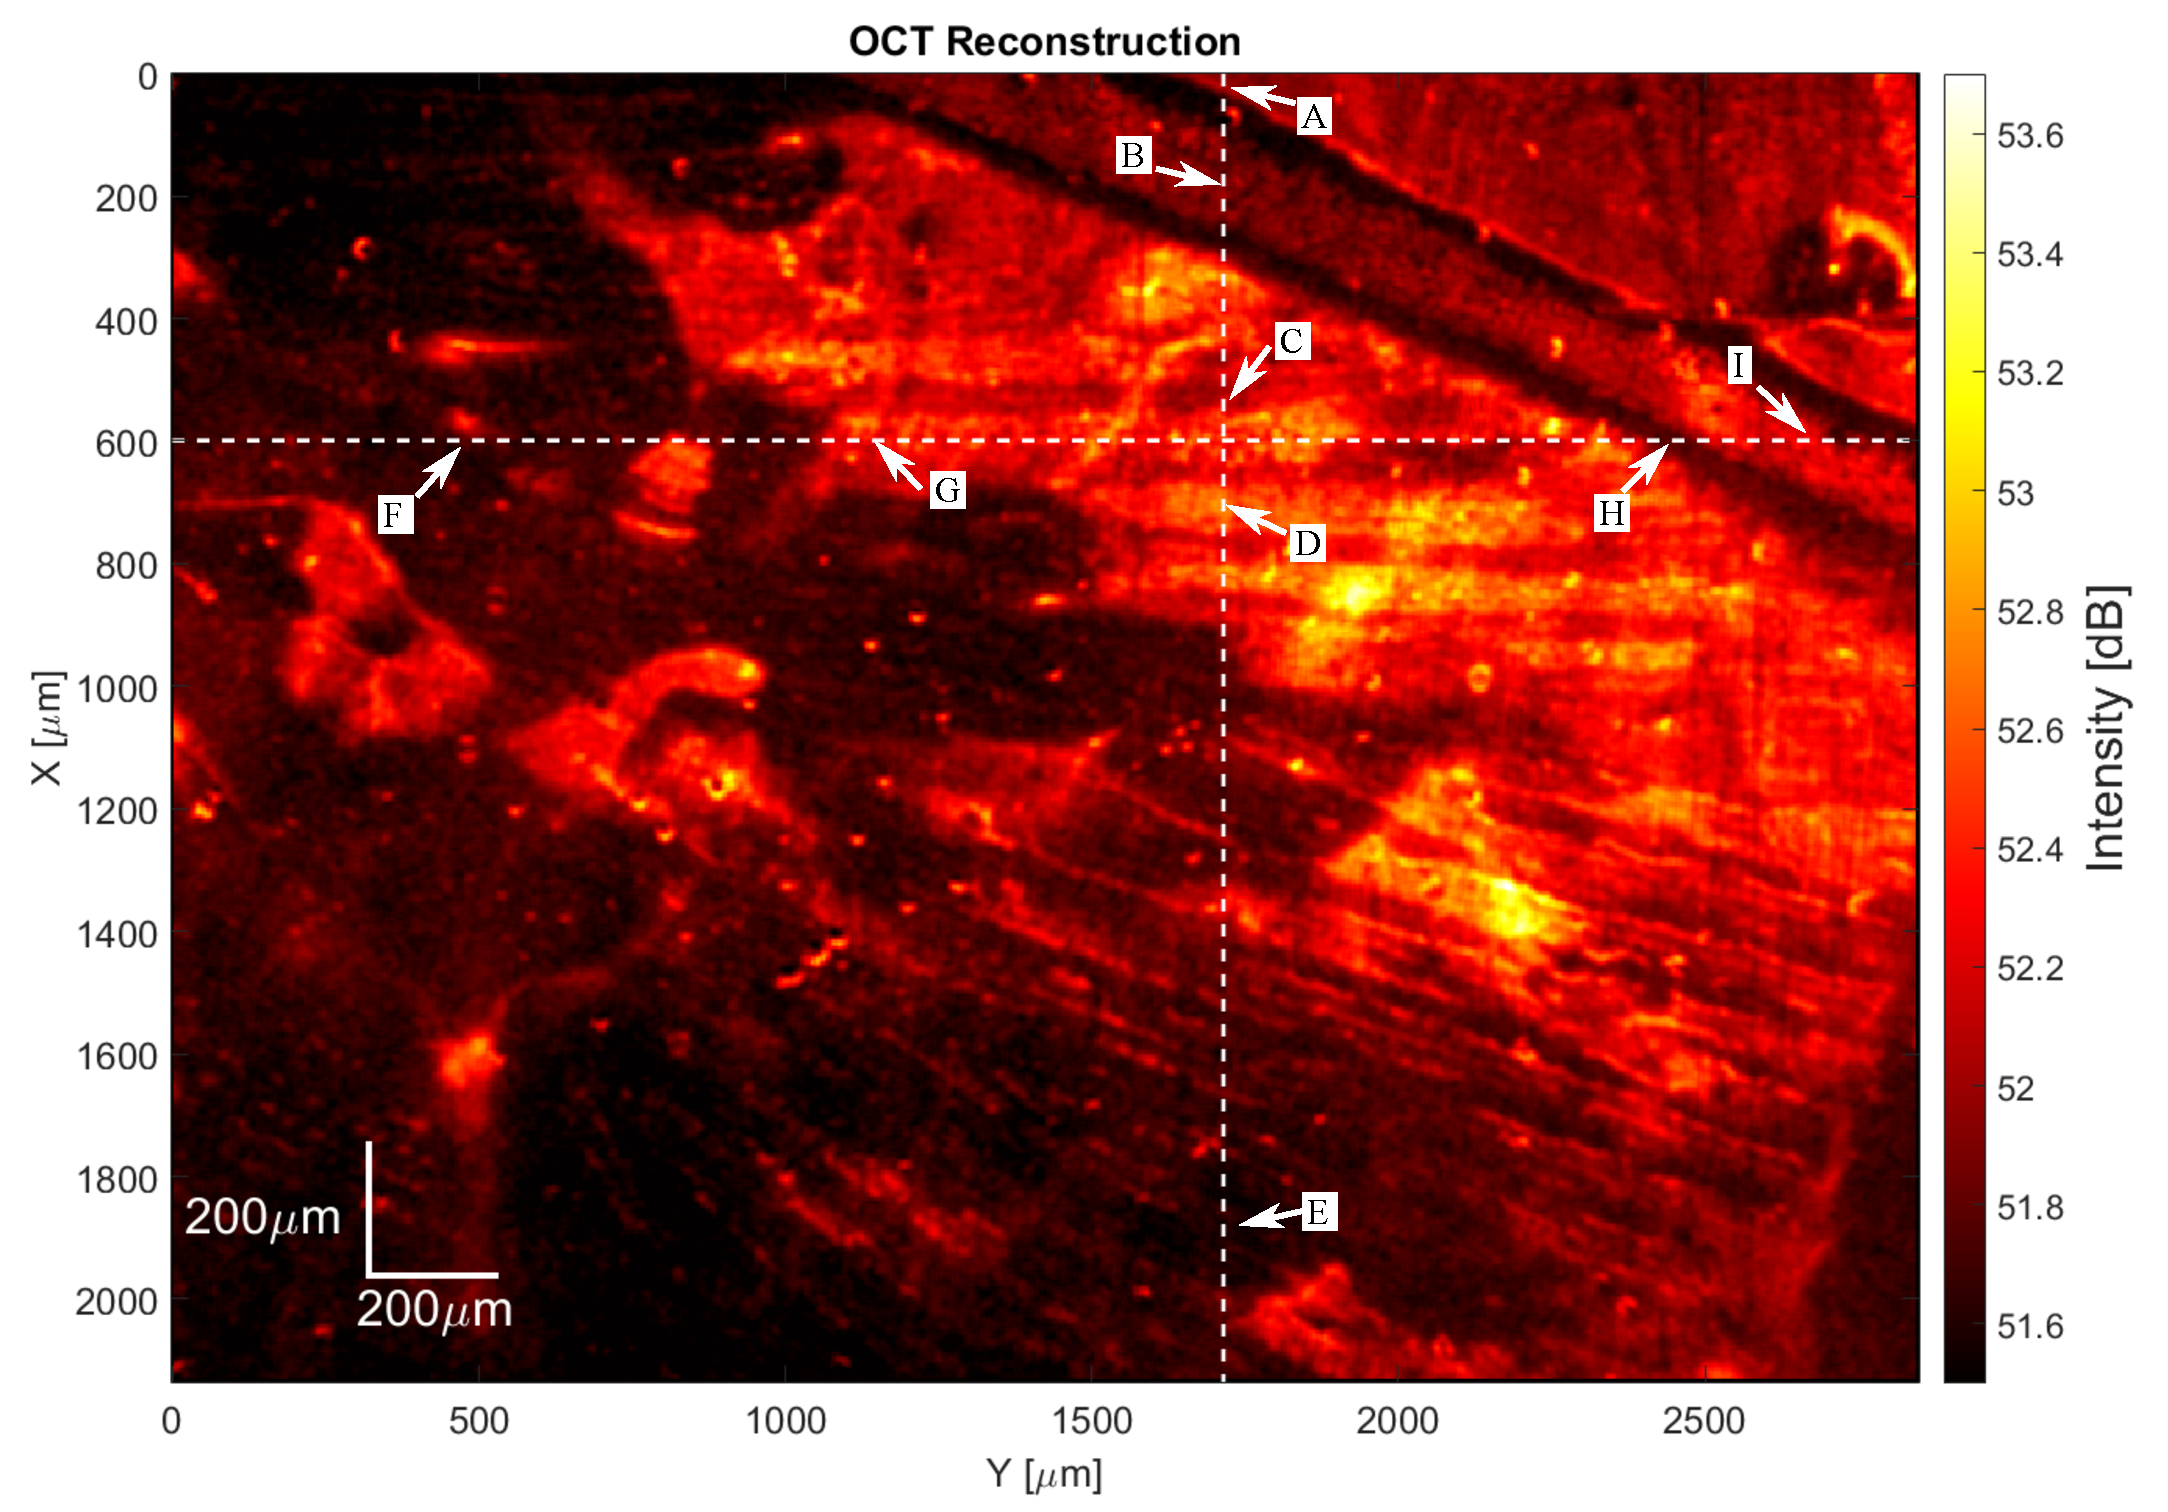
\includegraphics[width=0.6\linewidth]{AAUgraphics/pt2/OCT_projection_points}
	
	\vfill
	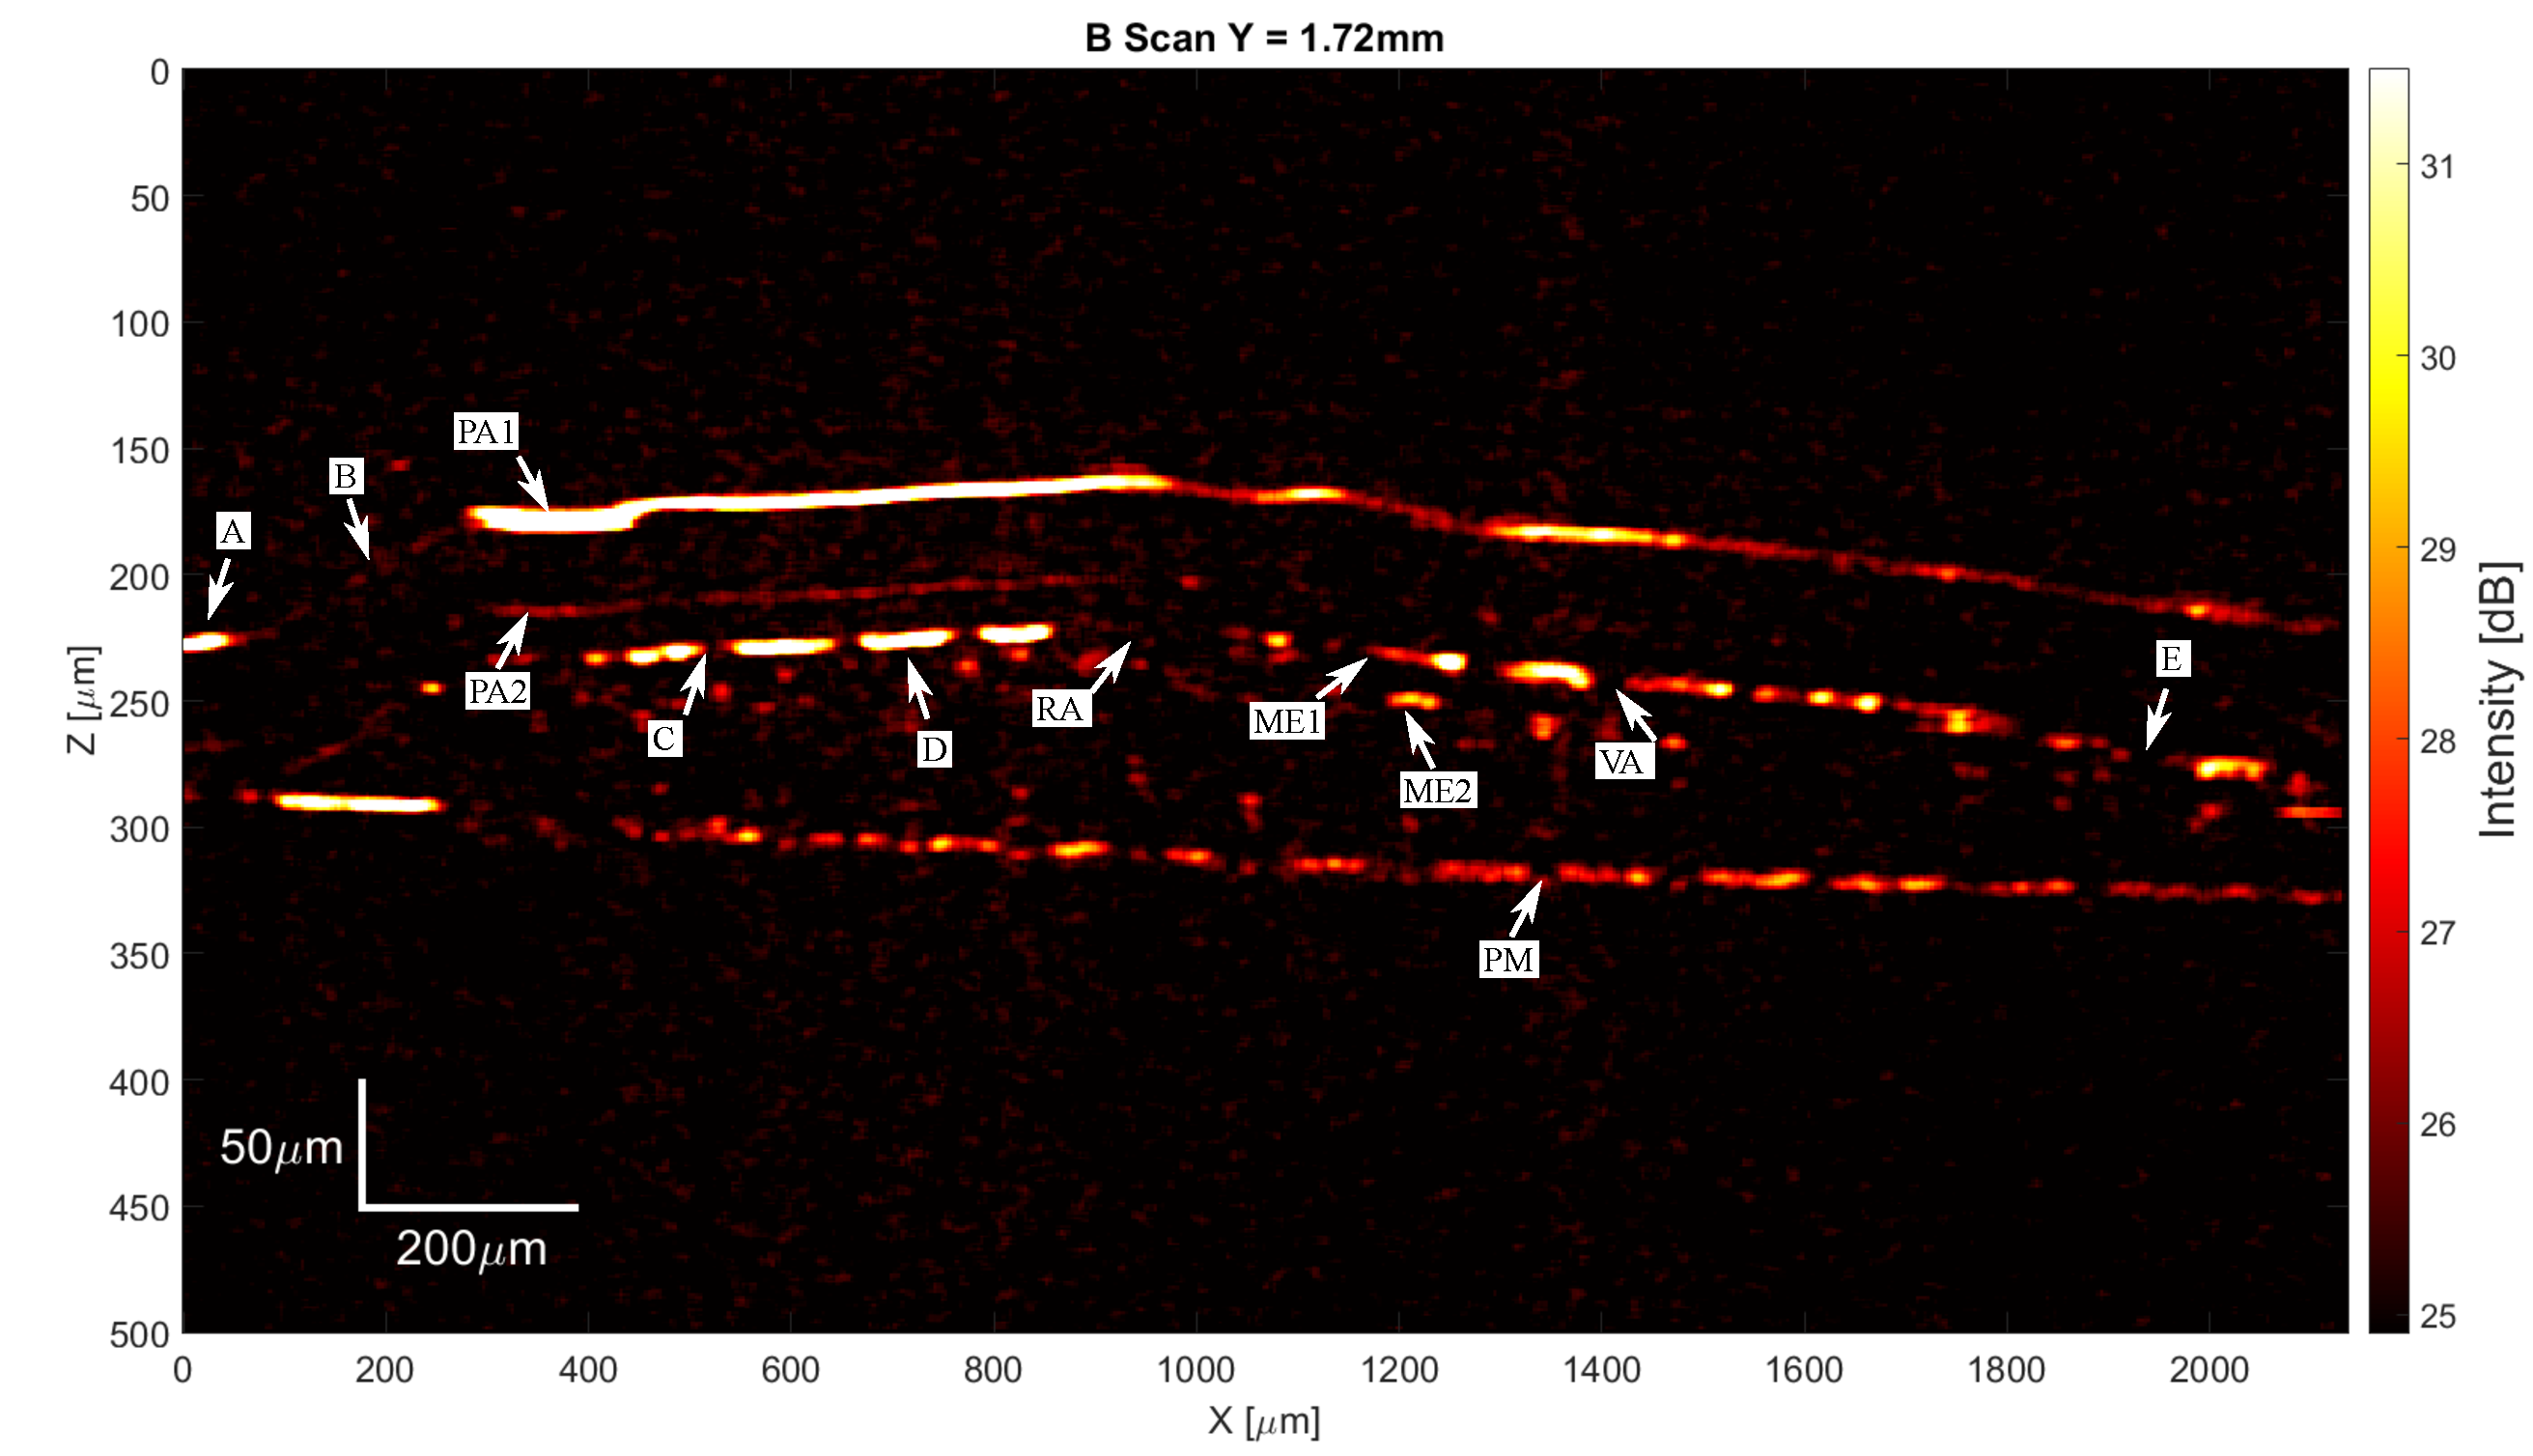
\includegraphics[width=0.49\linewidth]{AAUgraphics/pt2/Bscan_Wing}
	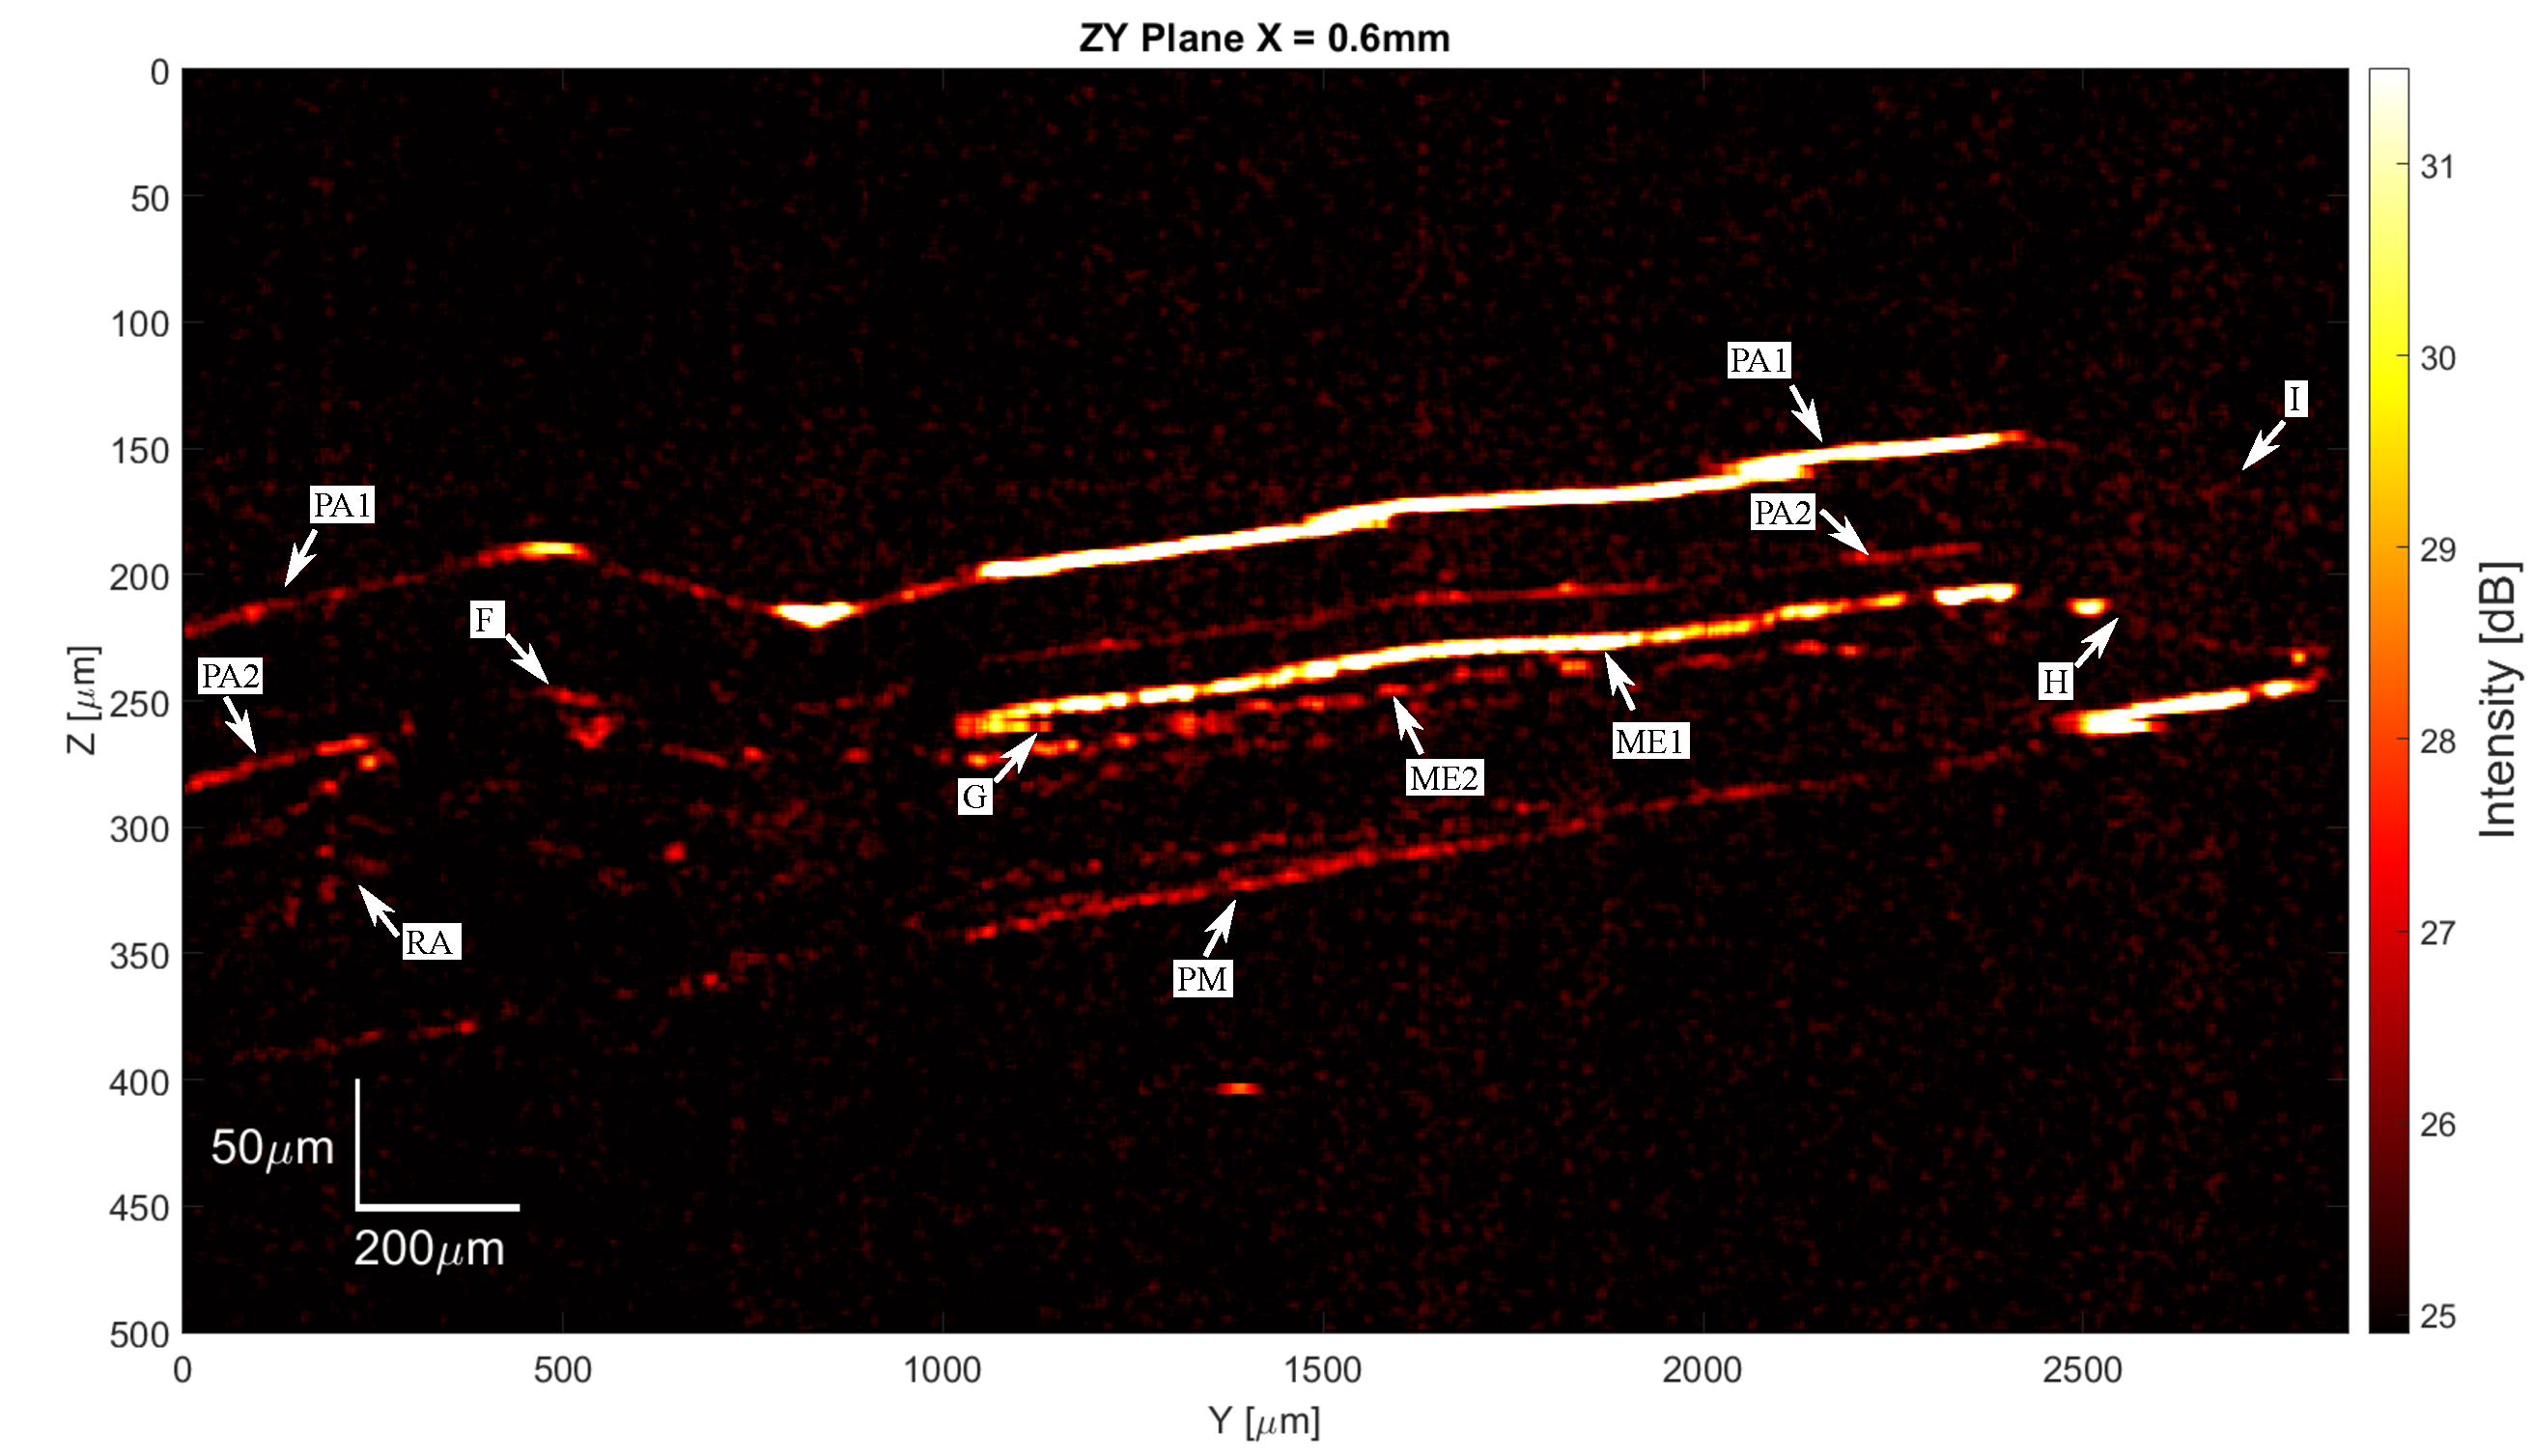
\includegraphics[width=0.49\linewidth]{AAUgraphics/pt2/ZY_Wing}
\end{frame}

\begin{frame}{Sistema de OCT a nivel del laboratorio}{Estructura ala de \emph{blattodea}: Sección transversal}
	\begin{center}
		%\addtocounter{framenumber}{-1}
		\movie[width = \linewidth, height= 0.55\linewidth, loop, autostart, poster] {}{AAUmovies/Blattodea_BScan_with_line.avi}
	\end{center}
\end{frame}

%\begin{frame}{Sistema de OCT a nivel del laboratorio}{Estructura ala de \emph{blattodea}: Renderizado}
%	%\href{run:AAUmovies/Battodea_3D_Slow_motion.avi}{
%	%	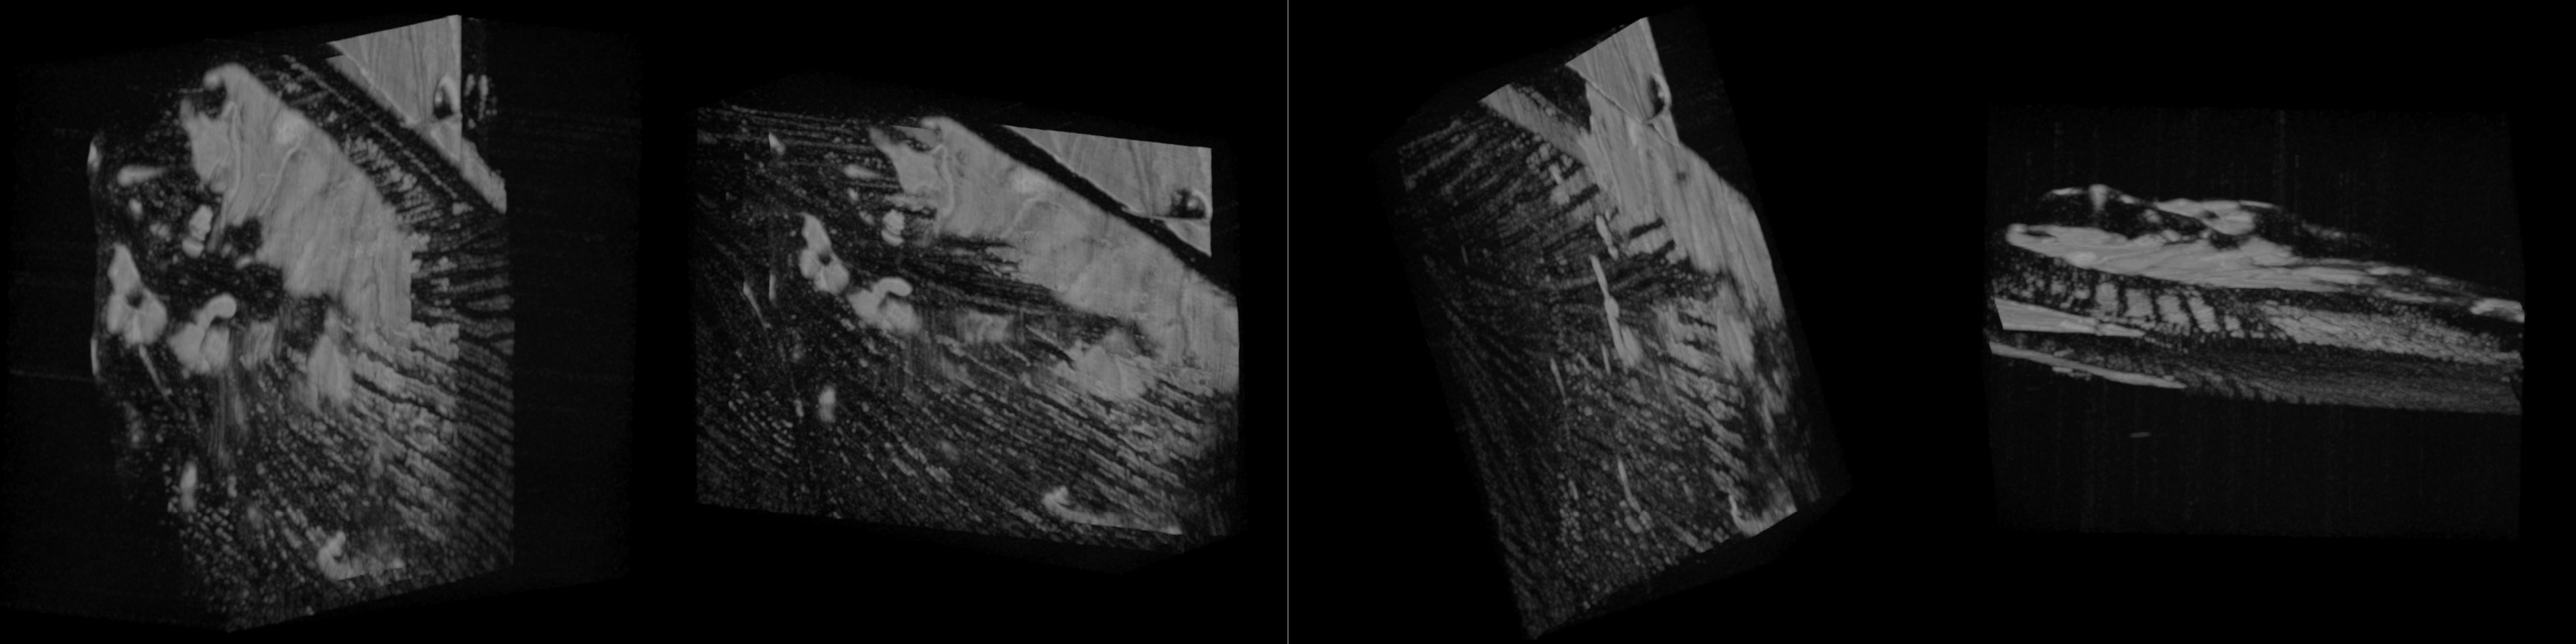
\includegraphics[width=1\linewidth]{AAUgraphics/pt2/Perspectivas_wing}}
%	
%	\begin{center}
%		\movie[width = \linewidth, height= 0.55\linewidth, loop, autostart, poster] {}{AAUmovies/Battodea_3D_Slow_motion.avi}
%	\end{center}
%	
%\end{frame}


%---------------------------------------------------------------%
\section{Supresión del ruido por \emph{speckle} en imágenes de OCT}
% Section frame
\begin{frame}{Contenido}
	%\addtocounter{framenumber}{-1}
	\tableofcontents[currentsection]
\end{frame}

%%%%%%%%%%%%%%%%%%%%%%%%%%
%\subsection{¿Qué es el speckle?}
\begin{frame}{¿Dónde aparece el \emph{speckle}?}
	Aparece en las técnicas de imagen coherente como MRI, USI, SAR y OCT.\blfootnote{\noindent\scalebox{.5}{ \url{http://opfocus.org/index.php?topic=picture&v=17&s=7&p=1}  \url{http://www.ee.nmt.edu/~erives/552_11/Ultrasound_SpeckleNoise.bmp}} \scalebox{0.5}{
			\url{https://www.intechopen.com/source/html/9501/media/image3.jpg}} \scalebox{0.5}{\url{http://www.jmp.org.in/articles/2016/41/4/images/JMedPhys_2016_41_4_254_195190_f3.jpg}} }
	\vfill
	
	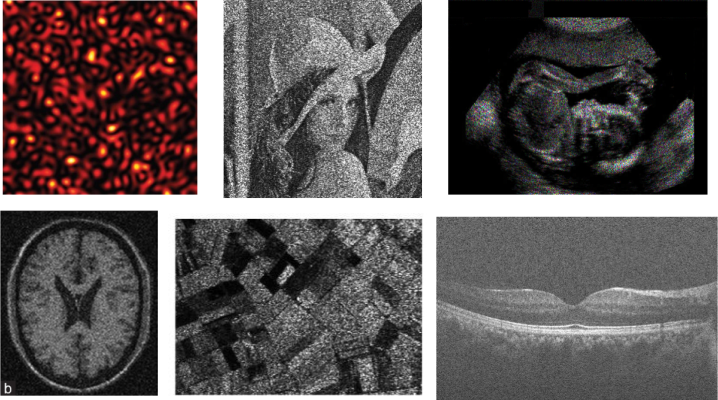
\includegraphics[width=0.95\linewidth]{AAUgraphics/pt3/speckle}
\end{frame}

%%%%%%%%%%%%%%%%%%%%%%%%%%
\subsection[Formación y características del \emph{speckle}]{Formación y características del \emph{speckle} en OCT}
\begin{frame}{Formación y características del \emph{speckle} en OCT}
	\vspace*{-0.5cm}
		\blfootnote{{\tiny M. Bashkansky and J. Reintjes. Statistics and reduction of speckle on optical coherence tomography. \emph{Opt. Lett.} \textbf{25}(8):545.547, 1999.}}
	\begin{multicols}{2}{\footnotesize 
		\noindent Señal interferométrica
		 \begin{equation*}
			i_D = \rho \langle\lvert E_R\rvert^2 + \lvert E_S \rvert^2 + 2E_R E_S \cos(2 k_0 \Delta z)\rangle.
			\end{equation*}
		
		\pause
		\noindent Función de densidad de probabilidad luz polarizada
		\begin{equation*}
			p(I) = \frac{1}{\bar{I}} \exp \left(- \frac{I}{\bar{I}}\right),
		\end{equation*}
		$SNR = 1$.\\
		\vspace*{0.5cm}
		
		\noindent Función de densidad de probabilidad luz no polarizada
		\begin{equation*}
			p(I) = \frac{4I}{\bar{I}^2} \exp \left(-2 \frac{I}{\bar{I}}\right),
		\end{equation*}
		$SNR = 1.4$.}
		
		\newpage
		
		\includegraphics[width=1\linewidth]{AAUgraphics/pt3/sample_backscattering}
		
	\end{multicols}
\end{frame}

%%%%%%%%%%%%%%%%%%%%%%%%%%
%\subsection{Del filtrado en SAR a OCT}
\begin{frame}{Del filtrado en SAR a OCT}{\emph{Non-Local Means}}
	%Filtrado de imágenes provenientes de Titan, una luna de Saturno, empleando \emph{Non-Local Means}.\blfootnote{{\tiny \url{http://dralucas.geophysx.org/res.html}}}\blfootnote{{\tiny A. Lucas \emph{et al.} Insights into Titan's geology and hydrology based on enhanced image processing of cassini radar data. \emph{Gephys. Res. Planets}, \textbf{119}:2149-2166, 2014.}}
	Filtrado de imágenes provenientes de Titan, una luna de Saturno, empleando \emph{Non-Local Means}.\blfootnote{{\tiny A. Lucas \emph{et al.} Insights into Titan's geology and hydrology based on enhanced image processing of cassini radar data. \emph{Gephys. Res. Planets}, \textbf{119}:2149-2166, 2014.}}
	\begin{center}
		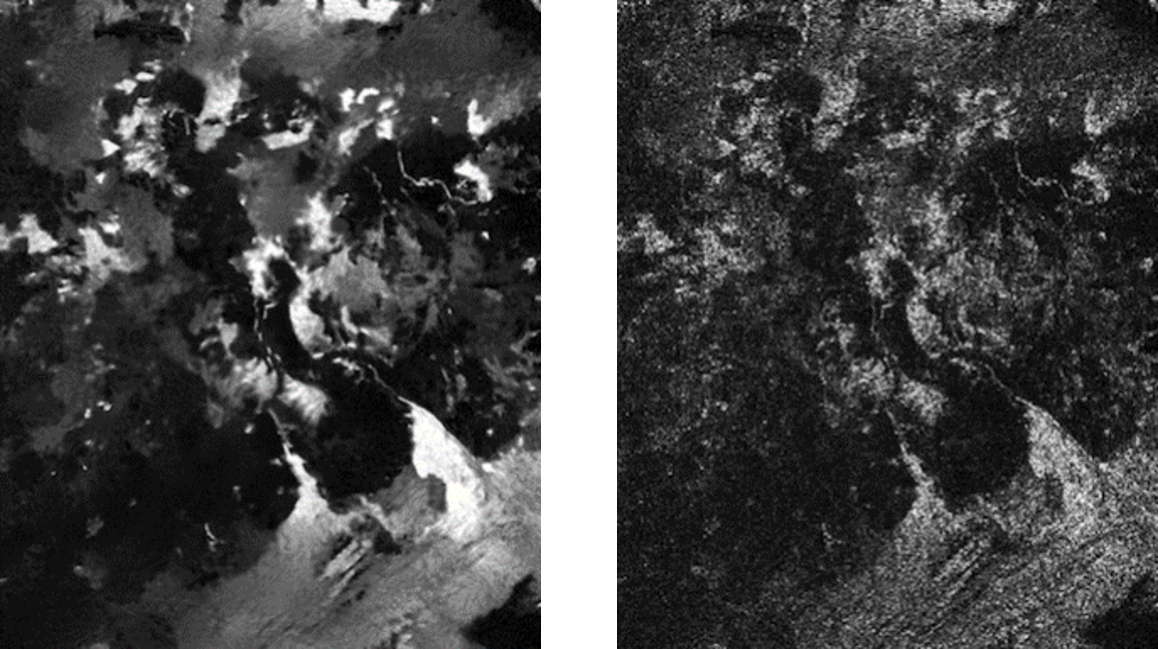
\includegraphics[width=0.9\linewidth]{AAUgraphics/pt3/Titan_speckle}
	\end{center}
	\hspace*{1cm}Imagen filtrada \hspace*{3cm} Imagen ruidosa
\end{frame}

%%%%%%%%%%%%%%%%%%%%%%%%%%
%\subsection{¿Qué es \emph{Non-local Means} (\emph{NL-Means})?}
\begin{frame}{¿Qué es \emph{Non-local Means} (\emph{NL-Means})?}{Concepto}
	\emph{NL-Means} emplea la redundancia existente en un imagen natural para realizar el filtrado, comparando pequeñas ventanas de la imagen.
	\begin{center}
		\includegraphics[width=0.6\linewidth]{AAUgraphics/pt3/lennaPatches}
	\end{center}
\end{frame}

%%%%%%%%%%%%%%%%%%%%%%%%%%
%\subsection{\emph{NL- Means} con PPB}
\begin{frame}{¿Qué es \emph{Non-local Means} (\emph{NL-Means})?}{Teoría}
	
\blfootnote{{\tiny 	A. Baudes \emph{et al.} \emph{Multiscale modeling and simulation,} \textbf{4}(2):490-530, 2005.}}  \blfootnote{{\tiny C. Deledalle \emph{et al.} \emph{IEEE Transaction in image processing,} \textbf{18}(12):2661-2672, 2009.}}

%\blfootnote{{\tiny 	A. Baudes \emph{et al.} A review of image denoising algorithms, with a new one. \emph{Multiscale modeling and simulation,} \textbf{4}(2):490-530, 2005.}}  \blfootnote{{\tiny C. Deledalle \emph{et al.} Iterative maximum likelihood denoising with probabilistic patch based weights. \emph{IEEE Transaction in image processing,} \textbf{18}(12):2661-2672, 2009.}}
	
	\vspace*{-1cm}
	\begin{multicols}{2}
		\vfill
		{\footnotesize En \emph{NL-Means} se comparan dos ventanas $\Delta_s$ y $\Delta_t$, conocidas como ventanas de similaridad, en una vecindad $\Psi_s$. El filtrado se regula con un criterio de similaridad entre estas ventanas. }
		\vfill
		\includegraphics[width=1\linewidth]{AAUgraphics/pt3/patches} 
		\newpage
		\pause
		
		{\footnotesize Estimador de pesos de máxima probabilidad:}
		{\scriptsize \begin{equation*}
			\hat{R}_s = \frac{\sum_t w(s,t) R_t}{\sum_t w(s,t)}.
			\end{equation*}}
		
		\pause
		{\footnotesize Pesos \emph{NL-Means} versión inicial:}
		{\scriptsize \begin{equation*}
			w(s,t) = \exp\left(-\frac{1}{h} \sum_k \alpha_k \lvert R_{s,k}-R_{t,k} \rvert^2 \right).
			\end{equation*}}
		
		\pause
		{\footnotesize Pesos \emph{NL-Means} con \emph{probabilistic patch based weights} (PPB):}
		{\scriptsize \begin{align*}
			\hspace*{-0.25cm}w(s,t) =&  \exp\Bigg( -\sum_{k}\Bigg[ \frac{1}{h} \log \left(\frac{A_{s,k}}{A_{t,k}} + \frac{A_{t,k}}{A_{s,k}}\right)\\
			& + \frac{1}{T} \frac{\big\lvert\hat{R}^{i-1}_{s,k} - \hat{R}^{i-1}_{t,k}\big\rvert^2}{\hat{R}^{i-1}_{s,k}\hat{R}^{i-1}_{t,k}} \Bigg]\Bigg).
			\end{align*}}
		
	\end{multicols}
\end{frame}

%%%%%%%%%%%%%%%%%%%%%%%%%%
%\subsection{Resultado NL- Means con PPB}
%\begin{frame}{Resultados}{Filtrado con \emph{NL-Means} con PPB}
%	Filtrado de una imagen de la retina de un volumen de $512\times512\times256$ datos, empleando \emph{NL- Means} con PPB.
%	\vfill
%	\includegraphics[width=0.45\linewidth]{AAUgraphics/pt3/Retinal_NoisyImage_Bscan128}
%	\hfil
%	\includegraphics[width=0.45\linewidth]{AAUgraphics/pt3/Retinal_NLMeansIterativo_Bscan128}
%	
%	\hfil Imagen ruidosa \hspace*{2.8cm}  Imagen filtrada 
%\end{frame}

%\begin{frame}{Resultados}{Filtrado con \emph{NL-Means} con PPB}
%	%\addtocounter{framenumber}{-1}
%	Filtrado de una imagen de la retina de un volumen de $512\times512\times256$ datos, empleando \emph{NL- Means} con PPB.
%	\vfill
%	\includegraphics[width=0.45\linewidth]{AAUgraphics/pt3/Retinal_NoisyImage_Bscan128}
%	\hfil
%	\includegraphics[width=0.45\linewidth]{AAUgraphics/pt3/Retinal_NLMeansIterativo_Bscan128}
%	
%	\hfil Imagen ruidosa \hspace*{2.8cm}  Imagen filtrada 
%	
%	\blfootnote{{\tiny H. Yu \emph{et al.} Probability-based non-local means filter for speckle noise suppresion in optical coherence tomography. \emph{Opt. Lett.}, \textbf{41}(5):994-997, 2016.}}
%\end{frame}


%%%%%%%%%%%%%%%%%%%%%%%%%%
\subsection{Propuesta de filtrado \emph{NL- Means-OCT}}
\begin{frame}{Propuesta de filtrado \emph{NL- Means-OCT}}{Modificaciones a \emph{NL- Means} con PPB}
	 \blfootnote{{\tiny C. Deledalle \emph{et al.} \emph{IEEE Transaction in image processing,} \textbf{18}(12):2661-2672, 2009.}}
	  \blfootnote{{\tiny K. Lu \emph{et al.} \emph{Hindawi Publishing Corporation}, \textbf{2012}(438617):1-7, 2011.}}
	  %\blfootnote{{\tiny J. Darbon \emph{et al.} \emph{IEEE International Symposium on Biomedical Imaging: From Nano to Macro,} \text{2008}:1331-1334, 2008.}}
	  \vspace*{-0.7cm}
	\begin{multicols}{2}
		\includegraphics[width=1\linewidth]{AAUgraphics/pt3/patches_propuesta} 
		\newpage
		\pause
		Pesos \emph{NL- Means-OCT}:
		{\scriptsize \begin{equation*}
			\hspace*{-0.25cm}w(s,t) = \exp \left[-\sum_{k} \frac{1}{h} \log \left(\frac{A_{s,k}}{A_{t,k}} + \frac{A_{t,k}}{A_{s,k}}\right) \right].
			\end{equation*}}
		{\scriptsize \begin{block}{Características}
			\begin{itemize}
				\item Completamente \emph{no local}.	
				\item Combinación conceptos 2D y 3D.
				\item Ventana de similaridad cúbica, debe conservar estructuras volumétricas.
				\item Requiere información volumétrica.
				\item Adaptado al ruido por \emph{speckle}, desde su estadística.
				\item Filtrado en múltiples direcciones.
				{\color{violet}	\item Tiempo de procesamiento comparable al \emph{NL-Means}.
					\item Ventanas ortotrópicas.}
%				\item<1-> Completamente \emph{no local}.	
%				\item<2-> Combinación conceptos 2 y 3D.
%				\item<3-> Ventana de similaridad cúbica, debe conservar estructuras volumétricas.
%				\item<4-> Requiere información volumétrica.
%				\item<5-> Adaptado al ruido por \emph{speckle}, desde su estadística.
%				\item<6-> Filtrado en múltiples direcciones.
			\end{itemize}
		\end{block}}
	\end{multicols}
\end{frame}

%%%%%%%%%%%%%%%%%%%%%%%%%%
\subsection[Resultados]{Resultados obtenidos y aplicaciones}
%\begin{frame}
%	Este es un frame dummy
%\end{frame}

%%%%%%%%%%%%%%%%%%%%%%%%%%
%\subsubsection{OCT en la retina}
%\begin{frame}{Resultados obtenidos y aplicaciones}{OCT en la retina: filtrado con NL-Means-OCT en ZX}
%	Comparación de las imágenes filtradas con \emph{NL-Means} con PPB y \emph{NL-Means-OCT}, para el volumen de $512\times512\times256$ datos. El tiempo de procesamiento fue de $69.3h$ $16min/img$ {\color{violet} ($2.11h$ $(22s/img)$)}, $W=21\times21$, $\Delta = 7\times7\times7$ y $h=18$. 
%	\blfootnote{{\tiny J. Darbon \emph{et al.} Fast nonlocal filtering applied to electron cryomiscroscopy. \emph{IEEE International Symposium on Biomedical Imaging: From Nano to Macro,} \text{2008}:1331-1334, 2008.}}
%	\vfill
%	
%	\begin{center}
%		\includegraphics[width=0.325\linewidth]{AAUgraphics/pt3/Retinal_NoisyImage_Bscan128}	
%		\hspace*{0.025cm}
%		\includegraphics[width=0.325\linewidth]{AAUgraphics/pt3/Retinal_NLMeansIterativo_Bscan128}
%		\href{run:AAUmovies/Retinal-IntVideo-CrossSections-ZX.avi}{
%			\includegraphics[width=0.325\linewidth]{AAUgraphics/pt3/Retinal/FinalResult_ZX}}
%	\end{center}
%	\vspace*{-0.3cm}
%	\hspace*{0.35cm} Imagen ruidosa \hspace*{0.55cm} \emph{NL-Means} con PPB \hspace*{0.4cm} \emph{NL-Means-OCT}
%\end{frame}

\begin{frame}{Resultados obtenidos y aplicaciones}{OCT en la retina: filtrado con NL-Means-OCT en ZX}
	Comparación de las imágenes filtradas con \emph{NL-Means} con PPB y \emph{NL-Means-OCT}, para el volumen de $512\times512\times256$ datos. El tiempo de procesamiento fue de $69.3h$ $(16min/img)$ {\color{violet} [$2.11h$ $(22s/img)$]}, $W=21\times21$, $\Delta = 7\times7\times7$ y $h=18$. 
	%\blfootnote{{\tiny J. Darbon \emph{et al.} Fast nonlocal filtering applied to electron cryomiscroscopy. \emph{IEEE International Symposium on Biomedical Imaging: From Nano to Macro,} \text{2008}:1331-1334, 2008.}}
	\vfill
	
%	\begin{tikzpicture}[remember picture,overlay]
%	\node[xshift=-0.0cm,yshift=0cm] at (current page.south east)
%	{\movie[width = \linewidth, showcontrols,once] {play}{AAUmovies/Retinal-IntVideo-CrossSections-ZX.avi}};
%	\end{tikzpicture}
	
%	\begin{center}
%		\movie[width = \linewidth, showcontrols,once,height=5cm] {\includegraphics[width=0.325\linewidth]{AAUgraphics/pt3/Retinal_NoisyImage_Bscan128}}{AAUmovies/Retinal-IntVideo-CrossSections-ZX.avi}
%		%\includegraphics[width=0.325\linewidth]{AAUgraphics/pt3/Retinal_NoisyImage_Bscan128}
%		\hspace*{0.03cm}
%		\includegraphics[width=0.325\linewidth]{AAUgraphics/pt3/Retinal_NLMeansIterativo_Bscan128}
%		%\includegraphics[width=0.325\linewidth]{AAUgraphics/pt3/Retinal/FinalResult_ZX}
%		\href{run:AAUmovies/Retinal-IntVideo-CrossSections-ZX.avi}{
%		\includegraphics[width=0.325\linewidth]{AAUgraphics/pt3/Retinal/FinalResult_ZX}}
%	\end{center}
	
		\begin{center}
			\includegraphics[width=0.325\linewidth]{AAUgraphics/pt3/Retinal_NoisyImage_Bscan128}
			%\includegraphics[width=0.325\linewidth]{AAUgraphics/pt3/Retinal_NoisyImage_Bscan128}
			\hfill
			\includegraphics[width=0.325\linewidth]{AAUgraphics/pt3/Retinal_NLMeansIterativo_Bscan128}
			%\includegraphics[width=0.325\linewidth]{AAUgraphics/pt3/Retinal/FinalResult_ZX}
			\hfill
			\includegraphics[width=0.325\linewidth]{AAUgraphics/pt3/Retinal/FinalResult_ZX}
		\end{center}
	\vspace*{-0.3cm}
	\hspace*{0.35cm} Imagen ruidosa \hspace*{0.55cm} \emph{NL-Means} con PPB \hspace*{0.4cm} \emph{NL-Means-OCT}
\end{frame}

\begin{frame}{Resultados obtenidos y aplicaciones}{OCT en la retina: filtrado con NL-Means-OCT en ZX}
	%\addtocounter{framenumber}{-1}
	\vspace*{-0.2cm}
	\begin{center}
		\movie[width = 0.45\linewidth, height= 0.8\linewidth, loop, autostart] {}{AAUmovies/Retinal-IntVideo-CrossSections-ZX.avi}
	\end{center}
\end{frame}

\begin{frame}{Resultados obtenidos y aplicaciones}{OCT en la retina: filtrado con NL-Means-OCT en ZX y ZY.}
	No se encontraron diferencias significativas si el plano de la ventana de búsqueda es el mismo.
	\vfill
	
	\includegraphics[width=0.325\linewidth]{AAUgraphics/pt3/Retinal_NoisyImage_Bscan128}
	\hfill
	\includegraphics[width=0.325\linewidth]{AAUgraphics/pt3/Retinal/FinalResult_ZX}
	\hfill
	\includegraphics[width=0.325\linewidth]{AAUgraphics/pt3/Retinal/FinalResult_ZY}
	
%		\includegraphics[width=0.325\linewidth]{AAUgraphics/pt3/Retinal_NoisyImage_Bscan128}
%		\href{run:AAUmovies/Retinal-IntVideo-CrossSections-ZX-MotionCorrected.avi}{
%			\includegraphics[width=0.325\linewidth]{AAUgraphics/pt3/Retinal/FinalResult_ZX}}
%		\includegraphics[width=0.325\linewidth]{AAUgraphics/pt3/Retinal/FinalResult_ZY}
%		
	\hspace*{0.5cm} Imagen ruidosa \hspace*{0.7cm} Filtrado en $ZX$ \hspace*{0.7cm} Filtrado en $ZY$ 
\end{frame}

%\begin{frame}{Resultados obtenidos y aplicaciones}{OCT en la retina: filtrado con NL-Means-OCT en ZX y ZY.}
%	\addtocounter{framenumber}{-1}
%	\vspace*{-0.2cm}
%	\begin{center}
%		\movie[width = 0.45\linewidth, height= 0.8\linewidth, loop, autostart] {}{AAUmovies/Retinal-IntVideo-CrossSections-ZX-MotionCorrected.avi}	
%	\end{center}
%\end{frame}

\begin{frame}{Resultados obtenidos y aplicaciones}{OCT en la retina: Proyecciones \emph{en-face}.}
	Comparación de las proyecciones \emph{en-face} luego del filtrado. Se aprecia la aparición de \emph{líneas} en la dirección sobre la cual se encuentra ubicada la ventana de búsqueda.
	\vfill
	
	\includegraphics[width=0.22\linewidth]{AAUgraphics/pt3/Retinal/EnfaceNoisy}
	\hfill
	\includegraphics[width=0.22\linewidth]{AAUgraphics/pt3/Retinal/EnfaceZX}
	\hfill
	\includegraphics[width=0.22\linewidth]{AAUgraphics/pt3/Retinal/EnfaceZY}
	\hfill
	\includegraphics[width=0.22\linewidth]{AAUgraphics/pt3/Retinal/Enface3D}
	\hspace*{0.025cm}
	
%		\href{run:AAUmovies/Retinal-IntVideo-Enface-ZXFilt-2.avi}{
%			\includegraphics[width=0.22\linewidth]{AAUgraphics/pt3/Retinal/EnfaceNoisy}}
%		\href{run:AAUmovies/Retinal-IntVideo-MotionCorrectedZX-2.avi}{
%			\includegraphics[width=0.22\linewidth]{AAUgraphics/pt3/Retinal/EnfaceZX}}
%		\href{run:AAUmovies/Retinal-IntVideo-Enface-MotionCorrectedZYFilt-2.avi}{
%			\includegraphics[width=0.22\linewidth]{AAUgraphics/pt3/Retinal/EnfaceZY}}
%		\hspace*{0.025cm}
%		\includegraphics[width=0.22\linewidth]{AAUgraphics/pt3/Retinal/Enface3D}
	
	\hspace*{0.5cm} Ruidosa \hspace*{0.7cm} Filtrado $ZX$ \hspace*{0.5cm} Filtrado $ZY$ \hspace*{0.6cm} Filtrado 3D 
\end{frame}

\begin{frame}{Resultados obtenidos y aplicaciones}{OCT en la retina: Proyecciones \emph{en-face}.}
		%\addtocounter{framenumber}{-1}
		\vspace*{-0.2cm}
		\begin{center}
			\movie[width = 0.85\linewidth, height= 0.8\linewidth, loop, autostart] {}{AAUmovies/Retinal-IntVideo-MotionCorrectedZX-2.avi}	
		\end{center}
\end{frame}

%%%%%%%%%%%%%%%%%%%%%%%%%%
%\subsubsection{OCT en tractografía}
%\begin{frame}{Resultados obtenidos y aplicaciones}{OCT en tractografía: CLARITY}
%	Proceso de \emph{blanqueado} para tejidos como el cerebro, permite el análisis con técnicas ópticas como la microscopía.
%	\vfill
%	
%	\centering
%	\includegraphics[width=0.8\linewidth]{AAUgraphics/pt3/Clarity_1}
%\end{frame}

\begin{frame}{Resultados obtenidos y aplicaciones}{OCT en tractografía: \emph{blanqueado} y expansión lineal (MAP)}
	Proceso de \emph{blanqueado} y expansión lineal de tejidos tales el cerebro. 
	\blfootnote{{\tiny T. Ku \emph{et al.} Multiplexed and scalable super-resolution imaging of three-dimensional protein localization in size-adjustable tissues. \emph{Nature}, \textbf{34}:973-981, 2016.}}
	\vfill
	
	\centering
	\includegraphics[width=0.9\linewidth]{AAUgraphics/pt3/Clarity_2}
\end{frame}

\begin{frame}{Resultados obtenidos y aplicaciones}{OCT en tractografía: Imágenes}
	El \emph{connectome} se realiza a partir de las sinapsis (puntos brillantes) que se presenta en las imágenes. 
	
	\vfill
	
	\centering
	Sección transversal:
	\includegraphics[width=1\linewidth]{AAUgraphics/pt3/Brain/ima_nsy_brain}
	
	\vfill
	
	Proyección \emph{en-face}:
	\includegraphics[width=1\linewidth]{AAUgraphics/pt3/Brain/Enface_nsy_brain}
	
	\vfill
	\raggedright
	Se tiene un volumen de  $160\times3600\times150$ con datos provenientes del cerebro de un ratón.
	
\end{frame}

\begin{frame}{Resultados obtenidos y aplicaciones}{OCT en tractografía: Resultados sección transversal}
	Imágenes de la sección transversal de las sinapsis. El tiempo de procesamiento fue de $35.4h$, $(14.1min/img)$ {\color{violet} [$2.5h, (1min/img)$]}, $W = 17\times17$, $\Delta = 7\times 7\times 7$ y $h=13$.
	
	\begin{multicols}{2}
		\centering
		Imagen ruidosa
		\includegraphics[width=1\linewidth]{AAUgraphics/pt3/Brain/ima_nsy_short_brain_lines}	
		\newpage
		Imagen filtrada
		\includegraphics[width=1\linewidth]{AAUgraphics/pt3/Brain/ima_filt_short_brain_lines}
	\end{multicols}
	\centering
	Imagen ruidosa
	\includegraphics[width=1\linewidth]{AAUgraphics/pt3/Brain/ima_nsy_brain_lines}
	%\href{run:AAUmovies/Tractography-IntVideo-CrossSections.avi}{
	%	\includegraphics[width=1\linewidth]{AAUgraphics/pt3/Brain/ima_filt_brain_lines}}
	
	Imagen filtrada
	\includegraphics[width=1\linewidth]{AAUgraphics/pt3/Brain/ima_filt_brain_lines}
\end{frame}

\begin{frame}{Resultados obtenidos y aplicaciones}{OCT en tractografía: Resultados proyección \emph{en-face}}
	Proyecciones \emph{en-face} con las imágenes de las sinapsis filtradas.
	
	\begin{multicols}{2}
		\centering
		Imagen ruidosa
		\includegraphics[width=1\linewidth]{AAUgraphics/pt3/Brain/Enface_zoomed_nsy_lines}
		\newpage
		Imagen filtrada
		\includegraphics[width=1\linewidth]{AAUgraphics/pt3/Brain/Enface_zoomed_filt_lines}
	\end{multicols}
	\centering
	Imagen ruidosa
	\includegraphics[width=1\linewidth]{AAUgraphics/pt3/Brain/Enface_nsy_brain_lines}
	%\href{run:AAUmovies/Tractography-IntVideo-Enface.avi}{
	%	\includegraphics[width=1\linewidth]{AAUgraphics/pt3/Brain/Enface_filt_brain_lines}}
	
	Imagen filtrada
	\includegraphics[width=1\linewidth]{AAUgraphics/pt3/Brain/Enface_filt_brain_lines}
\end{frame}

\begin{frame}{Resultados obtenidos y aplicaciones}{OCT en tractografía: Resultados proyección \emph{en-face}}
	%\addtocounter{framenumber}{-1}
	\vspace*{-0.2cm}
	\begin{center}
		\movie[width = \linewidth, height= 0.27\linewidth, loop, autostart] {}{AAUmovies/Tractography-IntVideo-Enface.avi}	
	\end{center}
\end{frame}


%%%%%%%%%%%%%%%%%%%%%%%%%%
%\subsubsection{OCT en gastroenterología}
\begin{frame}{Resultados obtenidos y aplicaciones}{OCT en gastroenterología}
%	En gastroenterología, el movimiento ocasionado por el paciente y el sistema de escaneo, además de la resolución en las tres direcciones dificulta el filtrado.
%		
	\blfootnote{{\tiny W. Drexler and J. Fujimoto. Optical coherence tomography: Technology and applications. Springer,  2015.}}
	\vfill
	\centering
	%\href{run:AAUmovies/GI-IntVideo-Polar-2.avi}{
	%	\includegraphics[width=0.9\linewidth]{AAUgraphics/pt3/GI}}
	\includegraphics[width=0.9\linewidth]{AAUgraphics/pt3/GI}
	
	\begin{tikzpicture}[remember picture,overlay]
	\node[xshift=-5.5cm,yshift=2.2cm] at (current page.south east) {%
		\movie[width = 3cm, height= 3cm, loop, poster] {}{AAUmovies/GI-IntVideo-Polar-2.avi}
	};
	\end{tikzpicture}	
			
%	\includemedia[
%	width=0.4\linewidth,
%	height=0.3\linewidth,
%	activate=pageopen,
%	passcontext,
%	addresource=AAUmovies/GI-IntVideo-CrossSections.mp4,
%	flashvars={source=AAUmovies/GI-IntVideo-CrossSections.mp4}
%	]{\fbox{asdfa}}{VPlayer.swf}

%	\begin{tikzpicture}[remember picture,overlay]
%	\node[anchor=south west, inner sep=0pt] at (current page.south west) {%
%		\movie[height = \paperheight, width = \paperwidth, poster, showcontrols] {}{AAUmovies/GI-IntVideo-CrossSections.mp4}%
%	};
%	\end{tikzpicture}
%\movie[height = 5cm, width = 5cm] {}{AAUmovies/Coin_ZY_plane_with_line.avi}

\end{frame}

\begin{frame}{Resultados obtenidos y aplicaciones}{OCT en gastroenterología: Resultados}
	Se filtró un volumen de $732\times4096\times128$, con un tiempo de procesamiento de $124.7h$ $(58.45min/img)$ {\color{violet}[$12.6h$ ($5.9min/img$)]}, $W=13\times17$, $\Delta = 7\times 9 \times 5$ y $h=13$.
	\vfill
	
	\centering
	\includegraphics[width=0.45\linewidth]{AAUgraphics/pt3/GI/ima_nsy_short_GI_lines}
	%\href{run:AAUmovies/GI-IntVideo-Polar-FiltZX-2.avi}{
	%	\includegraphics[width=0.45\linewidth]{AAUgraphics/pt3/GI/ima_filt_short_GI_liens}}
	\includegraphics[width=0.45\linewidth]{AAUgraphics/pt3/GI/ima_filt_short_GI_liens}
	\vfill
	
	\includegraphics[width=1\linewidth]{AAUgraphics/pt3/GI/ima_nsy_GI_lines}
	
	\includegraphics[width=1\linewidth]{AAUgraphics/pt3/GI/ima_filt_GI_lines}
%	\href{run:AAUmovies/GI-IntVideo-CrossSections.mp4}{
%		\includegraphics[width=1\linewidth]{AAUgraphics/pt3/GI/ima_filt_GI_lines}}
\end{frame}

\begin{frame}{Resultados obtenidos y aplicaciones}{OCT en gastroenterología: Resultados}
	\addtocounter{framenumber}{-1}
	\vspace*{-0.2cm}
	\begin{center}
		\movie[width = \linewidth, height= 0.4\linewidth, loop, autostart] {}{AAUmovies/GI-IntVideo-CrossSections.mp4}	
	\end{center}
\end{frame}

%---------------------------------------------------------------%
\section{Estabilización de la fase en OCT}
% Section frame
\begin{frame}{Contenido}
	\addtocounter{framenumber}{-1}
	\tableofcontents[currentsection]
\end{frame}

%%%%%%%%%%%%%%%%%%%%%%%%%%
\subsection{OCT con fuente de barrido (OFDI)}
\begin{frame}{OCT con fuente de barrido (OFDI)}{Fundamentos}
%/media/rrestrepo/PEPINO/CAC_thesis/Presentacion_TrabajoGrado_CCuartas/AAUgraphics/pt4/gif
%\transduration<0-16>{0}
%\multiinclude[<+->][format=png, graphics={width=0.5\textwidth},start=0, end=16]{AAUgraphics/pt4/gif/pt}
%\animategraphics[loop,controls,width=\linewidth]{12}{something-}{0}{16}
%\animategraphics[loop,controls,width=\linewidth]{12}{AAUgraphics/pt4/gif/pt-}{1}{5}
	\vspace*{-1.0cm}
	\begin{equation*}
		i_D = \rho \langle\lvert E_R\rvert^2 + \lvert E_S \rvert^2 + 2E_R E_S \cos(2\overwrite[blue]{k_0}{$\lambda$} \Delta z)\rangle
	\end{equation*}
	\pause
	\centering
	%\vspace*{-0.5cm}
	%\animategraphics[loop,controls,width=0.5\linewidth]{10}{AAUgraphics/pt4/gif/pt-}{5}{27}	
		\movie[width = 0.5\linewidth,loop] {\includegraphics[width=0.5\linewidth]{AAUgraphics/pt4/gif/pt-0.png}
		}{AAUgraphics/pt4/gif/out.mp4}
	\vfill
	%\pause
	\includegraphics[width=0.6\linewidth]{AAUgraphics/pt4/SSSource_sample}
%	\begin{multicols}{2}
%	\hspace*{-0.5cm}
%	\animategraphics[loop,controls,width=1.2\linewidth]{10}{AAUgraphics/pt4/gif/pt-}{5}{27}	
%	\newpage
%	
%	\centering	
%	
%	\vspace*{1cm}
%	\includegraphics[width=1\linewidth]{AAUgraphics/pt4/SSSource_sample}
%	\vfill
%
%	\end{multicols}

%	\begin{tikzpicture}[remember picture,overlay]
%		\node[xshift=-4.5cm,yshift=1.5cm] at (current page.south east) {\includegraphics[width=3.0cm]{AAUgraphics/pt2/Tissue_backscattering}};
%	\end{tikzpicture}

\end{frame}

%%%%%%%%%%%%%%%%%%%%%%%%%%
\subsection{Sincronización y estabilidad de fase en OFDI}
\begin{frame}{Sincronización y estabilidad de fase en OFDI}{Esquema}
	
	\blfootnote{{\tiny S. Reza \emph{et al.} Differential phase-contrast, swept-source optical coherence tomography at 1060nm for \emph{in-vivo} human retinal and choroidal vasculature visualization. \emph{J. Biomed. Opt.}, \textbf{17}(2):026011, 2012.}}
	\centering
	\includegraphics[width=0.8\linewidth]{AAUgraphics/pt4/SS_System}

\end{frame}
%%%%%%%%%%%%%%%%%%%%%%%%%%
%\subsection{Sincronización y estabilidad de fase en OFDI}
\begin{frame}{Sincronización y estabilidad de fase en OFDI}{El problema de sincronización, desde las transformadas de Fourier}

	\includegraphics[width=0.3\linewidth]{AAUgraphics/pt4/amplitud}
	\hfill \pause
	\includegraphics[width=0.33\linewidth]{AAUgraphics/pt4/phase_clean}
	\hfill \pause
	\includegraphics[width=0.33\linewidth]{AAUgraphics/pt4/phase_corrupt}
	
	\hspace*{0.7cm}Intensidad \hspace*{0.75cm} Fase sin corrupción \hspace*{0.75cm} Fase corrupta
	\vfill
	
	\pause
	\begin{tikzpicture}[overlay]
	\node[xshift=4.5cm,yshift=-2.5cm] at (current page.south west) {%
		{\scriptsize PS: Espectro de potencia}
	};
	\end{tikzpicture}	
	\begin{minipage}{0.3\linewidth}
		\centering
		\includegraphics[width=0.7\linewidth]{AAUgraphics/pt4/psf_clean}
		
		PS no corrupto
		
		\includegraphics[width=0.7\linewidth]{AAUgraphics/pt4/psf_clean_pdf}
		
		PS corrupto
	\end{minipage}
	\hfill
	\begin{minipage}{0.3\linewidth}
		\centering
	
		\includegraphics[width=0.7\linewidth]{AAUgraphics/pt4/psf_partial_corrupt}
		
		PS parcialmente corrupto
	\end{minipage}
	\hfill
	\pause
	\begin{minipage}{0.3\linewidth}
		\centering
		\includegraphics[width=0.7\linewidth]{AAUgraphics/pt4/psf_mean}
		
		{\footnotesize PS no corrupto promedio}
		
		\includegraphics[width=0.7\linewidth]{AAUgraphics/pt4/psf_mean_corrupt}
		
		{\footnotesize PS corrupto promedio}
	\end{minipage}%
\end{frame}

%%%%%%%%%%%%%%%%%%%%%%%%%%
%\subsection{Propuesta estabilización de fase en OFDI por posprocesamiento}
\begin{frame}{Propuesta estabilización de la fase}{Enfocado de haces en medios turbios}
	
	\blfootnote{{\tiny I. Vellekoop and A. Mosk. Focusing coherent light through opaque strongly scattering media. \emph{Opt. Lett.}, \textbf{32}(16):2309-2311, 2007.}}
	
	\begin{tikzpicture}[remember picture,overlay]
		\node[xshift=-2.0cm,yshift=2cm] at (current page.south east) {\begin{equation*}
				E_m = \sum_{N}^{n=1}t_{m,n}A_ne^{i\phi_n}
			\end{equation*}
			};
		\node at (2.50cm,-5.2cm) {Campo transmitido};
	\end{tikzpicture}
	\centering
	\includegraphics[width=1\linewidth]{AAUgraphics/pt4/focusing_random_media}
\end{frame}

%%%%%%%%%%%%%%%%%%%%%%%%%%
\subsection{Algoritmo propuesto}
\begin{frame}{Algoritmo propuesto para la estabilización de la fase}{Modelo matemático}
	
\begin{minipage}{0.7\linewidth}
\vspace*{-0.2cm}
{\small 
	\begin{equation*}
F_n(z) = F_n^{\ast}(z)\overwrite[white!20!blue]{e^{i2\pi z\frac{\xi_n}{M}}}{Pendiente}\overwrite[black!20!orange]{e^{i2\pi \varphi_n}}{Offset}
\end{equation*}

\pause
Estimación:
\begin{equation*}
\hat{F}_n(z) = t_n(z) F_n(z)
\end{equation*}
\begin{equation*}
t_n(z) = e^{-i2\pi z \frac{\hat{\xi}_n}{M}}e^{-i2\pi \hat{\varphi}_n}
\end{equation*}

%\begin{equation*}
%\zeta^{\ast}_m(k) = \bigg\lvert \mathscr{F}_{xy} \big\{F^{\ast}_n(z)\big\}\bigg\rvert^2,
%\end{equation*}
%\begin{equation*}
%\zeta^{\ast}(k) = \frac{1}{M}\sum_{m=1}^{M} \zeta^{\ast}_m(k).
%\end{equation*}

A través de las transformadas de Fourier:
\begin{align*}
\hat{\zeta}_m(k) = &\bigg\lvert \mathscr{F}_{xy} \left\{\hat{F}(z)\right\}\bigg\rvert^2 \notag\\
\hat{\zeta}(k) = &\frac{1}{M}\sum_{m=1}^{M} \hat{\zeta}_m(k)
\end{align*}

\pause
Minimización:
\begin{equation*}
\min \left[L(\hat{\xi}_n,\hat{\varphi}_n)\right] = {\bigg\lvert \zeta^{\dagger}(k) - \hat{\zeta}(k)\bigg\rvert^2}
\end{equation*}}%
\end{minipage}%
\begin{minipage}{0.3\linewidth}
	\centering
{\small 	
	
	$\zeta^{\dagger}(k)$
	
	\includegraphics[width=0.4\linewidth]{AAUgraphics/pt4/CorrupPI_PS_clean}
	\vfill
	
	$\hat{\zeta}(k)$ iteración 1...
	\includegraphics[width=0.4\linewidth]{AAUgraphics/pt4/Corrup2PI_ps_init}
	\vfill
	\includegraphics[width=0.4\linewidth]{AAUgraphics/pt4/CorrupPI_PS_5iter}
	\vfill
	\includegraphics[width=0.4\linewidth]{AAUgraphics/pt4/CorrupPI_PS_15iter}
	\vfil
	\includegraphics[width=0.4\linewidth]{AAUgraphics/pt4/CorrupPI_PS_30iter}}

	$\hat{\zeta}(k)$ iteración 4...
\end{minipage}

\end{frame}

%%%%%%%%%%%%%%%%%%%%%%%%%%
%\subsubsection{Algoritmo propuesto}{Una semilla para el algoritmo}

\begin{frame}{Algoritmo propuesto para la estabilización de la fase}{Una semilla para el algoritmo}

	Asumiendo que la fase varía de manera \emph{suave} entre líneas A adyacentes se calcula la diferencia de fase, 
	\begin{equation*}
	\angle \{F_{n+1}(z)-F_n(z)\} = F_{n+1}(z)F_n^{\star}(z)
	\end{equation*}
	
	\pause
	\begin{multicols}{2}
		Para el \emph{offset} $\varphi_n$
		
		\begin{equation*}
		\hat{\varphi}_n = \frac{1}{N}\sum_{n=2}^{N}\angle\{ F_{n+1}(z)-F_n(z)\},
		\end{equation*}
		
		Diferencia de fase promedio para todas las profundidades.
		
		\newpage
		\pause
		Para la pendiente $\xi_n$
		
		\begin{equation*}
		\big\lvert \mathscr{F}\{F_{n+1}(z)F_n^{\star}(z) \}\big\rvert^2
		\end{equation*}
		 Se interpola la posición del pico del espectro de potencia, esa diferencia corresponde a la pendiente.
	\end{multicols}
	
	\pause
	Adicionalmente, las líneas A se evalúan de manera cíclica, comenzando por el centro y finalizando en los extremos.
	
\end{frame}

%\begin{frame}
%\begin{tikzpicture}
%\draw[step=0.5cm,gray,very thin] (0,0) grid (6,6);
%\filldraw[blue!40!white] (2,2) rectangle (4,4);
%\end{tikzpicture}
%\end{frame}

%%%%%%%%%%%%%%%%%%%%%%%%%%
%\subsection{Algoritmo propuesto}{Simulaciones}
\begin{frame}{Algoritmo propuesto}{Simulaciones}
	\begin{tikzpicture}[remember picture,overlay]
	\node[xshift=5cm,yshift=-4.7cm] at (current page.north west) {%
		PS no corrupto \hspace*{0.5cm} PS inicial \hspace*{0.7cm} PS semilla \hspace*{0.9cm} PS final
	};
	\end{tikzpicture}
	\vfill
	\includegraphics[width=0.23\linewidth]{AAUgraphics/pt4/Final_PS_clean}
	\hfill
	\includegraphics[width=0.23\linewidth]{AAUgraphics/pt4/Final_PS_init}
	\hfill
	\includegraphics[width=0.23\linewidth]{AAUgraphics/pt4/Final_PS_seed}
	\hfill
	\includegraphics[width=0.234\linewidth]{AAUgraphics/pt4/Final_PS_calc}
	%\vspace*{-0.2cm}
	
	\vspace*{0.5cm}
	\begin{center}
		\movie[width = \linewidth, height= 0.4\linewidth, loop, poster, showcontrols] {}{AAUmovies/FomandPSF.mp4}	
	\end{center}
\end{frame}

\addtocounter{framenumber}{-1}
\begin{frame}{Algoritmo propuesto}{Simulaciones}
	\begin{tikzpicture}[remember picture,overlay]
	\node[xshift=5cm,yshift=-4.7cm] at (current page.north west) {%
		PS no corrupto \hspace*{0.5cm} PS inicial \hspace*{0.7cm} PS semilla \hspace*{0.9cm} PS final
	};
	\node[xshift=5.0cm,yshift=0.7cm] at (current page.south west){%
		Fase no corrupta \hspace*{0.3cm} Fase inicial \hspace*{0.5cm} Fase semilla \hspace*{0.5cm} Fase final
		};
	\end{tikzpicture}
	\includegraphics[width=0.23\linewidth]{AAUgraphics/pt4/Final_PS_clean}
	\hfill
	\includegraphics[width=0.23\linewidth]{AAUgraphics/pt4/Final_PS_init}
	\hfill
	\includegraphics[width=0.23\linewidth]{AAUgraphics/pt4/Final_PS_seed}
	\hfill
	\includegraphics[width=0.234\linewidth]{AAUgraphics/pt4/Final_PS_calc}
	
	\vfill
	\includegraphics[width=0.23\linewidth]{AAUgraphics/pt4/Final_phase_clean}
	\pause
	\hfill
	\includegraphics[width=0.23\linewidth]{AAUgraphics/pt4/Final_phase_corrupt}
	\pause
	\hfill
	\includegraphics[width=0.23\linewidth]{AAUgraphics/pt4/Final_phase_at_seed}
	\pause
	\hfill
	\includegraphics[width=0.23\linewidth]{AAUgraphics/pt4//Final_phase_corrected}
	\hfill
	%\includegraphics[width=0.0275\linewidth]{AAUgraphics/pt4/ColorbarCmapC3}
\end{frame}

%%%%%%%%%%%%%%%%%%%%%%%%%%
\subsection[Resultados]{Resultados experimentales preliminares}
\begin{frame}{Resultados experimentales preliminares}		
	\begin{minipage}{0.22\linewidth}
		\begin{center}
		{\small PS no corrupto 
			
		\includegraphics[width=0.8\linewidth]{AAUgraphics/pt4/exp_psf_clean}
		\vfill
		
		PS inicial
		
		\includegraphics[width=0.8\linewidth]{AAUgraphics/pt4/exp_psf_init}
		\vfill
		\pause
		
		PS semilla
		
		\includegraphics[width=0.8\linewidth]{AAUgraphics/pt4/exp_psf_at_seed}
		\vfill
		\pause
		
		PS final}
	
		\includegraphics[width=0.8\linewidth]{AAUgraphics/pt4/exp_psf_final}
		\end{center}
	\end{minipage}%
	\pause
	\begin{minipage}{1\linewidth}
		\hspace*{0.7cm}
		\includegraphics[width=0.14\linewidth]{AAUgraphics/pt4/exp_intensity}
		\hspace*{0.12cm}
		\includegraphics[width=0.14\linewidth]{AAUgraphics/pt4/exp_phase_corrupt}
		\hspace*{0.12cm}
		\pause
		\includegraphics[width=0.14\linewidth]{AAUgraphics/pt4/exp_phase_at_seed}
		\hspace*{0.12cm}
		\includegraphics[width=0.14\linewidth]{AAUgraphics/pt4/exp_phase_corrected}
	\end{minipage}
	\begin{tikzpicture}[remember picture,overlay]
	\node[xshift=6.6cm,yshift=0.5cm] at (current page.south west){%
		{\scriptsize Intensidad \hspace*{0.3cm} Fase inicial \hspace*{0.3cm} Fase semilla \hspace*{0.2cm} Fase final}
	};
	\end{tikzpicture}
%\vfill
%\includegraphics[width=0.13\linewidth]{AAUgraphics/pt4/exp_intensity}
%\hfill
%\includegraphics[width=0.13\linewidth]{AAUgraphics/pt4/exp_phase_corrupt}
%\hfill
%\includegraphics[width=0.13\linewidth]{AAUgraphics/pt4/exp_phase_at_seed}
%\hfill
%\includegraphics[width=0.13\linewidth]{AAUgraphics/pt4/exp_phase_corrected}

\end{frame}

%---------------------------------------------------------------%
\section{Conclusiones}
% Section frame
\begin{frame}{Contenido}
	%\addtocounter{framenumber}{-1}
	\tableofcontents[currentsection]
\end{frame}
\begin{frame}{Conclusiones}{Respecto a los objetivos específicos}
	
		{\footnotesize \begin{itemize}
			\item<1-> El {\color{green}estado del arte presentado} es un compendio de información que se ha orientado al público genérico, sin conocimiento previo del tema.
			
			\item<2-> El entendimiento de estos conceptos se aplica en un {\color{blue}sistema óptico} diseñado y puesto en funcionamiento con los elementos disponibles en el laboratorio. Se logró recrear un sistema de OCT de campo completo en donde se analizaron los procedimientos básicos que se llevan a cabo en OCT, para dos muestras \emph{ex-vivo}.
			
			\item<3-> Con la comprensión del funcionamiento de las diferentes modalidades de OCT y sus limitaciones se plantearon {\color{violet}dos técnicas de posprocesamiento} fundamentadas en los aspectos fı́sicos que reúne OCT y que gracias a ello, les da versatilidad entre distintas aplicaciones.
			
			\item<4-> Para llevar a cabo las pruebas del algoritmo de optimización para encontrar la corrupción en la fase de un tomograma, fue necesaria {\color{red}la simulación} de un volumen capturado mediante OCT. En adición a esto, fue necesario añadir elementos de corrupción de fase, que finalmente era lo que se esperaba reconstruir.
			
			\item<5-> Por último, la {\color{magenta}validación de los algoritmo} en datos provenientes de OCT aplicado	a pacientes, y en nuevas tecnologías de OCT, muestran la utilidad de los métodos planteados.
		\end{itemize}}
	
%	\begin{itemize}
%		\item El estado del arte presentado es un compendio de información que se ha orientado
%		al público genérico, sin conocimiento previo del tema. Para la profundización de los
%		conceptos se dejan referencias bibliográficas de las diferentes áreas que abarca OCT.
%		\item El entendimiento de estos conceptos se aplica en un sistema óptico diseñado y
%		puesto en funcionamiento con los elementos disponibles en el laboratorio, siendo éstos
%		de uso genérico y no especializados para OCT. Pese a las dificultades que hubo en
%		el montaje, se logró recrear un sistema de OCT de campo completo en donde se
%		analizaron los procedimientos básicos que se llevan a cabo en OCT.
%		\item Con la comprensión del funcionamiento de las diferentes modalidades de OCT y
%		sus limitaciones se plantearon dos técnicas de posprocesamiento fundamentadas en los
%		aspectos fı́sicos que reúne OCT y que gracias a ello, les da versatilidad entre distintas
%		aplicaciones.
%		\item Para llevar a cabo las pruebas del algoritmo de optimización para encontrar la
%		corrupción en la fase de un tomograma, fue necesaria la simulación de un volumen
%		capturado mediante OCT. En adición a esto, fue necesario añadir elementos de corrup-
%		ción de fase, que finalmente era lo que se esperaba reconstruir. Esta implementación
%		en conjunto con las pruebas realizadas con el algoritmo de filtrado, obedecen a la
%		meta planteada en el tercer objetivo, siendo éste básicamente la simulación de los
%		datos de OCT.
%		\item Por último, la validación de los algoritmo en datos provenientes de OCT aplicado
%		a pacientes y en nuevas tecnologı́as de OCT muestran la utilidad de los métodos
%		planteados, sopesados por resultados satisfactorios en las pruebas experimentales.
%		Con esto, se cumple el último de los objetivos del trabajo de grado.
%	\end{itemize}
%En relación con los cinco objetivos planteados al comienzo del trabajo de grado, se
%desarrollaron cada uno de ellos de manera satisfactoria. Comenzando por los conceptos
%básicos adquiridos durante la elaboración del estado del arte y el entendimiento de
%una gran parte de los conceptos que se trabajan para obtener un tomograma en OCT.
%El estado del arte presentado es un compendio de información que se ha orientado
%al público genérico, sin conocimiento previo del tema. Para la profundización de los
%conceptos se dejan referencias bibliográficas de las diferentes áreas que abarca OCT.
%El entendimiento de estos conceptos se aplica en un sistema óptico diseñado y
%puesto en funcionamiento con los elementos disponibles en el laboratorio, siendo éstos
%de uso genérico y no especializados para OCT. Pese a las dificultades que hubo en
%el montaje, se logró recrear un sistema de OCT de campo completo en donde se
%analizaron los procedimientos básicos que se llevan a cabo en OCT. Este sistema de
%prueba cumple la función de vislumbrar los primeros pasos para la generación de un
%sistema a nivel clı́nico, con esto se da por culminado el segundo objetivo especı́fico.
%Con la comprensión del funcionamiento de las diferentes modalidades de OCT y
%sus limitaciones se plantearon dos técnicas de posprocesamiento fundamentadas en los
%aspectos fı́sicos que reúne OCT y que gracias a ello, les da versatilidad entre distintas
%aplicaciones. Estos dos aportes al posprocesamiento de datos en OCT, alcanzan lo
%esperado en el cuarto objetivo especı́fico, referente a la aplicación de conceptos para
%encontrar problemas asociados a la fase medida en OCT.
%Para llevar a cabo las pruebas del algoritmo de optimización para encontrar la
%corrupción en la fase de un tomograma, fue necesaria la simulación de un volumen
%capturado mediante OCT. En adición a esto, fue necesario añadir elementos de corrup-
%ción de fase, que finalmente era lo que se esperaba reconstruir. Esta implementación
%en conjunto con las pruebas realizadas con el algoritmo de filtrado, obedecen a la
%meta planteada en el tercer objetivo, siendo éste básicamente la simulación de los
%datos de OCT.
%Por último, la validación de los algoritmo en datos provenientes de OCT aplicado
%a pacientes y en nuevas tecnologı́as de OCT muestran la utilidad de los métodos
%planteados, sopesados por resultados satisfactorios en las pruebas experimentales.
%Con esto, se cumple el último de los objetivos del trabajo de grado.
\end{frame}


\begin{frame}{Conclusiones}{En relación a las propuestas y los resultados obtenidos}
	
		{\footnotesize \begin{itemize}
			\item<1->  Se plantean {\color{green}dos nuevos métodos de posprocesamiento} para OCT, que buscan solventar problemas actuales mejorando los
			resultados obtenidos por otros autores hasta la fecha.
			
			%\item Las técnicas en conjunto forman una estrategia robusta para el análisis de datos, de hecho, estos procedimientos ya tienen una aplicación conjunta y nueva para OCT, en donde se ha visto su alto	potencial para resolver parte de los problemas que presentan las técnicas de imagen	óptica y que actualmente se extienden gracias al desarrollo de nuevos procedimientos que permiten solucionar dichos problemas.
			
			\item<2-> NL-Means-OCT recoge los conceptos del NL-Means tradicional, los modifica para	hacerlos empleables en ruido por speckle y adicionalmente, {\color{blue}extiende las caracterı́sticas del filtrado} para considerar los datos de OCT de manera integral, siendo una combinación de los casos 2D y 3D planteados para el algoritmo. Entre las caracterı́sticas más sobresalientes de NL-Means-OCT tenemos la {\color{teal}influencia casi nula del movimiento} al momento de captura de datos, ası́ como su {\color{violet}conservación de estructuras finas volumétricas}.
			
			\item<3-> El método de recuperación de la corrupción de fase por optimización, recoge los conceptos planteados hasta el momento por diversos autores para la corrección de este problema, y {\color{cyan}modela desde un punto de vista de la optimización}, el problema real que se tiene en la captura de datos para OCT. Con este modelo se extienden las propuestas actuales a una forma más robusta basada en el conocimiento de las caracterı́sticas que tienen los datos de OCT.
			
			\item<4-> Finalmente, el sistema óptico implementado a nivel del laboratorio posibilita  {\color{red}el inicio de actividades académicas} en pro del envolvimiento de la comunidad científica colombiana en OCT.
		\end{itemize}}
	
%	\begin{itemize}
%		\item  Se plantean dos nuevos métodos de pos-
%		procesamiento para OCT, que buscan solventar problemas actuales mejorando los
%		resultados obtenidos por otros autores hasta la fecha.
%		\item Las técnicas en conjunto for-
%		man una estrategia robusta para el análisis de datos, de hecho, estos procedimientos
%		ya tienen una aplicación conjunta y nueva para OCT, en donde se ha visto su alto
%		potencial para resolver parte de los problemas que presentan las técnicas de imagen
%		óptica y que actualmente se extienden gracias al desarrollo de nuevos procedimientos
%		que permiten solucionar dichos problemas.
%		\item NL-Means-OCT recoge los conceptos del NL-Means tradicional, los modifica para
%		hacerlos empleables en ruido por speckle y adicionalmente, extiende las caracterı́sticas
%		del filtrado para considerar los datos de OCT de manera integral, siendo una combi-
%		nación de los casos 2D y 3D planteados para el algoritmo. Entre las caracterı́sticas
%		más sobresalientes de NL-Means-OCT tenemos la influencia casi nula del movimien-
%		to al momento de captura de datos, ası́ como su conservación de estructuras finas
%		volumétricas.
%		\item El método de recuperación de la corrupción de fase por optimización, recoge los
%		conceptos planteados hasta el momento por diversos autores para la corrección de
%		este problema, y modela desde un punto de vista de la optimización el problema
%		real que se tiene en la captura de datos para OCT. Con este modelo se extienden
%		las propuestas actuales a una forma más robusta basada en el conocimiento de las
%		caracterı́sticas que tienen los datos de OCT.
%		\item Finalmente, el sistema óptico implementado a nivel del laboratorio posibilita el
%		inicio de actividades académicas en pro del envolvimiento de la comunidad cientı́fica
%		colombiana en OCT. De hecho, en este mismo montaje ya se ha visto involucrado un
%		estudiante a nivel de pregrado, que se espera continúe con parte del desarrollo de esta
%		área.
%	\end{itemize}
%	Con respecto a los resultados obtenidos, se plantean dos nuevos métodos de pos-
%	procesamiento para OCT, que buscan solventar problemas actuales mejorando los
%	resultados obtenidos por otros autores hasta la fecha. Las técnicas en conjunto for-
%	man una estrategia robusta para el análisis de datos, de hecho, estos procedimientos
%	ya tienen una aplicación conjunta y nueva para OCT, en donde se ha visto su alto
%	potencial para resolver parte de los problemas que presentan las técnicas de imagen
%	óptica y que actualmente se extienden gracias al desarrollo de nuevos procedimientos
%	que permiten solucionar dichos problemas.
%	NL-Means-OCT recoge los conceptos del NL-Means tradicional, los modifica para
%	hacerlos empleables en ruido por speckle y adicionalmente, extiende las caracterı́sticas
%	del filtrado para considerar los datos de OCT de manera integral, siendo una combi-
%	nación de los casos 2D y 3D planteados para el algoritmo. Entre las caracterı́sticas
%	más sobresalientes de NL-Means-OCT tenemos la influencia casi nula del movimien-
%	to al momento de captura de datos, ası́ como su conservación de estructuras finas
%	volumétricas.
%	El método de recuperación de la corrupción de fase por optimización, recoge los
%	conceptos planteados hasta el momento por diversos autores para la corrección de
%	este problema, y modela desde un punto de vista de la optimización el problema
%	real que se tiene en la captura de datos para OCT. Con este modelo se extienden
%	las propuestas actuales a una forma más robusta basada en el conocimiento de las
%	caracterı́sticas que tienen los datos de OCT.
%	Finalmente, el sistema óptico implementado a nivel del laboratorio posibilita el
%	inicio de actividades académicas en pro del envolvimiento de la comunidad cientı́fica
%	colombiana en OCT. De hecho, en este mismo montaje ya se ha visto involucrado un
%	estudiante a nivel de pregrado, que se espera continúe con parte del desarrollo de esta
%	área.
\end{frame}
\begin{frame}{Conclusiones}{Trabajo futuro}
	\begin{itemize}
	{\small \item Se proponen modificaciones sobre el sistema experimental implementado en el laboratorio, buscando reemplazar la cámara empleada por un espectrómetro, que permita realizar medidas de OCT en el dominio frecuencial, en donde se ha visto que la técnica funciona mejor. Asimismo, el diseño de un sistema 	de desplazamiento que permita moverse más de $20 \mu m$ , rango máximo que permite el piezoeléctrico usado actualmente.
	
	\item Con relación a NL-Means-OCT se propone mejorar el código con la implementación computacional, ya que actualmente está realizado en MATLAB sin considerar	posibles lenguajes optimizados para calcular información en paralelo, lo que reduciría	notablemente el tiempo de computo.
	
	\item Con respecto a la optimización de la fase, se propone realizar más pruebas experimentales, con diferentes conjuntos de datos, ya que probablemente hayan ventajas o inconvenientes en su implementación que aun no se hayan distinguido.
	
	\item Realizar dos publicaciones con los resultados obtenidos en el desarrollo de este trabajo de grado.
	}
	\end{itemize}
\end{frame}


%---------------------------------------------------------------%
\begin{frame}{Agradecimientos}
	\begin{itemize}
		\item A mi familia por el acompañamiento en todo este proceso.
		\item A los asesores René y Néstor por el tiempo de discusión y asesoría.
		\item A los compañeros del laboratorio: Camilo, Pepsiman ``el pollo'' Sánchez, Daniela ``Elenita'', Sebastían ``el primo'', ``Mateito Perrito'', Manuela la ``niña burgués'', Juan José y a los demás...
		\item A Luciano y la universidad por la oportunidad de ingresar al grupo y la financiación, respectivamente.
	\end{itemize}
\end{frame}

{\aauwavesbg%
	\begin{frame}[plain,noframenumbering]
		\finalpage{¡Gracias por su atención! \\ ¿Alguna pregunta?}%\\ Enviarla al correo ccuarta1@eafit.edu.co}
	\end{frame}}
	
\end{document}

%%%%%%%%%%%%%%%%%%%%%%%%%%%%%
%

% % % % % % % %
%% motivation for creating this theme
%\begin{frame}{Introducción}{Tomografía óptica de coherencia (OCT)}
%	
%	
%	\begin{block}{Optical Vortices}
%		Light structures containing screw phase dislocations and helical wavefront. \footnote{\scriptsize M. Dennis, K. O'Holleran, and M. Padgett. \textit{Progress in Optics}, \textbf{53} 293-363. Elsevier, 2009.}
%	\end{block}
%	
%	\pause
%	
%	\begin{block}{Characteristics}
%		\begin{itemize}
%			\item<1-> Circular symmetric profile when focusing.
%			\pause
%			\item<2-> Zero intensity at core.
%			\pause
%			\item<3-> Continuous spiral phase profile $[\exp (il\phi)]$, $l$ is the topological charge.
%			%\begin{center}
%			%\includegraphics[scale=0.7]{./AAUgraphics/ov_1}
%			%\end{center}
%			
%		\end{itemize}
%	\end{block}
%\end{frame}

%\section{Optical Vortices}
%\subsection{Generation of Optical Vortices}
%\begin{frame}{Optical Vortices}{Generation of Optical Vortices}
%Optical vortices can be generated in many ways \footnote{\scriptsize M. Padgget, and L. Allen. Optical and Quantum Electronics, \textbf{31}(1) 1-12, 1999. \\
%Chen Jun, Kuang Deng-Feng, Gui Min, and Fang Zhi-Liang. Chinese Physics Letters \textbf{26}(1), 014202, (2009).\\
%M. Sosking, V. Gorshkon, M. Vasnetsov, J. Malos, and N. Heckenberg. Physical review A, \textbf{56}, 4064, (1997).}.
%
%\vspace{20pt}
%
%\includegraphics[scale=0.3]{./AAUgraphics/ov_gen_1}
%\end{frame}
%
%\begin{frame}{Optical Vortices}{Generation of Optical Vortices}
%\addtocounter{framenumber}{-1}
%Optical vortices can be generated in many ways \footnote[2]{\scriptsize M. Padgget, and L. Allen. Optical and Quantum Electronics, \textbf{31}(1) 1-12, 1999. \\
%Chen Jun, Kuang Deng-Feng, Gui Min, and Fang Zhi-Liang. Chinese Physics Letters \textbf{26}(1), 014202, (2009).\\
%M. Sosking, V. Gorshkon, M. Vasnetsov, J. Malos, and N. Heckenberg. Physical review A, \textbf{56}, 4064, (1997).}.
%
%\vspace{20pt}
%
%\includegraphics[scale=0.3]{./AAUgraphics/ov_gen_2}
%\end{frame}
%
%\begin{frame}{Optical Vortices}{Generation of Optical Vortices}
%\addtocounter{framenumber}{-1}
%Optical vortices can be generated in many ways \footnote[2]{\scriptsize M. Padgget, and L. Allen. Optical and Quantum Electronics, \textbf{31}(1) 1-12 (1999). \\
%Chen Jun, Kuang Deng-Feng, Gui Min, and Fang Zhi-Liang. Chinese Physics Letters \textbf{26}(1), 014202, (2009).\\
%M. Sosking, V. Gorshkon, M. Vasnetsov, J. Malos, and N. Heckenberg. Physical review A, \textbf{56}, 4064 (1997).}.
%
%\vspace{20pt}
%
%\includegraphics[scale=0.3]{./AAUgraphics/ov_gen_3}
%\end{frame}
%
%\begin{frame}{Optical Vortices}{Experimental Generation of Optical Vortices}
%The spiral phase can be produced by placing a spatial light modulator at the Fourier plane.
%\includegraphics[scale=0.31]{./AAUgraphics/ov_4f_gen}
%\end{frame}
%
%\begin{frame}{Optical Vortices}{Spatial Light Modulators}
%Spatial light modulator are optoelectronic devices which main function is to modulate amplitude or phase \footnote[3]{\scriptsize \url{http://laser.physics.sunysb.edu/~melia/slm/TN_LC.jpg} \\ \url{http://holoeye.com/wp-content/uploads/LC2012_spatial_light_modulator.jpg}}.
%
%\hspace*{10pt}
%
%\includegraphics[scale=0.31]{./AAUgraphics/slm}
%\end{frame}
%
%\begin{frame}{Optical Vortices}{Experimental Modulation OVs}
%No linear or complete($2\pi$) phase modulation produces deformations in the OVs.
%\includegraphics[scale=0.5]{./AAUgraphics/ovsimreal_1}
%\end{frame}
%
%\begin{frame}{Optical Vortices}{Experimental Modulation OVs}
%\addtocounter{framenumber}{-1}
%No linear or complete($2\pi$) phase modulation produces deformations in the OVs.
%\includegraphics[scale=0.5]{./AAUgraphics/ovsimreal_2}
%\end{frame}
%
%\begin{frame}{Optical Vortices}{Experimental Modulation OVs}
%\addtocounter{framenumber}{-1}
%No linear or complete($2\pi$) phase modulation produces deformations in the OVs.
%\includegraphics[scale=0.5]{./AAUgraphics/ovsimreal_3}
%\end{frame}
%
%\subsection{Our Goal}
%\begin{frame}{Our Goal}
%
%Our aim is to improve on-axis optical vortices (OVs) generation by using coherent phase-diversity, so that deformations introduced by phase modulation of transmissive spatial light modulator are compensated.
%\pause
%\begin{block}{Steps}
%\begin{itemize}
% \item<1-> Understand the concept behind phase-diversity and coherent phase-diversity.
% \pause
% \item<2-> Use known phase modulation in a diffraction-limited optical system, producing OVs deformed only by phase modulation.
% \pause
% \item<3-> Apply coherent phase-diversity concept to get deformations as optical aberrations.
% \pause
% \item<4-> Use the retrieved aberrations to correct experimental OVs.
%\end{itemize}
%\end{block}
%
%\end{frame}
%
%%  The present beamer theme called the \alert{AAU Sidebar Beamer Theme} is an attempt to
%%  \begin{itemize}
%%    \item<1-> create a simple and elegant beamer theme which can be used by students and researchers affiliated with Aalborg University (AAU),
%%    \item<2-> create a unique AAU theme which does not resemble any of the standard beamer themes. People should associate this theme with AAU and not with beamer,
%%    \item<3-> keep the amount of clutter to a minimum. Only the important things should be on the slides,
%%    \item<4-> retain the powerful customisation tools provided by the template system of the beamer class.
%%  \end{itemize}
%
%% % % % % % % % % % % % %
%
%\section{Phase-Retrieval Techniques}
%\begin{frame}{Introduction}{Phase-Retrieval Techniques}
%
%Phase  retrieval techniques \footnote[4]{\scriptsize R. Restrepo, N. Uribe-Patarroyo, and T. Belenguer. Optics Letters \textbf{36}, 4644-4646 (2011).}.
%
%\begin{center}
%\vspace{20pt}
%\hspace*{-10pt}
%\includegraphics[scale=0.75]{./AAUgraphics/retrieval_methods_1}
%\end{center}
%\end{frame}
%
%\begin{frame}{Introduction}{Phase-Retrieval Techniques}
%Phase  retrieval techniques \footnote[4]{\scriptsize R. Restrepo, N. Uribe-Patarroyo, and T. Belenguer. Optics Letters \textbf{36}, 4644-4646 (2011).}.
%
%\addtocounter{framenumber}{-1}
%\vspace{20pt}
%\hspace*{-10pt}
%\includegraphics[scale=0.75]{./AAUgraphics/retrieval_methods_2}
%\end{frame}
%
%\begin{frame}{Introduction}{Phase-Retrieval Techniques}
%Phase  retrieval techniques \footnote[4]{\scriptsize R. Restrepo, N. Uribe-Patarroyo, and T. Belenguer. Optics Letters \textbf{36}, 4644-4646 (2011).}.
%
%\addtocounter{framenumber}{-1}
%\vspace{20pt}
%\hspace*{-10pt}
%\includegraphics[scale=0.75]{./AAUgraphics/retrieval_methods_3}
%\end{frame}
%
%%%%%%%%%%%%%%%%%
%
%\subsection{Phase-Diversity}
%\begin{frame}{Phase-Diversity}{Phase-Diversity Concept}
%\begin{center}
%\hspace*{-10pt}
%\includegraphics[scale=0.25]{./AAUgraphics/pd_workout_1}
%\end{center}
%\end{frame}
%
%\begin{frame}{Phase-Diversity}{Phase-Diversity Concept}
%\addtocounter{framenumber}{-1}
%\hspace*{-10pt}
%\includegraphics[scale=0.25]{./AAUgraphics/pd_workout_2}
%\end{frame}
%
%\begin{frame}{Phase-Diversity}{Phase-Diversity Concept}
%\addtocounter{framenumber}{-1}
%\hspace*{-10pt}
%\includegraphics[scale=0.25]{./AAUgraphics/pd_workout_2}
%\begin{block}{Minimization functional \footnote[5]{R. Paxman, T. Schulz, and J. Fienup. Journal of the Optical Society of America A \textbf{9}(7), 1072-1085 (1992)}}
%$L(\bar{D}_{obj},\phi) = \sum\limits_{j=0}^{K}\sum\limits_{u,v}^{M,N}|D_j-\bar{D}_{obj}S_j|^2$
%\end{block}
%\end{frame}
%
%% % % % % % % %
%
%\subsection{Coherent Phase-Diversity}
%\begin{frame}{Phase-Diversity}{Coherent Illumination Phase-diversity}
%
%\begin{block}{New diversities family \footnote[6]{S. Echeverri-Chacón, R. Restrepo, C. Cuartas-Vélez, and N. Uribe-Patarroyo. Optics Letters \textbf{41}(8), 1817-1820 (2016)}}
%$\psi_l = arg(\exp \{il\theta\})$,\\
%$\eta_j^l(\vec{x}) = F^{-1}\{U_{ojb} A e^{i(\phi + \psi_l + \phi_j)}\}$
%\end{block}
%
%\pause
%\vspace*{-15pt}
%\hspace*{15pt}
%
%\includegraphics[scale=0.28]{./AAUgraphics/coherent_pd_setup}
%\pause
%\begin{block}{Extended functional}
%$L(\phi) = \sum\limits_{l=0}^{L} \sum\limits_{j=0}^{K} \sum\limits_{l=x,y}^{M,N} |d_j(\vec{x}) - |\eta_j^l(\vec{x})|^2|^2$
%\end{block}
%\end{frame}
%
%% % % % % % % % % % % % % %
%
%%\subsection{Modification of Coherent Phase-Diversity}
%\begin{frame}{Modified Coherent Phase-Diversity}{Block Diagram of Coherent Phase-Diversity Modified}
%\hspace*{40pt}
%\includegraphics[scale=0.4]{./AAUgraphics/pdfluxadd_0}
%\end{frame}
%
%\begin{frame}{Modified Coherent Phase-Diversity}{Block Diagram of Coherent Phase-Diversity Modified}
%\addtocounter{framenumber}{-1}
%\hspace*{40pt}
%\includegraphics[scale=0.4]{./AAUgraphics/pdfluxadd_1}
%\end{frame}
%
%\begin{frame}{Modified Coherent Phase-Diversity}{Block Diagram of Coherent Phase-Diversity Modified}
%\addtocounter{framenumber}{-1}
%\hspace*{40pt}
%\includegraphics[scale=0.4]{./AAUgraphics/pdfluxadd_2}
%\end{frame}
%
%\begin{frame}{Modified Coherent Phase-Diversity}{Block Diagram of Coherent Phase-Diversity Modified}
%\addtocounter{framenumber}{-1}
%\hspace*{40pt}
%\includegraphics[scale=0.4]{./AAUgraphics/pdfluxadd_3}
%\end{frame}
%
%% % % % % % % % % % %
%%
%%\subsection{Spiral Interferometry Microscopy}
%%\begin{frame}{Introduction}{Spiral Interferometry Microscopy}
%%\centering{
%%\includegraphics[height=7cm,keepaspectratio]{AAUgraphics/Spiral_interferometry.pdf}}
%%\end{frame}
%
%%%%%%%%%%%%%%%%%
%
%\section{Results}
%\begin{frame}{Results}{Coherent Phase-Diversity Modified Simulation}
%A set of four images was used, with $l = \pm 1$ and $Z_{4} = j = \pm 0.5\lambda$, with a initial step size $1\lambda$ and function tolerance $10^{-6}$ as stop criteria.
%
%\vspace*{10pt}
%%\hspace*{-10pt}
%\includegraphics[scale=0.55]{./AAUgraphics/exp_cor_results_2_0}
%\end{frame}
%
%\begin{frame}{Results}{Coherent Phase-Diversity Modified Simulation}
%A set of four images was used, with $l = \pm 1$ and $Z_{4} = j = \pm 0.5\lambda$, with a initial step size $1\lambda$ and function tolerance $10^{-6}$ as stop criteria.
%
%\vspace*{10pt}
%\addtocounter{framenumber}{-1}
%\includegraphics[scale=0.55]{./AAUgraphics/exp_cor_results_2}
%\end{frame}
%
%
%\begin{frame}{Results}{Experimental Coherent Phase-Diversity Modified Correction}
%The retrieved phase was inverted and then projected onto the spatial light modulator and OVs were generated again, producing more azimuthal symmetry. Note that aberrations inherent to optical system are still present.
%
%\vspace*{10pt}
%\hspace*{30pt}
%\includegraphics[scale=0.7]{./AAUgraphics/exp_cor_results}
%\end{frame}
%
%\begin{frame}{Results}{Optical system aberration}
%The process was performed again, but using experimental modulation and experimental images, the result is the phase aberration produced merely by the optical system.
%
%\vspace*{10pt}
%%\hspace*{30pt}
%\includegraphics[scale=0.55]{./AAUgraphics/exp_cor_results_3_0}
%\end{frame}
%
%\begin{frame}{Results}{Optical system aberration}
%The process was performed again, but using experimental modulation and experimental images, the result is the phase aberration produced merely by the optical system.
%
%\vspace*{10pt}
%\addtocounter{framenumber}{-1}
%\includegraphics[scale=0.55]{./AAUgraphics/exp_cor_results_3_1}
%\end{frame}
%
%\begin{frame}{Results}{Optical system aberration}
%The process was performed again, but using experimental modulation and experimental images, the result is the phase aberration produced merely by the optical system.
%
%\vspace*{10pt}
%\addtocounter{framenumber}{-1}
%\includegraphics[scale=0.55]{./AAUgraphics/exp_cor_results_3_2}
%\end{frame}
%
%\section{Conclusion}
%\begin{frame}{Conclusion}
%\begin{itemize}
%%\item<1-> El café es importante como un putas!
%%\item<2-> Coffe is important as faq!
%
%\item<1-> A modification of coherent phase-diversity was proposed and applied in order to improve the angular symmetry of optical vortices generated on-axis with transmissive spatial light modulator.
%
%\item<2-> Deformations introduced by no linear and incomplete phase modulations were corrected, experimental results show improvement from data obtained based only on gray-level modulation.
%
%\item<3-> Using the characteristics of coherent phase-diversity an additional feature was introduced based on experimental data.
%
%\item<4-> As the proposed procedure requires only phase modulation values, optical vortices can be corrected even before the optical system is implemented.
%
%\item<5-> The proposed procedure complements the coherent phase-diversity technique, allowing to discern between aberrations introduced merely by optical system, and those produced by the phase modulation.
%
%
%%\item<5-> Even without phase modulation OVs can be achieved and by phase correction methods, distortions into the grating can produce high-quality OVs, which are necessary in STED microscopy as well in optical tweezers.
%
%%\item<6-> The downside of using forked-diffraction gratings is the energy loses in the undesired diffracted orders and the grating absorption.
%
%\end{itemize}
%\end{frame}

%\subsection{Contact Information}
%% contact information
%\begin{frame}{Feedback}{Contact Information}
%In case you have comments, suggestions or have found a bug, please do not hesitate to contact me. You can find my contact details below.
%  \begin{center}
%    \insertauthor\\
%    \chref{http://kom.aau.dk/~jkn}{http://kom.aau.dk/\textasciitilde jkn}\\
%    Niels Jernes Vej 12, A6-309\\
%    9220 Aalborg Ø
%  \end{center}
%\end{frame}
%%%%%%%%%%%%%%%

%
